%!TEX TS-program = xelatex
\documentclass[12pt, a4paper, oneside]{article}

% !TEX root = main.tex

% пакеты для математики
\usepackage{amsmath,amsfonts,amssymb,amsthm,mathtools}  
\mathtoolsset{showonlyrefs=true}  % Показывать номера только у тех формул, на которые есть \eqref{} в тексте.

\usepackage[british,russian]{babel} % выбор языка для документа
\usepackage[utf8]{inputenc}          % utf8 кодировка

% Основные шрифты 
\usepackage{fontspec}         
\setmainfont{Linux Libertine O}  % задаёт основной шрифт документа

% Математические шрифты 
\usepackage{unicode-math}     
\setmathfont[math-style=upright]{[Neo Euler.otf]} 

%%%%%%%%%% Работа с картинками и таблицами %%%%%%%%%%
\usepackage{graphicx} % Для вставки рисунков                
\usepackage{graphics}
\graphicspath{{images/}{pictures/}}   % папки с картинками

\usepackage[figurename=Картинка]{caption}

\usepackage{wrapfig}    % обтекание рисунков и таблиц текстом

\usepackage{booktabs}   % таблицы как в годных книгах
\usepackage{tabularx}   % новые типы колонок
\usepackage{tabulary}   % и ещё новые типы колонок
\usepackage{float}      % возможность позиционировать объекты в нужном месте
\renewcommand{\arraystretch}{1.2}  % больше расстояние между строками


%%%%%%%%%% Графики и рисование %%%%%%%%%%
\usepackage{tikz, pgfplots}  % языки для графики
%\pgfplotsset{compat=1.16}

\usepackage{todonotes} % для вставки в документ заметок о том, что осталось сделать
% \todo{Здесь надо коэффициенты исправить}
% \missingfigure{Здесь будет Последний день Помпеи}
% \listoftodos --- печатает все поставленные \todo'шки


%%%%%%%%%% Внешний вид страницы %%%%%%%%%%

\usepackage[paper=a4paper, top=20mm, bottom=15mm,left=20mm,right=15mm]{geometry}
\usepackage{indentfirst}    % установка отступа в первом абзаце главы

\usepackage{setspace}
\setstretch{1.15}  % межстрочный интервал
\setlength{\parskip}{4mm}   % Расстояние между абзацами
% Разные длины в LaTeX: https://en.wikibooks.org/wiki/LaTeX/Lengths

% свешиваем пунктуацию
% теперь знаки пунктуации могут вылезать за правую границу текста, при этом текст выглядит ровнее
\usepackage{microtype}

% \flushbottom                            % Эта команда заставляет LaTeX чуть растягивать строки, чтобы получить идеально прямоугольную страницу
\righthyphenmin=2                       % Разрешение переноса двух и более символов
\widowpenalty=300                     % Небольшое наказание за вдовствующую строку (одна строка абзаца на этой странице, остальное --- на следующей)
\clubpenalty=3000                     % Приличное наказание за сиротствующую строку (омерзительно висящая одинокая строка в начале страницы)
\tolerance=10000     % Ещё какое-то наказание.

% мои цвета https://www.artlebedev.ru/colors/
\definecolor{titleblue}{rgb}{0.2,0.4,0.6} 
% \definecolor{blue}{rgb}{0.2,0.4,0.6} 
% \definecolor{red}{rgb}{1,0,0.2} 
% \definecolor{green}{rgb}{0,0.6,0} 
\definecolor{purp}{rgb}{0.4,0,0.8} 

\definecolor{blue}{RGB}{0,114,178}
\definecolor{red}{RGB}{213,94,0}
\definecolor{yellow}{RGB}{240,228,66}
\definecolor{green}{RGB}{0,128, 0}

\definecolor{amethyst}{rgb}{0.6, 0.4, 0.8}
\definecolor{junglegreen}{rgb}{0.16, 0.67, 0.53}


% цвета из geogebra 
\definecolor{litebrown}{rgb}{0.6,0.2,0}
\definecolor{darkbrown}{rgb}{0.75,0.75,0.75}

% Гиперссылки
\usepackage{xcolor}   % разные цвета

\usepackage{hyperref}
\hypersetup{
	unicode=true,           % позволяет использовать юникодные символы
	colorlinks=true,       	% true - цветные ссылки
	urlcolor=blue,          % цвет ссылки на url
	linkcolor=black,          % внутренние ссылки
	citecolor=green,        % на библиографию
	breaklinks              % если ссылка не умещается в одну строку, разбивать её на две части?
}

% меняю оформление секций 
\usepackage{titlesec}
\usepackage{sectsty}

% меняю цвет на синий
\sectionfont{\color{titleblue}}
\subsectionfont{\color{titleblue}}

% выбрасываю нумерацию страниц и колонтитулы 
% \pagestyle{empty}

% синие круглые бульпоинты в списках itemize 
\usepackage{enumitem}

\definecolor{itemizeblue}{rgb}{0, 0.45, 0.70}

\newcommand*{\MyPoint}{\tikz \draw [baseline, fill=itemizeblue, draw=blue] circle (2.5pt);}
\renewcommand{\labelitemi}{\MyPoint}

\AddEnumerateCounter{\asbuk}{\@asbuk}{\cyrm}
\renewcommand{\theenumi}{\asbuk{enumi}}

% расстояние в списках
\setlist[itemize]{parsep=0.4em,itemsep=0em,topsep=0ex}
\setlist[enumerate]{parsep=0.4em,itemsep=0em,topsep=0ex}

% эпиграфы
\usepackage{epigraph}
\setlength\epigraphwidth{.6\textwidth}
\setlength\epigraphrule{0pt}


%%%%%%%%%% Свои команды %%%%%%%%%%

% Математические операторы первой необходимости:
\DeclareMathOperator{\sgn}{sign}
\DeclareMathOperator*{\argmin}{arg\,min}
\DeclareMathOperator*{\argmax}{arg\,max}
\DeclareMathOperator{\Cov}{Cov}
\DeclareMathOperator{\Var}{Var}
\DeclareMathOperator{\Corr}{Corr}
\DeclareMathOperator{\E}{\mathop{E}}
\DeclareMathOperator{\Med}{Med}
\DeclareMathOperator{\Mod}{Mod}
\DeclareMathOperator*{\plim}{plim}
\DeclareMathOperator{\tr}{tr}

\DeclareMathOperator{\logloss}{logloss}
\DeclareMathOperator{\softmax}{softmax}


% команды пореже
\newcommand{\const}{\mathrm{const}}  % const прямым начертанием
\newcommand{\iid}{\sim i.\,i.\,d.}  % ну вы поняли...
\newcommand{\fr}[2]{\ensuremath{^{#1}/_{#2}}}   % особая дробь
\newcommand{\ind}[1]{\mathbbm{1}_{\{#1\}}} % Индикатор события
\newcommand{\dx}[1]{\,\mathrm{d}#1} % для интеграла: маленький отступ и прямая d

% одеваем шапки на частые штуки
\def \hb{\hat{\beta}}
\def \hs{\hat{s}}
\def \hy{\hat{y}}
\def \hY{\hat{Y}}
\def \he{\hat{\varepsilon}}
\def \hVar{\widehat{\Var}}
\def \hCorr{\widehat{\Corr}}
\def \hCov{\widehat{\Cov}}

% Греческие буквы
\def \a{\alpha}
\def \b{\beta}
\def \t{\tau}
\def \dt{\delta}
\def \e{\varepsilon}
\def \ga{\gamma}
\def \kp{\varkappa}
\def \la{\lambda}
\def \sg{\sigma}
\def \tt{\theta}
\def \Dt{\Delta}
\def \La{\Lambda}
\def \Sg{\Sigma}
\def \Tt{\Theta}
\def \Om{\Omega}
\def \om{\omega}

% Готика
\def \mA{\mathcal{A}}
\def \mB{\mathcal{B}}
\def \mC{\mathcal{C}}
\def \mE{\mathcal{E}}
\def \mF{\mathcal{F}}
\def \mH{\mathcal{H}}
\def \mL{\mathcal{L}}
\def \mN{\mathcal{N}}
\def \mU{\mathcal{U}}
\def \mV{\mathcal{V}}
\def \mW{\mathcal{W}}

% Жирные буквы
\def \mbb{\mathbb}
\def \RR{\mbb R}
\def \NN{\mbb N}
\def \ZZ{\mbb Z}
\def \PP{\mbb{P}}
\def \QQ{\mbb Q}

%%%%%%%%%% Теоремы %%%%%%%%%%
\theoremstyle{plain} % Это стиль по умолчанию.  Есть другие стили.
\newtheorem{theorem}{Теорема}[section]
\newtheorem{result}{Следствие}[theorem]
% счётчик подчиняется теоремному, нумерация идёт по главам согласованно между собой

% убирает курсив и что-то еще наверное делает ;)
\theoremstyle{definition}         
\newtheorem*{definition}{Определение}  % нумерация не идёт вообще


%%%%%%%%%% Задачки и решения %%%%%%%%%%
\usepackage{etoolbox}    % логические операторы для своих макросов
\usepackage{environ}
\newtoggle{lecture}

\newcounter{probNum}[section]  % счётчик для упражнений 
\NewEnviron{problem}[1]{%
    \refstepcounter{probNum}% увеличели номер на 1 
    {\noindent \textbf{\large \color{titleblue} Упражнение~\theprobNum~#1}  \\ \\ \BODY}
    {}%
  }

% Окружение, чтобы можно было убирать решения из pdf
\NewEnviron{sol}{%
  \iftoggle{lecture}
    {\noindent \textbf{\large Решение:} \\ \\ \BODY}
    {}%
  }
 
% выделение по тексту важных вещей
\newcommand{\indef}[1]{\textbf{ \color{green} #1}} 
  
% разные дополнения для картинок
\usetikzlibrary{arrows.meta}
\usepackage{varwidth}

% рисование крестов
% https://tex.stackexchange.com/questions/123760/draw-crosses-in-tikz
\tikzset{
    cross/.pic = {
    \draw[line width=2.pt, rotate = 45] (-#1,0) -- (#1,0);
    \draw[line width=2.pt, rotate = 45] (0,-#1) -- (0, #1);
    }
}
 
\usepackage[normalem]{ulem}  % для зачекивания текста

\usepackage{pgfplots} %http://www.ctan.org/pkg/pgfplots
\pgfplotsset{compat=newest, set layers=standard}

\usetikzlibrary{shapes,snakes,backgrounds,arrows} 
%\usepackage{verbatim}
\usepackage{minted}
\usepackage{alltt}



% \title{Тятя! Тятя! Наши сети притащили мертвеца!}
\title{Тятя! Тятя! Нейросети заменили продавца!}
\date{ }
\author{Ульянкин Ппилиф}

\begin{document}

% Если переключить в false, все sol исчезнут из pdf
\toggletrue{lecture}
%\togglefalse{lecture}

\maketitle

% Beware of bugs in the above code; I have only proved it correct, not tried it (Donald Knuth)
	
\begin{abstract}
    В этой виньетке собрана коллекция ручных задачек про нейросетки. Вместе с Машей можно попробовать по маленьким шажкам с ручкой и бумажкой раскрыть у себя в теле несколько чакр и немного глубже понять модели глубокого обучения\footnote{Ахахах глубже глубокого, ахахах}.
\end{abstract}

\section*{Вместо введения}

\epigraph{Я попала в сети, которые ты метил, я самая счастливая на всей планете.}{\textit{Юлианна Караулова}}

    Однажды Маша услышала про какой-то Машин лёрнинг. Она сразу же смекнула, что именно она --- та самая Маша, кому этот лёрнинг должен принадлежать. Ещё она смекнула, что если хочет владеть лёрнингом по праву, ни одна живая душа не должна сомневаться в том, что она шарит. Поэтому она постоянно изучает что-то новое. 
    
    Её друг Миша захотел стать адептом Машиного лёрнинга, и спросил её о том, как можно за вечер зашарить алгоритм обратного распространения ошибки. Тогда Маша открыла свою коллекцию учебников по глубокому обучению. В каких-то из них было написано, что ей никогда не придётся реализовывать алгоритм обратного распространения ошибки, а значит и смысла тратить время на его формулировку нет\footnote{Франсуа Шолле, Глубокое обучение на Python}. В каких-то она находила слишком сложную математику, с которой за один вечер точно не разберёшься.\footnote{Goodfellow I., Bengio Y., Courville A. Deep learning. – MIT press, 2016.} В каких-то алгоритм был описан понятно, но оставалось много недосказанностей\footnote{Николенко С., Кадурин А., Архангельская Е. Глубокое обучение. Погружение в мир нейронных сетей - Санкт-Петербург, 2018.}. 
    
    Маша решила, что для вечерних разборок нужно что-то более инфантильное. Тогда она решила поскрести по лёрнингу и собрать коллекцию ручных задачек, прорешивая которую, новые адепты Машиного лёрнинга могли бы открывать у себя диплернинговые чакры. Так и появилась эта виньетка.  
	
\tableofcontents

\newpage 

% !TEX root = main.tex

\section*{Листочек 1: всего лишь функция} 
\addcontentsline{toc}{section}{Листочек 1: всего лишь функция}

\epigraph{Ты всего лишь машина, только имитация жизни. Робот сочинит симфонию? Робот превратит кусок холста в шедевр искусства?}{\textit{Из фильма <<Я, робот>> (2004)}}

%%%-------------------------------------------
\begin{problem}{(от регрессии к нейросетке)}
Однажды вечером, по пути с работы\footnote{она работает рисёрчером.} Маша зашла в свою любимую кофейню на Тверской. Там, на стене, она обнаружила очень интересную картину:

\begin{center}
\begin{tikzpicture}[line cap=round,line join=round,x=1.0cm,y=1.0cm]

\draw [line width=1.pt] (0,1.5) circle (0.5cm) node {$1$};
\draw [line width=1.pt] (2,1.5) circle (0.5cm) node {$x$};
\draw [line width=1.pt] (1,-1) circle (0.5cm) node {$y$};

\draw [->, line width=1.pt] (0,1) -- (0.9,-0.4) node[pos=0.3,right] {\small $w_0$};
\draw [->, line width=1.pt] (2,1) -- (1.1,-0.4) node[pos=0.3,left] {\small $w_1$};
\end{tikzpicture}
\end{center}

Хозяин кофейни, Добродум, объяснил Маше, что это Покрас-Лампас так нарисовал линейную регрессию, и её легко можно переписать в виде формулы: $y_i = w_0 + w_1 \cdot x_i.$ Пока Добродум готовил кофе, Маша накидала у себя на бумажке новую картинку: 

\begin{center}
\begin{tikzpicture}[line cap=round,line join=round,x=1.0cm,y=1.0cm]

\draw [line width=1.pt] (0,2.5) circle (0.5cm) node {$1$};
\draw [line width=1.pt] (2,2.5) circle (0.5cm) node {$x$};

\draw [line width=1.pt] (0,-0.5) circle (0.5cm) node {$h_1$};
\draw [line width=1.pt] (2,-0.5) circle (0.5cm) node {$h_2$};

\draw [line width=1.pt] (1,-3) circle (0.5cm) node {$y$};

\draw [->, line width=1.pt] (0,2) -- (-0.1,0.1) node[pos=0.3,left] {\small $w_{11}$};
\draw [->, line width=1.pt] (2,2) -- (2.1,0.1) node[pos=0.3,right] {\small $w_{22}$};

\draw [->, line width=1.pt] (0,2) -- (1.9,0.1) node[pos=0.5,left] {\small $w_{12}$};
\draw [->, line width=1.pt] (2,2) -- (0.1,0.1) node[pos=0.5,right] {\small $w_{21}$};

\draw [->, line width=1.pt] (0,-1) -- (0.8,-2.4) node[pos=0.3,right] {\small $w_{1}$};
\draw [->, line width=1.pt] (2,-1) -- (1.2,-2.4) node[pos=0.3,left] {\small $w_{2}$};
\end{tikzpicture}
\end{center}

Как такая функция будет выглядеть в виде формулы? Правда ли, что $y$ будет нелинейно зависеть от $x$? Если нет, как это исправить и сделать зависимость нелинейной? 
\end{problem}

\newpage

\begin{sol}
Когда мы переписывали картинку в виде уравнения регрессии, мы брали вход из кругляшей, умножали его на веса, написанные около стрелок и искали сумму. Сделаем ровно то же самое для Машиной картинки. Величины $h_i$ внутри кругляшей скрытого слоя будут считаться как: 

\begin{equation*}
    \begin{aligned} 
    & h_1 = w_{11} \cdot 1 + w_{21} \cdot x \\
    & h_2 = w_{12} \cdot 1 + w_{22} \cdot x \\
    \end{aligned} 
\end{equation*}

Итоговый $y$ будет получаться из этих промежуточных величин как 

$$
y = w_1 \cdot h_1 + w_2 \cdot h_2.
$$

Подставим вместо $h_i$ их выражение через $x$ и получим уравнение, которое описывает картинку Маши

\begin{multline*} 
y = w_1 \cdot h_1 + w_2 \cdot h_2 = \\ = w_1 \cdot (w_{11} + w_{21} \cdot x)  + w_2 \cdot (w_{12} + w_{22} \cdot x)  = \\ = \underbrace{(w_1 w_{11} + w_2 w_{12})}_{\gamma_1} + \underbrace{(w_1 w_{21} + w_2 w_{22})}_{\gamma_2} \cdot x.
\end{multline*} 

Когда мы раскрыли скобки, мы получили ровно ту же самую линейную регрессию. Правда мы зачем-то довольно сложно параметризовали $\gamma_1$ и $\gamma_2$ через шесть параметров. Чтобы сделать зависимость нелинейной, нужно немного преобразить каждую из $h_i$, взяв от них какую-нибудь нелинейную функцию. Например, сигмоиду: 

$$
f(h) = \frac{1}{1 + e^{-h}}.
$$

Тогда формула преобразиться: 

$$
y = w_1 \cdot f(w_{11} + w_{21} \cdot x)  + w_2 \cdot f(w_{12} + w_{22} \cdot x).
$$

\sout{Смерти} Линейности больше нет. \indef{Только что на ваших глазах произошло чудо. Регрессия превратилась в нейросеть.} Можно использовать вместо сигмоиды любую другую функцию активации. Например, ReLU (Rectified Linear Unit) $$ReLU(h) = \max(0, h).$$
\end{sol} 

\newpage

%%%-------------------------------------------
\begin{problem}{(из картинки в формулу)}
Добродум хочет понять, насколько сильно будет заполнена кофейня в следующие выходные. Для этого он обучил нейросетку. На вход она принимает три фактора: температуру за окном, $x_1$, факт наличия на Тверской митинга, $x_2$ и пол баристы на смене, $x_3$.  В качестве функции активации Добродум использует $ReLU.$ 

\begin{center}
\begin{tikzpicture}[line cap=round,line join=round,x=1.0cm,y=1.0cm]

\draw [line width=1.pt] (-3,1.5) circle (0.5cm) node {$x_1$};
\draw [line width=1.pt] (-3,-0.5) circle (0.5cm) node {$x_2$};
\draw [line width=1.pt] (-3,-2.5) circle (0.5cm) node {$x_3$};	

\draw [line width=1.pt] (-1,0)--(1,0)--(1,1)--(-1,1)--cycle;
\draw (0,0.5) node {$f(h)$};
\draw [line width=1.pt] (-1,-2)--(1,-2)--(1,-1)--(-1,-1)--cycle;
\draw (0,-1.5) node {$f(h)$};

\draw [line width=1.pt] (3,1.5) circle (0.5cm) node {$1$};	
\draw [line width=1.pt] (2,-1)--(4,-1)--(4,0)--(2,0)--cycle;
\draw (3,-0.5) node {$f(h)$};

\draw [line width=1.pt] (-2.5,1.5) -- (-1,0.5) node[pos=0.5,above] {\small $5$};
\draw [line width=1.pt] (-2.5,1.5) -- (-1,-1.5) node[pos=0.3,left] {\small $-2$};
\draw [line width=1.pt] (-2.5,-0.5) -- (-1,0.5) node[pos=0.5,left] {\small $-60$};
\draw [line width=1.pt] (-2.5,-0.5) -- (-1,-1.5)  node[pos=0.5,left] {\small  $-80$};
\draw [line width=1.pt] (-2.5,-2.5) -- (-1,0.5) node[near start,left] {\small $0.5$};
\draw [line width=1.pt] (-2.5,-2.5) -- (-1,-1.5)  node[near start,below] {\small  $2$};

\draw [line width=1.pt] (1,0.5) -- (2,-0.5) node[pos=0.25,right] {\small $1$};
\draw [line width=1.pt] (1,-1.5) -- (2,-0.5) node[pos=0.2,right] {\small $0.2$};
\draw [line width=1.pt] (3,1) -- (3,0) node[pos=0.5,right] {\small  $4$};

\draw [->] (4,-0.5) -- (5,-0.5) node[right] {$\hat y$};
\end{tikzpicture}
\end{center}

\begin{enumerate}
\item В эти выходные за барной\footnote{барной... конечно, кофейня у него...} стойкой стоит Агнесса. Митинга не предвидится, температура будет в районе $20$ градусов. Спрогнозируйте, сколько человек придёт в кофейню к Добродуму? 

\item На самом деле каждая нейросетка --- это просто-напросто какая-то нелинейная сложная функция. Запишите нейросеть Добродума в виде функции.
\end{enumerate}
\end{problem}

\begin{sol}
Будем постепенно идти по сетке и делать вычисления. Подаём все значения в первый нейрон, получаем: 

$$
h_1 = \max(0, 5 \cdot 20 + (-60) \cdot 0 + 0.5 \cdot 1) = \max(0, 100.5) = 100.5
$$

Ровно то же самое делаем со вторым нейроном: 

$$
h_2 = \max(0, -2 \cdot 20 + (-80) \cdot 0 + 2 \cdot 1) = \max(0, -38) = 0
$$

Дальше результат скрытых нейронов идёт во второй слой: 

$$
\hat y = \max(0, 1 \cdot 100.5 + 0.2 \cdot 0 + 4 \cdot 1) = 104.5
$$

Это и есть итоговый прогноз.

\begin{center}
\begin{tikzpicture}[line cap=round,line join=round,x=1.0cm,y=1.0cm]

\draw [line width=1.pt] (-3,1.5) circle (0.5cm) node {$20$};
\draw [line width=1.pt] (-3,-0.5) circle (0.5cm) node {$0$};
\draw [line width=1.pt] (-3,-2.5) circle (0.5cm) node {$1$};	

\draw [line width=1.pt] (-1,0)--(1,0)--(1,1)--(-1,1)--cycle;
\draw (0,0.5) node {$100.5$};
\draw [line width=1.pt] (-1,-2)--(1,-2)--(1,-1)--(-1,-1)--cycle;
\draw (0,-1.5) node {$0$};

\draw [line width=1.pt] (3,1.5) circle (0.5cm) node {$1$};	
\draw [line width=1.pt] (2,-1)--(4,-1)--(4,0)--(2,0)--cycle;
\draw (3,-0.5) node {$104.5$};

\draw [line width=1.pt] (-2.5,1.5) -- (-1,0.5) node[pos=0.5,above] {\small $5$};
\draw [line width=1.pt] (-2.5,1.5) -- (-1,-1.5) node[pos=0.3,left] {\small $-2$};
\draw [line width=1.pt] (-2.5,-0.5) -- (-1,0.5) node[pos=0.5,left] {\small $-60$};
\draw [line width=1.pt] (-2.5,-0.5) -- (-1,-1.5)  node[pos=0.5,left] {\small  $-80$};
\draw [line width=1.pt] (-2.5,-2.5) -- (-1,0.5) node[near start,left] {\small $0.5$};
\draw [line width=1.pt] (-2.5,-2.5) -- (-1,-1.5)  node[near start,below] {\small  $2$};

\draw [line width=1.pt] (1,0.5) -- (2,-0.5) node[pos=0.25,right] {\small $1$};
\draw [line width=1.pt] (1,-1.5) -- (2,-0.5) node[pos=0.2,right] {\small $0.2$};
\draw [line width=1.pt] (3,1) -- (3,0) node[pos=0.5,right] {\small  $4$};

\draw [->] (4,-0.5) -- (5,-0.5) node[right] {$\hat y$};
\end{tikzpicture}
\end{center}

Теперь по мотивам наших вычислений запишем нейронку как функцию. Начинать будем с конца:

$$
\hat y = f(1 \cdot h_1 + 0.2 \cdot h_2 + 4 \cdot 1)
$$

Подставляем вместо $h_1$ и $h_2$ вычисления, которые происходят на первом слое нейронки: 

\begin{multline*}
\hat y = f(1 \cdot f(5 \cdot x_1 -60 \cdot x_2 + 0.5 \cdot x_3) + 0.2 \cdot f(-2 \cdot x_1 -80 \cdot x_2 + 2 \cdot x_3) + 4 \cdot 1) = \\ = \max(0, \max(0, 5 \cdot x_1 -60 \cdot x_2 + 0.5 \cdot x_3) + 0.2 \cdot \max(0, -2 \cdot x_1 -80 \cdot x_2 + 2 \cdot x_3) + 4).
\end{multline*}

Обучение нейронной сетки, на самом деле, эквивалентно обучению такой сложной нелинейной функции. 
\end{sol}

%\newpage 

%%%-------------------------------------------
\begin{problem}{(из формулы в картинку)}
Маша написала на бумажке функцию: 

\begin{equation*}
y = \max(0, 4 \cdot \max(0, 3 \cdot x_1 + 4 \cdot x_2 + 1) + 2 \cdot \max(0, 3 \cdot x_1 + 2 \cdot x_2 + 7) + 6)
\end{equation*} 

Теперь она хочет, чтобы кто-нибудь из её адептов нарисовал её в виде нейросетки. Нарисуйте.
\end{problem}

\begin{sol}
Начнём рисовать картинку с конца. На выход выплёвывается либо $0$, либо комбинация из двух входов: 

$$
\hat y = ReLU(4 \cdot h_1 + 2 \cdot h_2 + 6)
$$

Каждый из входов --- это снова либо $0$, либо комбинация из двух входов. 

$$
y = \max(0, {\color{red} 4} \cdot \underbrace{\max(0, 3 \cdot x_1 +  4 \cdot x_2 + 1)}_{h_1} + {\color{red} 2} \cdot \underbrace{\max(0, {\color{purp} 3} \cdot x_1 + {\color{purp} 2} \cdot x_2 + {\color{purp} 7})}_{h_2} + {\color{red} 6})
$$

Получается, что на первом слое находится два нейрона, которые передают свои выходы в третий:

\begin{center}
\begin{tikzpicture}[line cap=round,line join=round,x=1.0cm,y=1.0cm]

\draw [line width=1.pt] (-3,1.5) circle (0.5cm) node {$1$};
\draw [line width=1.pt] (-3,-0.5) circle (0.5cm) node {$x_1$};
\draw [line width=1.pt] (-3,-2.5) circle (0.5cm) node {$x_2$};	

\draw [line width=1.pt] (-1,0)--(1,0)--(1,1)--(-1,1)--cycle;
\draw (0,0.5) node {$ReLU$};
\draw (1,1) node[right] {$h_1$};
\draw [line width=1.pt] (-1,-2)--(1,-2)--(1,-1)--(-1,-1)--cycle;
\draw (0,-1.5) node {$ReLU$};
\draw (1,-2) node[right] {$h_2$};

\draw [line width=1.pt] (3,1.5) circle (0.5cm) node {$1$};	
\draw [line width=1.pt] (2,-1)--(4,-1)--(4,0)--(2,0)--cycle;
\draw (3,-0.5) node {$ReLU$};

\draw [line width=1.pt] (-2.5,1.5) -- (-1,0.5) node[near start,above] {\small $1$};
\draw [line width=1.pt, purp] (-2.5,1.5) -- (-1,-1.5) node[near start,right] {\small \color{purp} $7$};
\draw [line width=1.pt] (-2.5,-0.5) -- (-1,0.5) node[near start,above] {\small $3$};
\draw [line width=1.pt, purp] (-2.5,-0.5) -- (-1,-1.5)  node[near start,above] {\small \color{purp} $3$};
\draw [line width=1.pt] (-2.5,-2.5) -- (-1,0.5) node[near start,left] {\small $4$};
\draw [line width=1.pt, purp] (-2.5,-2.5) -- (-1,-1.5)  node[near start,below] {\small \color{purp} $2$};

\draw [line width=1.pt, red] (1,0.5) -- (2,-0.5) node[pos=0.5,above] {\small \color{red} $4$};
\draw [line width=1.pt, red] (1,-1.5) -- (2,-0.5) node[pos=0.5,below] {\small \color{red} $2$};
\draw [line width=1.pt, red] (3,1) -- (3,0) node[pos=0.5,right] {\small \color{red} $6$};

\draw [->] (4,-0.5) -- (5,-0.5) node[right] {$\hat y$};
\end{tikzpicture}
\end{center}
\end{sol}


%%%-------------------------------------------
\begin{problem}{(армия регрессий)}
Парни очень любят Машу,\footnote{когда у тебя есть лёрнинг, они так и лезут} а Маша с недавних пор любит собирать перcептроны и думать по вечерам об их весах и функциях активации. Сегодня она решила разобрать свои залежи из перcептронов и как следует упорядочить их. 

\begin{enumerate}
\item В ящике стола Маша нашла перcептрон с картинки \ref{perp1} Маша хочет подобрать веса так, чтобы он реализовывал логическое отрицание, то есть превращал $x_1 = 0$ в $y=1$, а $x_1 = 1$ в $y=0$. 

\begin{minipage}{0.49\linewidth}
\begin{figure}[H]
\caption{} \label{perp1}
\begin{center}
\begin{tikzpicture}[line cap=round,line join=round,x=1.0cm,y=1.0cm]
\clip(-4,0) rectangle (3,4.5); % чтобы выравнять картинки по размерам
\draw [line width=1.pt] (-3,4) circle (0.5cm) node {$1$};
\draw [line width=1.pt] (-3,2) circle (0.5cm) node {$x_1$};

\draw [line width=1.pt] (-1,3.5)--(-1,2.5)--(1.5,2.5)-- (1.5,3.5) -- cycle;

\draw [->, line width=1.pt] (-2.5,4) -- (-1.1,3.1) node[pos=0.3,above] {\small $w_1$};
\draw [->, line width=1.pt] (-2.5,2) -- (-1.1,2.9) node[pos=0.3,above] {\small $w_2$};
\draw [->, line width=1.pt] (1.5,3) -- (2.5,3) node[pos=1,right] {$\hat y$};
\draw (0.3,3) node {$\max(0,h)$};
\end{tikzpicture}
\end{center}
\end{figure}
\end{minipage}
\hfill
\begin{minipage}{0.49\linewidth}
\begin{figure}[H]
\caption{} \label{perp2}
\begin{center}
\begin{tikzpicture}[line cap=round,line join=round,x=1.0cm,y=1.0cm]
\clip(-4,0) rectangle (3,4.5);
\draw [line width=1.pt] (-3,4) circle (0.5cm) node {$x_1$};
\draw [line width=1.pt] (-3,2.5) circle (0.5cm) node {$x_2$};
\draw [line width=1.pt] (-3,1) circle (0.5cm) node {$x_3$};

\draw [line width=1.pt] (-1,3)--(-1,2)--(1.5,2)--(1.5,3)--cycle;
\draw (0.3,2.5) node {$\max(0,h)$};

\draw [->, line width=1.pt] (-2.5,4)--(-1.1,2.7) node[pos=0.5,above] {\small $w_1$};
\draw [->, line width=1.pt] (-2.5,2.5)--(-1.1,2.5) node[pos=0.3,above] {\small $w_2$};
\draw [->, line width=1.pt] (-2.5,1)--(-1.1,2.3) node[pos=0.5,below] {\small $w_3$};
\draw [->, line width=1.pt] (1.5,2.5)--(2.5,2.5) node[pos=1,right] {$\hat y$};
\end{tikzpicture}
\end{center}
\end{figure}
\end{minipage}

\item В тумбочке, среди носков, Маша нашла перcептрон, с картинки \ref{perp2}, Маша хочет подобрать такие веса $w_i$, чтобы персептрон превращал $x$ из таблички в соответствующие $y$:
	
\begin{center}
	\begin{tabular}{c|c|c|c}
    	$x_1$ & $x_2$ & $x_3$ & $y$ \\
    	\hline 
    	$1$ & $1$ & $2$ & $0.5$\\
    	\hline 
    	$1$ & $-1$ & $1$ & $0$ \\
	\end{tabular}
\end{center}

\item Оказывается, что в ванной всё это время валялась куча персептронов с картинки \ref{perp3} с неизвестной функцией активации.

\begin{minipage}{0.49\linewidth}
\begin{figure}[H]
\caption{} \label{perp3}
\begin{center}
\begin{tikzpicture}[line cap=round,line join=round,x=1.0cm,y=1.0cm]
\clip(-4,0) rectangle (3,4.5);
\draw [line width=1.pt] (-3,4) circle (0.5cm) node {$1$};
\draw [line width=1.pt] (-3,2.5) circle (0.5cm) node {$x_1$};
\draw [line width=1.pt] (-3,1) circle (0.5cm) node {$x_2$};

\draw [line width=1.pt] (-1,3)--(-1,2)--(1.5,2)--(1.5,3)--cycle;
\draw (0.3,2.5) node {$f(h)$};

\draw [->, line width=1.pt] (-2.5,4)--(-1.1,2.7) node[pos=0.5,above] {\small $w_1$};
\draw [->, line width=1.pt] (-2.5,2.5)--(-1.1,2.5) node[pos=0.3,above] {\small $w_2$};
\draw [->, line width=1.pt] (-2.5,1)--(-1.1,2.3) node[pos=0.5,below] {\small $w_3$};
\draw [->, line width=1.pt] (1.5,2.5)--(2.5,2.5) node[pos=1,right] {$\hat y$};
\end{tikzpicture}
\end{center}
\end{figure}
\end{minipage}
\hfill
\begin{minipage}{0.49\linewidth}
\begin{figure}[H]
\caption{} \label{perp4}
\begin{center}
	\begin{tikzpicture}[line cap=round,line join=round,x=1.0cm,y=1.0cm]
	\clip(-2,-5) rectangle (4,-0.5);
	\draw [->,line width=2.pt] (1,-5) -- (1,-1);
	\draw [->,line width=2.pt] (-2,-3) -- (4,-3);
	\draw (2,-1.25) node[anchor=north west] {$1$};
	\draw (-0.3,-2.4) node[anchor=north west] {$0$};
	\draw (1.9,-4) node[anchor=north west] {$0$};
	\draw (3.2,-2.5) node[anchor=north west] {$0$};	
	\draw [line width=2.pt,dash pattern=on 3pt off 3pt] (0,-5)-- (4,-1);
	\draw [line width=2.pt,dash pattern=on 3pt off 3pt] (0,-1)-- (4,-5);
	\end{tikzpicture}
\end{center}
\end{figure}
\end{minipage}

Маша провела на плоскости две прямые: $x_1 + x_2 = 1$ и $x_1 - x_2 = 1$. Она хочет собрать из персептронов нейросетку, которая будет классифицировать объекты с плоскости так, как показано на картинке \ref{perp4}. В качестве функции возьмите единичную ступеньку (Функцию Хевисайда). 
\end{enumerate}
\end{problem}

\begin{sol}
\vspace{-1.2cm} 
\begin{enumerate}
\item Начнём с первого пункта. Чтобы было легче запишем нейрон в виде уравнения: 

$$
\hat y = \max(0, w_1 + w_2 \cdot x_1).
$$

Нам нужно, чтобы 

\begin{equation*}
\begin{aligned}
\max(0, w_1 + w_2 \cdot 1) = 0 \\ 
\max(0, w_1 + w_2 \cdot 0) = 1 
\end{aligned}
\end{equation*}

На второе уравнение $w_2$ никак не влияет, а $w_1 = 1.$ Для того, чтобы в первом уравнении получить ноль, нужно взять любое $w_2 \le -1$. Нейрон готов. 

\item Снова выписываем несколько уравнений: 

\begin{equation*}
\begin{aligned}
\max(0, w_1 + w_2 + 2 \cdot w_3) = 0.5 \\ 
\max(0, w_1 - w_2 + w_3) = 0 
\end{aligned}
\end{equation*}

Тут решений может быть довольно много. Одно из них --- это занулить $w_1$ и $w_3$ в первом уравнении, а $w_2$ поставить $0.5$. Тогда во втором уравнении мы сразу же будем оказываться в отрицательной области и $ReLU$ заботливо будет отдавать нам $0$. 

\item Единичная ступенька выглядит как

$$
f(h) = \begin{cases} 1, h > 0 \\ 0, h \le 0 \end{cases}.
$$

Один нейрон --- это одна линия, проведённая на плоскости. Эта линия отделяет один класс от другого. Например, линию $ x_1 + x_2 - 1 = 0 $ мог бы описать нейрон 

\begin{minipage}{0.49\linewidth}
\begin{center}
\begin{tikzpicture}[line cap=round,line join=round,x=1.0cm,y=1.0cm]
\clip(-4,0) rectangle (3.5,4.5);
\draw [line width=1.pt] (-3,4) circle (0.5cm) node {$1$};
\draw [line width=1.pt] (-3,2.5) circle (0.5cm) node {$x_1$};
\draw [line width=1.pt] (-3,1) circle (0.5cm) node {$x_2$};

\draw [line width=1.pt] (-1,3)--(-1,2)--(1.5,2)--(1.5,3)--cycle;
\draw [line width=1.pt] (-0.6,2.2)--(0.2,2.2)--(0.2,2.8)--(1,2.8);
\draw (0.3,1.7) node {$\gamma = 0$};

\draw [->, line width=1.pt] (-2.5,4)--(-1.1,2.7) node[pos=0.5,above] {\small $-1$};
\draw [->, line width=1.pt] (-2.5,2.5)--(-1.1,2.5) node[pos=0.3,above] {\small $1$};
\draw [->, line width=1.pt] (-2.5,1)--(-1.1,2.3) node[pos=0.5,below] {\small $1$};
\draw [->, line width=1.pt] (1.5,2.5)--(2.5,2.5) node[pos=1,right] {$h_1$};
\end{tikzpicture}
\end{center}
\end{minipage}
\hfill
\begin{minipage}{0.49\linewidth}
\begin{center}
	\begin{tikzpicture}[line cap=round,line join=round,x=1.0cm,y=1.0cm]
	\clip(0,-5) rectangle (4,-0.5);
 	\draw (2,-1.25) node[anchor=north west] {$1$};
 	\draw (0.3,-2.4) node[anchor=north west] {$0$};
	\draw [line width=2.pt,dash pattern=on 3pt off 3pt] (0,-1)-- (4,-5);
	\end{tikzpicture}
\end{center}
\end{minipage}

Порог $\gamma$ для кусочной функции в каком-то смысле дублирует константу. Они взаимосвязаны. Будем всегда брать его нулевым. Видим, что если мы получили комбинацию $x_1$, $x_2$ и $1$, большую, чем ноль, мы оказались справа от прямой. Если хочется поменять метки $0$ и $1$ местами, можно умножить все коэффициенты на $-1$. \indef{Наш персептрон понимает по какую сторону от прямой мы оказались,} то есть задаёт одну линейную разделяющую поверхность.  По аналогии для второй прямой мы можем получить следующий результат. 

\begin{minipage}{0.49\linewidth}
\begin{center}
\begin{tikzpicture}[line cap=round,line join=round,x=1.0cm,y=1.0cm]
\clip(-4,0) rectangle (3.5,4.5);
\draw [line width=1.pt] (-3,4) circle (0.5cm) node {$1$};
\draw [line width=1.pt] (-3,2.5) circle (0.5cm) node {$x_1$};
\draw [line width=1.pt] (-3,1) circle (0.5cm) node {$x_2$};

\draw [line width=1.pt] (-1,3)--(-1,2)--(1.5,2)--(1.5,3)--cycle;
\draw [line width=1.pt] (-0.6,2.2)--(0.2,2.2)--(0.2,2.8)--(1,2.8);
\draw (0.3,1.7) node {$\gamma = 0$};

\draw [->, line width=1.pt] (-2.5,4)--(-1.1,2.7) node[pos=0.5,above] {\small $1$};
\draw [->, line width=1.pt] (-2.5,2.5)--(-1.1,2.5) node[pos=0.3,above] {\small $-1$};
\draw [->, line width=1.pt] (-2.5,1)--(-1.1,2.3) node[pos=0.5,below] {\small $1$};
\draw [->, line width=1.pt] (1.5,2.5)--(2.5,2.5) node[pos=1,right] {$h_2$};
\end{tikzpicture}
\end{center}
\end{minipage}
\hfill
\begin{minipage}{0.49\linewidth}
\begin{center}
	\begin{tikzpicture}[line cap=round,line join=round,x=1.0cm,y=1.0cm]
	\clip(0,-5) rectangle (4,-0.5);
 	\draw (2,-1.25) node[anchor=north west] {$1$};
 	\draw (1.9,-4) node[anchor=north west] {$0$};
 	\draw [line width=2.pt,dash pattern=on 3pt off 3pt] (0,-5)-- (4,-1);
	\end{tikzpicture}
\end{center}
\end{minipage}

Итак, первый персептрон выбрал нам позицию относительно первой прямой, второй относительно второй. Остаётся только объединить эти результаты. Нейрон для скрепки должен реализовать для нас логическую функцию, которую задаёт табличка ниже. Там же нарисованы примеры весов, которые могли бы объединить выхлоп первого слоя в итоговый прогноз.

\begin{minipage}{0.1\linewidth}
\begin{center}
\begin{tabular}{c|c|c}
	$h_1$ & $h_2$ & $\hat y$ \\
	\hline 
	$1$ & $1$ & {\color{green} $1$} \\
	\hline 
	$1$ & $0$ & {\color{green} $0$} \\
	\hline 
	$0$ & $1$ & {\color{green} $0$} \\
	\hline 
	$0$ & $0$ & {\color{green} $0$} \\
\end{tabular}
\end{center}
\end{minipage}
\hfill
\begin{minipage}{0.44\linewidth}
\begin{center}
	\begin{tikzpicture}[line cap=round,line join=round,x=1.0cm,y=1.0cm]
	\clip(-2,-5) rectangle (4,-0.5);
	
	\draw (2,-1.9) node[anchor=north west] {\color{green} $1$};
	\draw (1.6,-1.1) node[anchor=north west] {$(1, 1)$};
	
	\draw (-0.3,-2.2) node[anchor=north west] {\color{green} $0$};
	\draw (-0.7,-3) node[anchor=north west] {$(0, 1)$};
	
	\draw (1.9,-3.5) node[anchor=north west] {\color{green} $0$};
	\draw (1.5,-4.2) node[anchor=north west] {$(0, 0)$};
	
	\draw (3.2,-2.2) node[anchor=north west] {\color{green} $0$};	
	\draw (2.9,-2.8) node[anchor=north west] {$(1, 0)$};	
	
	\draw [line width=2.pt,dash pattern=on 3pt off 3pt] (0,-5)-- (4,-1);
	\draw [line width=2.pt,dash pattern=on 3pt off 3pt] (0,-1)-- (4,-5);
	\end{tikzpicture}
\end{center}
\end{minipage}
\hfill
\begin{minipage}{0.44\linewidth}
\begin{center}
\begin{tikzpicture}[line cap=round,line join=round,x=1.0cm,y=1.0cm]
\clip(-4,0) rectangle (3,4.5);
\draw [line width=1.pt] (-3,4) circle (0.5cm) node {$1$};
\draw [line width=1.pt] (-3,2.5) circle (0.5cm) node {$h_1$};
\draw [line width=1.pt] (-3,1) circle (0.5cm) node {$h_2$};

\draw [line width=1.pt] (-1,3)--(-1,2)--(1.5,2)--(1.5,3)--cycle;
\draw [line width=1.pt] (-0.6,2.2)--(0.2,2.2)--(0.2,2.8)--(1,2.8);
\draw (0.3,1.7) node {$\gamma = 0$};

\draw [->, line width=1.pt] (-2.5,4)--(-1.1,2.7) node[pos=0.5,above] {\small $-1$};
\draw [->, line width=1.pt] (-2.5,2.5)--(-1.1,2.5) node[pos=0.3,above] {\small $1$};
\draw [->, line width=1.pt] (-2.5,1)--(-1.1,2.3) node[pos=0.5,below] {\small $1$};
\draw [->, line width=1.pt] (1.5,2.5)--(2.5,2.5) node[pos=1,right] {$\hat y$};
\end{tikzpicture}
\end{center}
\end{minipage}

Теперь мы можем нарисовать итоговую нейронную сеть, решающую задачу Маши. Она состоит из двух слоёв. Меньше не выйдет, так как каждый персептрон строит только одну разделяющую линию. 

\begin{center}
\begin{tikzpicture}[line cap=round,line join=round,x=1.0cm,y=1.0cm]

\draw [line width=1.pt] (-3,1.5) circle (0.5cm) node {$1$};
\draw [line width=1.pt] (-3,-0.5) circle (0.5cm) node {$x_1$};
\draw [line width=1.pt] (-3,-2.5) circle (0.5cm) node {$x_2$};	

\draw [line width=1.pt] (-1,0)--(1,0)--(1,1)--(-1,1)--cycle;
\draw [line width=1.pt] (-0.7,0.2)--(0,0.2)--(0,0.8)--(0.7,0.8);
\draw (0,-0.2) node {$\gamma = 0$};

\draw [line width=1.pt] (-1,-2)--(1,-2)--(1,-1)--(-1,-1)--cycle;
\draw [line width=1.pt] (-0.7,-1.8)--(0,-1.8)--(0,-1.2)--(0.7,-1.2);
\draw (0,-2.2) node {$\gamma = 0$};

\draw [line width=1.pt] (3,1.5) circle (0.5cm) node {$1$};	
\draw [line width=1.pt] (2,-1)--(4,-1)--(4,0)--(2,0)--cycle;
\draw [line width=1.pt] (2.3,-0.8)--(3,-0.8)--(3,-0.2)--(3.7,-0.2);
\draw (3,-1.2) node {$\gamma = 0$};

\draw [line width=1.pt] (-2.5,1.5) -- (-1,0.5) node[pos=0.5,above] {\small $-1$};
\draw [line width=1.pt] (-2.5,1.5) -- (-1,-1.5) node[pos=0.3,left] {\small $1$};
\draw [line width=1.pt] (-2.5,-0.5) -- (-1,0.5) node[pos=0.5,left] {\small $1$};
\draw [line width=1.pt] (-2.5,-0.5) -- (-1,-1.5)  node[pos=0.5,left] {\small  $-1$};
\draw [line width=1.pt] (-2.5,-2.5) -- (-1,0.5) node[near start,left] {\small $1$};
\draw [line width=1.pt] (-2.5,-2.5) -- (-1,-1.5)  node[near start,below] {\small  $1$};

\draw [line width=1.pt] (1,0.5) -- (2,-0.5) node[pos=0.25,right] {\small $1$};
\draw [line width=1.pt] (1,-1.5) -- (2,-0.5) node[pos=0.2,right] {\small $1$};
\draw [line width=1.pt] (3,1) -- (3,0) node[pos=0.5,right] {\small  $-1$};

\draw [->] (4,-0.5) -- (5,-0.5) node[right] {$\hat y$};
\end{tikzpicture}
\end{center}

Кстати говоря, если бы мы ввели для нашей нейросетки дополнительный признак $x_1 \cdot x_2$, у нас бы получилось обойтись только одним персептроном. В нашей ситуации \indef{нейросетка сама сварила на первом слое признак $x_1 \cdot x_2$, которого ей не хватало.} Другими словами говоря, нейросетка своим первым слоем превратила сложное пространство признаков в более простое, а затем вторым слоем, решила в нём задачу классификации. 
\end{enumerate}
\end{sol}


%%%-------------------------------------------
\begin{problem}{(логические функции)}
Маша вчера поссорилась с Пашей. Он сказал, что у неё нет логики. Чтобы доказать Паше обратное, Маша нашла теорему, которая говорит о том, что с помощью нейросетки можно аппроксимировать почти любую функцию, и теперь собирается заняться аппроксимацией логических функций. Для начала она взяла самые простые, заданные следующими таблицами истинности:

\begin{center}
\begin{minipage}{0.3\linewidth} 
\begin{tabular}{c|c|c}
	$x_1$ & $x_2$ & $x_1 \cap x_2$ \\
	\hline 
	$1$ & $1$ & $1$ \\
	\hline 
	$1$ & $0$ & $0$ \\
	\hline 
	$0$ & $1$ & $0$ \\
	\hline 
	$0$ & $0$ & $0$ \\
\end{tabular}
\end{minipage}
\hfill
\begin{minipage}{0.3\linewidth}
		\begin{tabular}{c|c|c}
		$x_1$ & $x_2$ & $x_1 \cup x_2$ \\
		\hline 
		$1$ & $1$ & $1$ \\
		\hline 
		$1$ & $0$ & $1$ \\
		\hline 
		$0$ & $1$ & $1$ \\
		\hline 
		$0$ & $0$ & $0$ \\
	\end{tabular}
\end{minipage}
\hfill
\begin{minipage}{0.3\linewidth}
		\begin{tabular}{c|c|c}
		$x_1$ & $x_2$ & $x_1 \mbox{ } XoR \mbox{ } x_2$ \\
		\hline 
		$1$ & $1$ & $0$ \\
		\hline 
		$1$ & $0$ & $1$ \\
		\hline 
		$0$ & $1$ & $1$ \\
		\hline 
		$0$ & $0$ & $0$ \\
	\end{tabular}
\end{minipage}
\end{center}

Первые два столбика идут на вход, третий получается на выходе. Первая операция --- логическое "и", вторая --- "или".   Операция из третьей таблицы называется "исключающим или", $(XoR)$. Если внимательно приглядеться, то можно заметить, что $XoR$ --- это то же самое что и $[x_1 \ne x_2]$\footnote{Тут квадратные скобки обозначают индикатор. Он выдаёт $1$, если внутри него стоит правда и $0$, если ложь. Такая запись называется скобкой Айверсона. Попробуйте записать через неё единичную ступеньку Хевисайда.}. 
\end{problem}

\begin{sol} 
На самом деле, в предыдущем упражнении, мы уже построили нейрон для пересечения. Он располагался на последнем слое нейросети. Посмотрим на тот же нейрон под другим углом:

\begin{minipage}{0.29\linewidth}
\begin{center}
	\begin{tikzpicture}[line cap=round,line join=round,x=1.0cm,y=1.0cm]
    
    \draw [->, line width=1.pt] (-0.3,0) --(3.5,0); 
    \draw [->, line width=1.pt] (0,-0.3) --(0,3.5); 
    
    \draw [fill=blue] (0,0) circle (4pt);
    \draw [fill=blue] (0,2) circle (4pt);
    \draw [fill=blue] (2,0) circle (4pt);
    \path (2,2) pic[red] {cross=4pt};
    \draw [line width=2.pt,dash pattern=on 3pt off 3pt] (-0.4,3.2)-- (3.2,-0.4);
	\end{tikzpicture}
\end{center}
\end{minipage}
\hfill
\begin{minipage}{0.59\linewidth}
\begin{center}
\begin{tikzpicture}[line cap=round,line join=round,x=1.0cm,y=1.0cm]
\clip(-4,0) rectangle (3,4.5);
\draw [line width=1.pt] (-3,4) circle (0.5cm) node {$1$};
\draw [line width=1.pt] (-3,2.5) circle (0.5cm) node {$x_1$};
\draw [line width=1.pt] (-3,1) circle (0.5cm) node {$x_2$};

\draw [line width=1.pt] (-1,3)--(-1,2)--(1.5,2)--(1.5,3)--cycle;
\draw [line width=1.pt] (-0.6,2.2)--(0.2,2.2)--(0.2,2.8)--(1,2.8);
\draw (0.3,1.7) node {$\gamma = 0$};

\draw [->, line width=1.pt] (-2.5,4)--(-1.1,2.7) node[pos=0.5,above] {\small $-\tfrac{3}{2}$};
\draw [->, line width=1.pt] (-2.5,2.5)--(-1.1,2.5) node[pos=0.3,above] {\small $1$};
\draw [->, line width=1.pt] (-2.5,1)--(-1.1,2.3) node[pos=0.5,below] {\small $1$};
\draw [->, line width=1.pt] (1.5,2.5)--(2.5,2.5) node[pos=1,right] {$\hat y$};
\end{tikzpicture}
\end{center}
\end{minipage}

Если нарисовать все наши четыре точки на плоскости, становится ясно, что мы хотим отделить точку $(1,1)$ от всех остальных. Сделать это можно большим числом способов. Например, в нейроне выше задана линия $x_2 = 1.5 - x_1$. Подойдёт и любая другая линия, отделяющая $(1,1)$ от остальных точек. Пропустим ради приличия точки через наш нейрон и убедимся, что он работает корректно:

\begin{equation*}
\begin{aligned}
& [-1.5 + 1 + 1 > 0] = [0.5 > 0] = 1 \\
& [-1.5 + 0 + 0 > 0] = [-1.5 > 0] = 0 \\
& [-1.5 + 0 + 1 > 0] = [-0.5 > 0] = 0 \\
& [-1.5 + 1 + 0 > 0] = [-0.5 > 0] = 0 \\
\end{aligned}
\end{equation*}

С объединением та же ситуация, только на этот раз линия должна пройти чуть ниже. Подойдёт $x_2 = 0.5 - x_1$.

\begin{minipage}{0.29\linewidth}
\begin{center}
	\begin{tikzpicture}[line cap=round,line join=round,x=1.0cm,y=1.0cm]
    
    \draw [->, line width=1.pt] (-0.3,0) --(3.5,0); 
    \draw [->, line width=1.pt] (0,-0.3) --(0,3.5); 
    
    \draw [fill=blue] (0,0) circle (4pt);
    \path (0,2) pic[red] {cross=4pt};
    \path (2,0) pic[red] {cross=4pt};
    \path (2,2) pic[red] {cross=4pt};
    \draw [line width=2.pt,dash pattern=on 3pt off 3pt] (-0.4,1.6)-- (1.6,-0.4);
	\end{tikzpicture}
\end{center}
\end{minipage}
\hfill
\begin{minipage}{0.59\linewidth}
\begin{center}
\begin{tikzpicture}[line cap=round,line join=round,x=1.0cm,y=1.0cm]
\clip(-4,0) rectangle (3,4.5);
\draw [line width=1.pt] (-3,4) circle (0.5cm) node {$1$};
\draw [line width=1.pt] (-3,2.5) circle (0.5cm) node {$x_1$};
\draw [line width=1.pt] (-3,1) circle (0.5cm) node {$x_2$};

\draw [line width=1.pt] (-1,3)--(-1,2)--(1.5,2)--(1.5,3)--cycle;
\draw [line width=1.pt] (-0.6,2.2)--(0.2,2.2)--(0.2,2.8)--(1,2.8);
\draw (0.3,1.7) node {$\gamma = 0$};

\draw [->, line width=1.pt] (-2.5,4)--(-1.1,2.7) node[pos=0.5,above] {\small $-\tfrac{1}{2}$};
\draw [->, line width=1.pt] (-2.5,2.5)--(-1.1,2.5) node[pos=0.3,above] {\small $1$};
\draw [->, line width=1.pt] (-2.5,1)--(-1.1,2.3) node[pos=0.5,below] {\small $1$};
\draw [->, line width=1.pt] (1.5,2.5)--(2.5,2.5) node[pos=1,right] {$\hat y$};
\end{tikzpicture}
\end{center}
\end{minipage}

С третьей операцией, исключающим или, начинаются проблемы. Чтобы разделить точки, нужно строить две линии. Сделать это можно многими способами. Но линий всегда будет две. То есть мы попадаем в ситуацию из прошлой задачки. Надо посмотреть первым слоем нейросетки, где мы оказались относительно каждой из линий, а вторым слоем соединить результаты. 

\begin{minipage}{0.45\linewidth}
\begin{center}
	\begin{tikzpicture}[line cap=round,line join=round,x=1.0cm,y=1.0cm]
    
    \draw [->, line width=1.pt] (-0.3,0) --(3.5,0); 
    \draw [->, line width=1.pt] (0,-0.3) --(0,3.5); 
    
    \draw [fill=blue] (0,0) circle (4pt);
    \path (0,2) pic[red] {cross=4pt};
    \path (2,0) pic[red] {cross=4pt};
    \draw [fill=blue] (2,2) circle (4pt);
    \draw [line width=2.pt,dash pattern=on 3pt off 3pt] (-0.4,1.6)-- (1.6,-0.4);
    \draw [line width=1.pt] (-0.4,3.2)-- (3.2,-0.4);
	\end{tikzpicture}
\end{center}
\end{minipage}
\hfill 
\begin{minipage}{0.45\linewidth}
\begin{center}
	\begin{tikzpicture}[line cap=round,line join=round,x=1.0cm,y=1.0cm]
    
    \draw [->, line width=1.pt] (-0.3,0) --(3.5,0); 
    \draw [->, line width=1.pt] (0,-0.3) --(0,3.5); 
    
    \draw [fill=blue] (0,0) circle (4pt);
    \path (0,2) pic[red] {cross=4pt};
    \path (2,0) pic[red] {cross=4pt};
    \draw [fill=blue] (2,2) circle (4pt);
    \draw [line width=2.pt,dash pattern=on 3pt off 3pt] (-0.3,1)-- (2.7,1);
    \draw [line width=1.pt] (1,-0.3)-- (1,2.7);
	\end{tikzpicture}
\end{center}
\end{minipage}

Если немного пофантазировать, можно даже записать эту нейросеть через объединение и пересечение: 

$$
\hat y = [1 \cdot (x_1 \cup x_2) - 1 \cdot (x_1 \cap x_2) - 0.5 > 0]
$$

Нейрон $(x_1 \cup x_2)$ выясняет по какую сторону от сплошной линии мы оказались, нейрон $x_1 \cap x_2$ делает то же самое для пунктирной линии. А дальше мы просто объединяем результат.
\end{sol}

%%%-------------------------------------------
\begin{problem}{(ещё немного про XoR)} 
Маша заметила, что на $XoR$ ушло очень много персептронов. Она поняла, что первые два персептрона пытаются сварить для третьего нелинейные признаки, которых нейросетке не хватает. Она решила самостоятельно добавить персептрону вход $x_3 = x_1 \cdot x_2$ и реализовать XoR одним персептроном. Можно ли это сделать? 
\end{problem}

\begin{sol}
Маша обратила внимание на очень важную штуку. Нам не хватает признаков, чтобы реализовать $XoR$ за один нейрон. Поэтому первый слой нейросетки сам их для нас придумывает. Чем глубже нейросетку мы построим, тем более сложные и абстрактные признаки она будет выделять из данных. Если добавить ко входу $x_3 = x_1 \cdot x_2$, мы сделаем за нейросетку часть её работы и сможем обойтись одним нейроном. Например, вот таким: 

$$
\hat y = [x_1 + x_2 - 2\cdot x_1 \cdot x_2 - 0.5 > 0]
$$

Такая линия как раз будет задавать две скрещивающиеся прямые. 

\begin{center}
	\begin{tikzpicture}[line cap=round,line join=round,x=1.0cm,y=1.0cm]
    
    \draw [->, line width=1.pt] (-0.3,0) --(3.5,0); 
    \draw [->, line width=1.pt] (0,-0.3) --(0,3.5); 
    
    \draw [fill=blue] (0,0) circle (4pt);
    \path (0,2) pic[red] {cross=4pt};
    \path (2,0) pic[red] {cross=4pt};
    \draw [fill=blue] (2,2) circle (4pt);
    \draw [line width=2.pt,dash pattern=on 3pt off 3pt] (-0.3,1)-- (2.7,1);
    \draw [line width=1.pt] (1,-0.3)-- (1,2.7);
	\end{tikzpicture}
\end{center}

Это легко увидеть, если немного поколдовать над уравнением: 

\begin{equation*}
\begin{aligned}
& x_1 + x_2 - 2x_1x_2 - 0.5 = 0 \\
& 2x_1 + 2x_2 - 4x_1 x_2 - 1 = 0 \\ 
& 2x_1(1 - 2 x_2) + 2 x_2 - 1 = 0 \\
& (1 - 2 x_2) \cdot (2 x_1 - 1) = 0
\end{aligned}
\end{equation*}

Получаем два решения. Прямую $x_2 = 0.5$ и прямую $x_1 = 0.5$.
\end{sol} 

% \newpage
% %%%-------------------------------------------
% \begin{problem}{(универсальный классификатор)}
% Маша задумалась о том, можно ли с помощью нейронной сетки решить абсолютно любую задачу классификации на два класса со сколь угодно большой точностью. Как думаете будет ли достаточно одного скрытого слоя и ступенчатой функции активации?
% \end{problem} 

% \begin{sol}
% Сейчас мы покажем, что нейросеть может решить любую задачу классификации с любой точностью\footnote{Не нужно воспринимать это, как формальное доказательство, это всего лишь "Показательство".}. Для начала попробуем решить задачку с картинки ниже одним нейроном:

% \begin{center}
% \begin{tikzpicture}[scale = 0.7, line cap=round,line join=round,x=1.0cm,y=1.0cm]
% \draw [fill=blue] (-1.66,5.46) circle (2.5pt);
% \draw [fill=blue] (-2.1,4.78) circle (2.5pt);
% \draw [fill=blue] (-1.64,3.84) circle (2.5pt);
% \draw [fill=blue] (-0.2,3.38) circle (2.5pt);
% \draw [fill=blue] (1.42,3.) circle (2.5pt);
% \draw [fill=blue] (1.98,2.58) circle (2.5pt);
% \draw [fill=blue] (1.76,1.62) circle (2.5pt);
% \draw [fill=blue] (1.56,1.32) circle (2.5pt);
% \draw [fill=blue] (1.,1.02) circle (2.5pt);
% \draw [fill=blue] (0.24,0.52) circle (2.5pt);
% \draw [fill=blue] (0.06,-0.28) circle (2.5pt);
% \draw [fill=blue] (-0.16,1.7) circle (2.5pt);
% \draw [fill=blue] (0.8,1.68) circle (2.5pt);
% \draw [fill=blue] (0.78,2.94) circle (2.5pt);
% \draw [fill=blue] (-0.7,2.58) circle (2.5pt);
% \draw [fill=blue] (-2.28,2.46) circle (2.5pt);
% \draw [fill=blue] (-2.32,3.56) circle (2.5pt);
% \draw [fill=blue] (-2.84,4.34) circle (2.5pt);
% \draw [fill=blue] (-2.78,5.22) circle (2.5pt);
% \draw [fill=blue] (-3.18,2.82) circle (2.5pt);
% \draw [fill=blue] (-1.44,3.12) circle (2.5pt);
% \draw [fill=blue] (-1.62,1.) circle (2.5pt);
% \draw [fill=blue] (-2.7,1.54) circle (2.5pt);
% \draw [fill=blue] (-1.36,1.88) circle (2.5pt);
% \draw [fill=blue] (-0.58,1.32) circle (2.5pt);
% \draw [fill=blue] (-0.9,-1.28) circle (2.5pt);
% \draw [fill=blue] (-0.94,0.68) circle (2.5pt);
% \draw [fill=blue] (1.48,-1.32) circle (2.5pt);
% \draw [fill=blue] (0.52,-1.24) circle (2.5pt);
% \draw [fill=blue] (-1.04,-0.34) circle (2.5pt);
% \draw [fill=blue] (0.42,-1.86) circle (2.5pt);
% \draw [fill=blue] (-2.02,0.16) circle (2.5pt);
% \draw [fill=blue] (-2.16,1.56) circle (2.5pt);
% \draw [fill=blue] (-3.26,3.46) circle (2.5pt);
% \draw [fill=blue] (-3.78,4.32) circle (2.5pt);
% \draw [fill=blue] (-3.52,4.82) circle (2.5pt);
% \draw [fill=blue] (-2.38,5.82) circle (2.5pt);
% \draw [fill=blue] (-1.28,5.98) circle (2.5pt);
% \draw [fill=blue] (1.72,-1.98) circle (2.5pt);
% \draw [fill=blue] (3.08,-2.06) circle (2.5pt);
% \draw [fill=blue] (2.1,-1.52) circle (2.5pt);
% \draw [fill=blue] (2.8,-1.36) circle (2.5pt);
% \path (0.44,5.76) pic[red] {cross=2.5pt};
% \path (-0.48,5.56) pic[red] {cross=2.5pt};
% \path (-0.68,5.) pic[red] {cross=2.5pt};
% \path (-0.64,4.12) pic[red] {cross=2.5pt};
% \path (-1.32,4.68) pic[red] {cross=2.5pt};
% \path (0.2,4.28) pic[red] {cross=2.5pt};
% \path (0.1,5.06) pic[red] {cross=2.5pt};
% \path (1.88,5.04) pic[red] {cross=2.5pt};
% \path (-1.28,5.38) pic[red] {cross=2.5pt};
% \path (1.,3.92) pic[red] {cross=2.5pt};
% \path (0.88,5.28) pic[red] {cross=2.5pt};
% \path (-0.82,3.42) pic[red] {cross=2.5pt};
% \path (0.22,2.7) pic[red] {cross=2.5pt};
% \path (1.22,2.42) pic[red] {cross=2.5pt};
% \path (1.78,3.32) pic[red] {cross=2.5pt};
% \path (2.76,2.24) pic[red] {cross=2.5pt};
% \path (2.2,0.44) pic[red] {cross=2.5pt};
% \path (1.54,0.6) pic[red] {cross=2.5pt};
% \path (0.94,0.34) pic[red] {cross=2.5pt};
% \path (0.88,-0.12) pic[red] {cross=2.5pt};
% \path (1.12,-0.62) pic[red] {cross=2.5pt};
% \path (2.06,-0.62) pic[red] {cross=2.5pt};
% \path (1.62,0.06) pic[red] {cross=2.5pt};
% \path (2.28,1.04) pic[red] {cross=2.5pt};
% \path (2.24,1.84) pic[red] {cross=2.5pt};
% \path (3.98,2.26) pic[red] {cross=2.5pt};
% \path (3.02,3.12) pic[red] {cross=2.5pt};
% \path (0.12,3.42) pic[red] {cross=2.5pt};
% \path (0.56,3.5) pic[red] {cross=2.5pt};
% \path (2.04,4.24) pic[red] {cross=2.5pt};
% \path (0.98,4.68) pic[red] {cross=2.5pt};
% \path (2.66,3.78) pic[red] {cross=2.5pt};
% \path (3.36,1.42) pic[red] {cross=2.5pt};
% \path (2.94,0.44) pic[red] {cross=2.5pt};
% \path (2.94,-0.44) pic[red] {cross=2.5pt};
% \path (3.78,-1.12) pic[red] {cross=2.5pt};
% \path (3.74,-1.86) pic[red] {cross=2.5pt};
% \path (3.34,-0.84) pic[red] {cross=2.5pt};
% \path (4.,0.32) pic[red] {cross=2.5pt};
% \path (3.92,0.96) pic[red] {cross=2.5pt};
% \path (3.6,1.88) pic[red] {cross=2.5pt};
% \path (3.54,2.66) pic[red] {cross=2.5pt};
% \path (2.38,2.92) pic[red] {cross=2.5pt};
% \path (4.04,-0.46) pic[red] {cross=2.5pt};
% \path (4.64,-1.66) pic[red] {cross=2.5pt};
% \path (4.36,-0.98) pic[red] {cross=2.5pt};
% \path (1.44,5.66) pic[red] {cross=2.5pt};
% \path (1.2,1.74) pic[red] {cross=2.5pt};
% \draw [line width=2.pt,dash pattern=on 3pt off 3pt] (0,-3)-- (0,7);
% \end{tikzpicture}
% \end{center} 

% Такая разделяющая полоса будет давать нам какое-то число ошибок. Как улучшить результат работы такой нейронки? Ответ прост: Давайте возьмём на первом слое два нейрона. Каждый из них построит по линии. На втором слое возьмём один нейрон, который объединит результат работы первого слоя и скажет нам, где именно мы оказались. Тогда получим такое решение: 

% \begin{center}
% \begin{tikzpicture}[scale = 0.7, line cap=round,line join=round,x=1.0cm,y=1.0cm]
% \draw [fill=blue] (-1.66,5.46) circle (2.5pt);
% \draw [fill=blue] (-2.1,4.78) circle (2.5pt);
% \draw [fill=blue] (-1.64,3.84) circle (2.5pt);
% \draw [fill=blue] (-0.2,3.38) circle (2.5pt);
% \draw [fill=blue] (1.42,3.) circle (2.5pt);
% \draw [fill=blue] (1.98,2.58) circle (2.5pt);
% \draw [fill=blue] (1.76,1.62) circle (2.5pt);
% \draw [fill=blue] (1.56,1.32) circle (2.5pt);
% \draw [fill=blue] (1.,1.02) circle (2.5pt);
% \draw [fill=blue] (0.24,0.52) circle (2.5pt);
% \draw [fill=blue] (0.06,-0.28) circle (2.5pt);
% \draw [fill=blue] (-0.16,1.7) circle (2.5pt);
% \draw [fill=blue] (0.8,1.68) circle (2.5pt);
% \draw [fill=blue] (0.78,2.94) circle (2.5pt);
% \draw [fill=blue] (-0.7,2.58) circle (2.5pt);
% \draw [fill=blue] (-2.28,2.46) circle (2.5pt);
% \draw [fill=blue] (-2.32,3.56) circle (2.5pt);
% \draw [fill=blue] (-2.84,4.34) circle (2.5pt);
% \draw [fill=blue] (-2.78,5.22) circle (2.5pt);
% \draw [fill=blue] (-3.18,2.82) circle (2.5pt);
% \draw [fill=blue] (-1.44,3.12) circle (2.5pt);
% \draw [fill=blue] (-1.62,1.) circle (2.5pt);
% \draw [fill=blue] (-2.7,1.54) circle (2.5pt);
% \draw [fill=blue] (-1.36,1.88) circle (2.5pt);
% \draw [fill=blue] (-0.58,1.32) circle (2.5pt);
% \draw [fill=blue] (-0.9,-1.28) circle (2.5pt);
% \draw [fill=blue] (-0.94,0.68) circle (2.5pt);
% \draw [fill=blue] (1.48,-1.32) circle (2.5pt);
% \draw [fill=blue] (0.52,-1.24) circle (2.5pt);
% \draw [fill=blue] (-1.04,-0.34) circle (2.5pt);
% \draw [fill=blue] (0.42,-1.86) circle (2.5pt);
% \draw [fill=blue] (-2.02,0.16) circle (2.5pt);
% \draw [fill=blue] (-2.16,1.56) circle (2.5pt);
% \draw [fill=blue] (-3.26,3.46) circle (2.5pt);
% \draw [fill=blue] (-3.78,4.32) circle (2.5pt);
% \draw [fill=blue] (-3.52,4.82) circle (2.5pt);
% \draw [fill=blue] (-2.38,5.82) circle (2.5pt);
% \draw [fill=blue] (-1.28,5.98) circle (2.5pt);
% \draw [fill=blue] (1.72,-1.98) circle (2.5pt);
% \draw [fill=blue] (3.08,-2.06) circle (2.5pt);
% \draw [fill=blue] (2.1,-1.52) circle (2.5pt);
% \draw [fill=blue] (2.8,-1.36) circle (2.5pt);
% \path (0.44,5.76) pic[red] {cross=2.5pt};
% \path (-0.48,5.56) pic[red] {cross=2.5pt};
% \path (-0.68,5.) pic[red] {cross=2.5pt};
% \path (-0.64,4.12) pic[red] {cross=2.5pt};
% \path (-1.32,4.68) pic[red] {cross=2.5pt};
% \path (0.2,4.28) pic[red] {cross=2.5pt};
% \path (0.1,5.06) pic[red] {cross=2.5pt};
% \path (1.88,5.04) pic[red] {cross=2.5pt};
% \path (-1.28,5.38) pic[red] {cross=2.5pt};
% \path (1.,3.92) pic[red] {cross=2.5pt};
% \path (0.88,5.28) pic[red] {cross=2.5pt};
% \path (-0.82,3.42) pic[red] {cross=2.5pt};
% \path (0.22,2.7) pic[red] {cross=2.5pt};
% \path (1.22,2.42) pic[red] {cross=2.5pt};
% \path (1.78,3.32) pic[red] {cross=2.5pt};
% \path (2.76,2.24) pic[red] {cross=2.5pt};
% \path (2.2,0.44) pic[red] {cross=2.5pt};
% \path (1.54,0.6) pic[red] {cross=2.5pt};
% \path (0.94,0.34) pic[red] {cross=2.5pt};
% \path (0.88,-0.12) pic[red] {cross=2.5pt};
% \path (1.12,-0.62) pic[red] {cross=2.5pt};
% \path (2.06,-0.62) pic[red] {cross=2.5pt};
% \path (1.62,0.06) pic[red] {cross=2.5pt};
% \path (2.28,1.04) pic[red] {cross=2.5pt};
% \path (2.24,1.84) pic[red] {cross=2.5pt};
% \path (3.98,2.26) pic[red] {cross=2.5pt};
% \path (3.02,3.12) pic[red] {cross=2.5pt};
% \path (0.12,3.42) pic[red] {cross=2.5pt};
% \path (0.56,3.5) pic[red] {cross=2.5pt};
% \path (2.04,4.24) pic[red] {cross=2.5pt};
% \path (0.98,4.68) pic[red] {cross=2.5pt};
% \path (2.66,3.78) pic[red] {cross=2.5pt};
% \path (3.36,1.42) pic[red] {cross=2.5pt};
% \path (2.94,0.44) pic[red] {cross=2.5pt};
% \path (2.94,-0.44) pic[red] {cross=2.5pt};
% \path (3.78,-1.12) pic[red] {cross=2.5pt};
% \path (3.74,-1.86) pic[red] {cross=2.5pt};
% \path (3.34,-0.84) pic[red] {cross=2.5pt};
% \path (4.,0.32) pic[red] {cross=2.5pt};
% \path (3.92,0.96) pic[red] {cross=2.5pt};
% \path (3.6,1.88) pic[red] {cross=2.5pt};
% \path (3.54,2.66) pic[red] {cross=2.5pt};
% \path (2.38,2.92) pic[red] {cross=2.5pt};
% \path (4.04,-0.46) pic[red] {cross=2.5pt};
% \path (4.64,-1.66) pic[red] {cross=2.5pt};
% \path (4.36,-0.98) pic[red] {cross=2.5pt};
% \path (1.44,5.66) pic[red] {cross=2.5pt};
% \path (1.2,1.74) pic[red] {cross=2.5pt};
% \draw [line width=2.pt,dash pattern=on 3pt off 3pt] (-4,7)-- (0.5,1.374);
% \draw [line width=2.pt,dash pattern=on 3pt off 3pt] (0.5,1.375)-- (0.5,-3);
% \end{tikzpicture}
% \end{center} 

% Разделяющая поверхность стала поинтереснее, и мы стали лучше разбираться с тем, в какой части плоскости мы оказались. Давайте на первом слое прикрутим ещё несколько персептронов, которые будут рисовать нам на плоскости линии: 

% \begin{center}
% \begin{tikzpicture}[scale = 0.7, line cap=round,line join=round,x=1.0cm,y=1.0cm]
% \draw [fill=blue] (-1.66,5.46) circle (2.5pt);
% \draw [fill=blue] (-2.1,4.78) circle (2.5pt);
% \draw [fill=blue] (-1.64,3.84) circle (2.5pt);
% \draw [fill=blue] (-0.2,3.38) circle (2.5pt);
% \draw [fill=blue] (1.42,3.) circle (2.5pt);
% \draw [fill=blue] (1.98,2.58) circle (2.5pt);
% \draw [fill=blue] (1.76,1.62) circle (2.5pt);
% \draw [fill=blue] (1.56,1.32) circle (2.5pt);
% \draw [fill=blue] (1.,1.02) circle (2.5pt);
% \draw [fill=blue] (0.24,0.52) circle (2.5pt);
% \draw [fill=blue] (0.06,-0.28) circle (2.5pt);
% \draw [fill=blue] (-0.16,1.7) circle (2.5pt);
% \draw [fill=blue] (0.8,1.68) circle (2.5pt);
% \draw [fill=blue] (0.78,2.94) circle (2.5pt);
% \draw [fill=blue] (-0.7,2.58) circle (2.5pt);
% \draw [fill=blue] (-2.28,2.46) circle (2.5pt);
% \draw [fill=blue] (-2.32,3.56) circle (2.5pt);
% \draw [fill=blue] (-2.84,4.34) circle (2.5pt);
% \draw [fill=blue] (-2.78,5.22) circle (2.5pt);
% \draw [fill=blue] (-3.18,2.82) circle (2.5pt);
% \draw [fill=blue] (-1.44,3.12) circle (2.5pt);
% \draw [fill=blue] (-1.62,1.) circle (2.5pt);
% \draw [fill=blue] (-2.7,1.54) circle (2.5pt);
% \draw [fill=blue] (-1.36,1.88) circle (2.5pt);
% \draw [fill=blue] (-0.58,1.32) circle (2.5pt);
% \draw [fill=blue] (-0.9,-1.28) circle (2.5pt);
% \draw [fill=blue] (-0.94,0.68) circle (2.5pt);
% \draw [fill=blue] (1.48,-1.32) circle (2.5pt);
% \draw [fill=blue] (0.52,-1.24) circle (2.5pt);
% \draw [fill=blue] (-1.04,-0.34) circle (2.5pt);
% \draw [fill=blue] (0.42,-1.86) circle (2.5pt);
% \draw [fill=blue] (-2.02,0.16) circle (2.5pt);
% \draw [fill=blue] (-2.16,1.56) circle (2.5pt);
% \draw [fill=blue] (-3.26,3.46) circle (2.5pt);
% \draw [fill=blue] (-3.78,4.32) circle (2.5pt);
% \draw [fill=blue] (-3.52,4.82) circle (2.5pt);
% \draw [fill=blue] (-2.38,5.82) circle (2.5pt);
% \draw [fill=blue] (-1.28,5.98) circle (2.5pt);
% \draw [fill=blue] (1.72,-1.98) circle (2.5pt);
% \draw [fill=blue] (3.08,-2.06) circle (2.5pt);
% \draw [fill=blue] (2.1,-1.52) circle (2.5pt);
% \draw [fill=blue] (2.8,-1.36) circle (2.5pt);
% \path (0.44,5.76) pic[red] {cross=2.5pt};
% \path (-0.48,5.56) pic[red] {cross=2.5pt};
% \path (-0.68,5.) pic[red] {cross=2.5pt};
% \path (-0.64,4.12) pic[red] {cross=2.5pt};
% \path (-1.32,4.68) pic[red] {cross=2.5pt};
% \path (0.2,4.28) pic[red] {cross=2.5pt};
% \path (0.1,5.06) pic[red] {cross=2.5pt};
% \path (1.88,5.04) pic[red] {cross=2.5pt};
% \path (-1.28,5.38) pic[red] {cross=2.5pt};
% \path (1.,3.92) pic[red] {cross=2.5pt};
% \path (0.88,5.28) pic[red] {cross=2.5pt};
% \path (-0.82,3.42) pic[red] {cross=2.5pt};
% \path (0.22,2.7) pic[red] {cross=2.5pt};
% \path (1.22,2.42) pic[red] {cross=2.5pt};
% \path (1.78,3.32) pic[red] {cross=2.5pt};
% \path (2.76,2.24) pic[red] {cross=2.5pt};
% \path (2.2,0.44) pic[red] {cross=2.5pt};
% \path (1.54,0.6) pic[red] {cross=2.5pt};
% \path (0.94,0.34) pic[red] {cross=2.5pt};
% \path (0.88,-0.12) pic[red] {cross=2.5pt};
% \path (1.12,-0.62) pic[red] {cross=2.5pt};
% \path (2.06,-0.62) pic[red] {cross=2.5pt};
% \path (1.62,0.06) pic[red] {cross=2.5pt};
% \path (2.28,1.04) pic[red] {cross=2.5pt};
% \path (2.24,1.84) pic[red] {cross=2.5pt};
% \path (3.98,2.26) pic[red] {cross=2.5pt};
% \path (3.02,3.12) pic[red] {cross=2.5pt};
% \path (0.12,3.42) pic[red] {cross=2.5pt};
% \path (0.56,3.5) pic[red] {cross=2.5pt};
% \path (2.04,4.24) pic[red] {cross=2.5pt};
% \path (0.98,4.68) pic[red] {cross=2.5pt};
% \path (2.66,3.78) pic[red] {cross=2.5pt};
% \path (3.36,1.42) pic[red] {cross=2.5pt};
% \path (2.94,0.44) pic[red] {cross=2.5pt};
% \path (2.94,-0.44) pic[red] {cross=2.5pt};
% \path (3.78,-1.12) pic[red] {cross=2.5pt};
% \path (3.74,-1.86) pic[red] {cross=2.5pt};
% \path (3.34,-0.84) pic[red] {cross=2.5pt};
% \path (4.,0.32) pic[red] {cross=2.5pt};
% \path (3.92,0.96) pic[red] {cross=2.5pt};
% \path (3.6,1.88) pic[red] {cross=2.5pt};
% \path (3.54,2.66) pic[red] {cross=2.5pt};
% \path (2.38,2.92) pic[red] {cross=2.5pt};
% \path (4.04,-0.46) pic[red] {cross=2.5pt};
% \path (4.64,-1.66) pic[red] {cross=2.5pt};
% \path (4.36,-0.98) pic[red] {cross=2.5pt};
% \path (1.44,5.66) pic[red] {cross=2.5pt};
% \path (1.2,1.74) pic[red] {cross=2.5pt};

% \draw [line width=2.pt,dash pattern=on 3pt off 3pt] (-2,4.5)-- (0,7);
% \draw [line width=2.pt,dash pattern=on 3pt off 3pt] (-2,4.5)-- (0.5,1.374);
% \draw [line width=2.pt,dash pattern=on 3pt off 3pt] (0.5,1.375)-- (0.5,-1);
% \draw [line width=2.pt,dash pattern=on 3pt off 3pt] (0.5,-1)-- (3,-1);
% \draw [line width=2.pt,dash pattern=on 3pt off 3pt] (3,-1)-- (3.7,-2.5);
% \end{tikzpicture}
% \end{center} 

% На первом слое пять персептронов решают по какую сторону от каждой прямой мы оказались. На втором слое находится один единственный нейрон, который объединяет все решения в итоговый ответ. Всегда, когда мы оказываемся относительно прямой в зоне крестов, персептрон выдаёт на выход единицу. Если второй слой видит пять единиц, он прогнозирует крест, то есть $1$. Если хотя бы одной единицы нет, значит мы оказались в зоне точек, и прогнозировать нужно $0$: 


% $$
% \hat y = [h_1 + h_2 + h_3 + h_4 + h_5 - 4.5 > 0].
% $$

% Увеличивая число персептронов на первом слое и поднимая константу на втором, мы можем добиться любой точности при решении нашей задачи. Если в качестве функций активации использовать не пороговую, а, например, сигмоиду, то граница будет получаться гладкой. Принцип работы при этом не поменяется. 
% \end{sol} 

\newpage

%%%-------------------------------------------
\begin{problem}{(избыток)}
На сайте \url{http://playground.tensorflow.org} Маша стала играться с простенькими нейросетками и  обучила для решения задачи классификации трёхслойного монстра. 

\begin{center} 
\includegraphics[scale=0.17]{tensorflow_demo.png}
\end{center} 

Голубым цветом обозначен первый класс, рыжим второй. Внутри каждого нейрона визуализирована та разделяющая поверхность, которую он выстраивает. Так, первый слой ищет разделяющую линию. Второй слой пытается из этих линий выстроить более сложные фигуры и так далее. Чем ярче связь между нейронами, тем больше весовой коэффициент, относящейся к ней. Синие связи --- положительные, рыжие --- отрицательные. Чем тусклее связь, тем он ближе к нулю.

Маша заметила, что с её архитектурой что-то не так. Какие у неё проблемы?
\end{problem} 

\begin{sol}
Нейросетка Маши оказалась избыточной. Во-первых, можно увидеть, что на первом слое есть нейрон, который вообще ничего не делает. Связи, которые идут к нему от входов настолько тусклые (коэффициенты при них равны нулю), что их даже не видно на картинке. От этого нейрона смело можно избавиться и сделать архитектуру проще.  Во-вторых, можно заметить, что на последнем слое у нас есть два одинаковых нейрона. Один из них смело можно выбрасывать. 

Для решения такой простой задачи классификации подойдёт более простая модель. Сколько минимально нужно нейронов, чтобы её решить вам и Маше предстоит выяснить в следующей задаче. 

\begin{center} 
\includegraphics[scale=0.17]{tensorflow_demo2.png}
\end{center} 
\end{sol}


%%%-------------------------------------------
\begin{problem}{(минималочка)}
Шестилетняя сестрёнка ворвалась в квартиру Маши и разрисовала ей все обои: 

\begin{minipage}{0.25\linewidth} 
\begin{center}
\begin{tikzpicture}[scale = 0.7, line cap=round,line join=round,x=1.0cm,y=1.0cm]
	\draw [fill=blue] (-0.44,5.84) circle (2.5pt);
	\draw [fill=blue] (-1.52,5.9) circle (2.5pt);
	\draw [fill=blue] (-3.,6.) circle (2.5pt);
	\draw [fill=blue] (-4.02,5.7) circle (2.5pt);
	\draw [fill=blue] (-3.36,4.28) circle (2.5pt);
	\draw [fill=blue] (-2.4,2.92) circle (2.5pt);
	\draw [fill=blue] (-1.18,3.38) circle (2.5pt);
	\draw [fill=blue] (-0.56,4.16) circle (2.5pt);
	\draw [fill=blue] (0.,5.) circle (2.5pt);
	\draw [fill=blue] (-3.52,3.32) circle (2.5pt);
	\draw [fill=blue] (-0.44,2.5) circle (2.5pt);
	\draw [fill=blue] (-1.44,2.78) circle (2.5pt);
	\draw [fill=blue] (0.06,6.38) circle (2.5pt);
	\draw [fill=blue] (-2.96,6.78) circle (2.5pt);
	\draw [fill=blue] (-4.02,4.56) circle (2.5pt);
	\path (-2.06,4.62) pic[red] {cross=2.5pt};
	\path (-2.,5.) pic[red] {cross=2.5pt};	
	\path (-1.72,4.4) pic[red] {cross=2.5pt};
	\path (-2.46,4.42) pic[red] {cross=2.5pt};
    \path (-2.6,4.9) pic[red] {cross=2.5pt};
    \path (-2.,4.) pic[red] {cross=2.5pt};
    \path (-1.42,4.9) pic[red] {cross=2.5pt};
\end{tikzpicture}
\end{center} 
\end{minipage} 
\hfill
\begin{minipage}{0.25\linewidth} 
\begin{center}
\begin{tikzpicture}[scale = 0.7, line cap=round,line join=round,x=1.0cm,y=1.0cm]
	\draw [fill=blue] (1.84,5.84) circle (2.5pt);
	\draw [fill=blue] (1.84,4.86) circle (2.5pt);
	\draw [fill=blue] (1.84,3.62) circle (2.5pt);
	\draw [fill=blue] (1.84,2.62) circle (2.5pt);
	\draw [fill=blue] (2.68,2.56) circle (2.5pt);
	\draw [fill=blue] (2.68,3.38) circle (2.5pt);
	\draw [fill=blue] (2.54,4.5) circle (2.5pt);
	\draw [fill=blue] (2.64,5.72) circle (2.5pt);
	
	\draw [fill=blue] (5.04,5.6) circle (2.5pt);
	\draw [fill=blue] (5.,4.56) circle (2.5pt);
	\draw [fill=blue] (4.92,3.36) circle (2.5pt);
	\draw [fill=blue] (4.92,2.48) circle (2.5pt);
	\draw [fill=blue] (5.98,2.32) circle (2.5pt);
	\draw [fill=blue] (5.98,3.16) circle (2.5pt);
	\draw [fill=blue] (6.,4.) circle (2.5pt);
	\draw [fill=blue] (5.94,4.76) circle (2.5pt);
	\draw [fill=blue] (5.92,5.34) circle (2.5pt);
	\draw [fill=blue] (5.5,4) circle (2.5pt);
	
	\path (3.42,5.12) pic[red] {cross=2.5pt};	
	\path (3.44,5.94) pic[red] {cross=2.5pt};	
	\path (4.28,5.8) pic[red] {cross=2.5pt};	
	\path (4.28,5.3) pic[red] {cross=2.5pt};	
	\path (3.54,3.98) pic[red] {cross=2.5pt};	
	\path (4.,4.) pic[red] {cross=2.5pt};	
	\path (3.5,2.98) pic[red] {cross=2.5pt};	
	\path (4.18,2.94) pic[red] {cross=2.5pt};	
	\path (3.4,2.32) pic[red] {cross=2.5pt};	
	\path (4.18,2.36) pic[red] {cross=2.5pt};	
	\path (3.98,4.56) pic[red] {cross=2.5pt};	
	
	\path (6.42,5.12) pic[red] {cross=2.5pt};	
	\path (6.44,5.94) pic[red] {cross=2.5pt};	
	\path (7.28,5.8) pic[red] {cross=2.5pt};	
	\path (7.28,5.3) pic[red] {cross=2.5pt};	
	\path (6.54,3.98) pic[red] {cross=2.5pt};	
	\path (7.,4.) pic[red] {cross=2.5pt};	
	\path (6.5,2.98) pic[red] {cross=2.5pt};	
	\path (7.18,2.94) pic[red] {cross=2.5pt};	
	\path (6.4,2.32) pic[red] {cross=2.5pt};	
	\path (7.18,2.36) pic[red] {cross=2.5pt};	
	\path (6.98,4.56) pic[red] {cross=2.5pt};
\end{tikzpicture}
\end{center} 
\end{minipage} 
\hfill
\begin{minipage}{0.15\linewidth} 
\begin{center}
\begin{tikzpicture}[scale = 0.7, line cap=round,line join=round,x=1.0cm,y=1.0cm]
\draw [fill=blue] (0,0) circle (2.5pt);
\draw [fill=blue] (0,0.5) circle (2.5pt);
\draw [fill=blue] (0,1) circle (2.5pt);
\draw [fill=blue] (0,1.5) circle (2.5pt);
\path (0,-1) pic[red] {cross=2.5pt};
\path (0,-1.5) pic[red] {cross=2.5pt};
\path (0,-0.5) pic[red] {cross=2.5pt};
\path (0,-2) pic[red] {cross=2.5pt};

\draw [fill=blue] (0.5,-0.5) circle (2.5pt);
\draw [fill=blue] (0.5,-1) circle (2.5pt);
\draw [fill=blue] (0.5,-1.5) circle (2.5pt);
\draw [fill=blue] (0.5,-2) circle (2.5pt);
\path (0.5,0) pic[red] {cross=2.5pt};
\path (0.5,0.5) pic[red] {cross=2.5pt};
\path (0.5,1) pic[red] {cross=2.5pt};
\path (0.5,1.5) pic[red] {cross=2.5pt};

\draw [fill=blue] (1,0) circle (2.5pt);
\draw [fill=blue] (1,0.5) circle (2.5pt);
\draw [fill=blue] (1,1) circle (2.5pt);
\draw [fill=blue] (1,1.5) circle (2.5pt);
\path (1,-1) pic[red] {cross=2.5pt};
\path (1,-1.5) pic[red] {cross=2.5pt};
\path (1,-0.5) pic[red] {cross=2.5pt};
\path (1,-2) pic[red] {cross=2.5pt};

\draw [fill=blue] (1.5,-1) circle (2.5pt);
\draw [fill=blue] (1.5,-1.5) circle (2.5pt);
\draw [fill=blue] (1.5,-0.5) circle (2.5pt);
\draw [fill=blue] (1.5,-2) circle (2.5pt);
\path (1.5,0) pic[red] {cross=2.5pt};
\path (1.5,0.5) pic[red] {cross=2.5pt};
\path (1.5,1) pic[red] {cross=2.5pt};
\path (1.5,1.5) pic[red] {cross=2.5pt};
\end{tikzpicture}
\end{center} 
\end{minipage} 
\hfill
\begin{minipage}{0.25\linewidth} 
\begin{center}
\begin{tikzpicture}[scale = 1, line cap=round,line join=round,x=1.0cm,y=1.0cm]
\path (-0.4,3.1) pic[red] {cross=2.5pt};
\path (-0.74,2.84) pic[red] {cross=2.5pt};
\path (-0.96,2.5) pic[red] {cross=2.5pt};
\path (-0.66,2.36) pic[red] {cross=2.5pt};
\path (-0.36,2.62) pic[red] {cross=2.5pt};
\path (-0.34,2.24) pic[red] {cross=2.5pt};

\draw [fill=blue] (-0.02,2.6) circle (1.5pt);
\draw [fill=blue] (-0.06,3.12) circle (1.5pt);
\draw [fill=blue] (0.,2.22) circle (1.5pt);
\draw [fill=blue] (0.22,2.9) circle (1.5pt);
\draw [fill=blue] (0.32,2.34) circle (1.5pt);
\draw [fill=blue] (0.66,2.68) circle (1.5pt);
\draw [fill=blue] (-0.46,4.) circle (1.5pt);
\draw [fill=blue] (-0.96,4.02) circle (1.5pt);
\draw [fill=blue] (-1.44,4.02) circle (1.5pt);
\draw [fill=blue] (-1.46,3.68) circle (1.5pt);
\draw [fill=blue] (-1.46,3.2) circle (1.5pt);
\draw [fill=blue] (-1.44,2.8) circle (1.5pt);
\draw [fill=blue] (-1.44,2.34) circle (1.5pt);
\draw [fill=blue] (-1.42,1.72) circle (1.5pt);
\draw [fill=blue] (-1.42,1.26) circle (1.5pt);
\draw [fill=blue] (-0.96,1.22) circle (1.5pt);
\draw [fill=blue] (-0.5,1.22) circle (1.5pt);
\draw [fill=blue] (-0.56,1.68) circle (1.5pt);
\draw [fill=blue] (-1.04,1.68) circle (1.5pt);
\draw [fill=blue] (-1.04,2.14) circle (1.5pt);
\draw [fill=blue] (-1.12,2.96) circle (1.5pt);
\draw [fill=blue] (-0.78,3.34) circle (1.5pt);
\draw [fill=blue] (-1.14,3.62) circle (1.5pt);
\draw [fill=blue] (-0.44,3.6) circle (1.5pt);
\draw [fill=blue] (-0.74,2.) circle (1.5pt);

\path (0.44,3.64) pic[red] {cross=2.5pt};
\path (-0.1,4.) pic[red] {cross=2.5pt};
\path (-0.08,3.48) pic[red] {cross=2.5pt};
\path (0.52,3.26) pic[red] {cross=2.5pt};
\path (0.48,3.94) pic[red] {cross=2.5pt};
\path (0.92,3.82) pic[red] {cross=2.5pt};
\path (0.92,3.32) pic[red] {cross=2.5pt};
\path (1.32,3.8) pic[red] {cross=2.5pt};
\path (1.32,3.44) pic[red] {cross=2.5pt};
\path (1.32,3.12) pic[red] {cross=2.5pt};
\path (0.98,3.) pic[red] {cross=2.5pt};
\path (1.12,2.7) pic[red] {cross=2.5pt};
\path (0.76,2.3) pic[red] {cross=2.5pt};
\path (0.38,1.9) pic[red] {cross=2.5pt};
\path (-0.04,1.9) pic[red] {cross=2.5pt};
\path (-0.04,1.34) pic[red] {cross=2.5pt};
\path (0.26,1.38) pic[red] {cross=2.5pt};
\path (0.86,1.38) pic[red] {cross=2.5pt};
\path (0.68,1.94) pic[red] {cross=2.5pt};
\path (1.16,2.) pic[red] {cross=2.5pt};
\path (1.16,2.4) pic[red] {cross=2.5pt};
\path (1.36,1.46) pic[red] {cross=2.5pt};
\path (0.58,1.62) pic[red] {cross=2.5pt};
\end{tikzpicture}
\end{center} 
\end{minipage} 

Маша по жизни оптимистка. Поэтому она увидела не дополнительные траты на ремонт, а четыре задачи классификации. И теперь в её голове вопрос: сколько минимально нейронов нужно, чтобы эти задачи решить? 
\end{problem}

\begin{sol}
\vspace{-1.2cm} 
\begin{enumerate} 
\item  Нам с помощью нейросетки надо выделить треугольник. Всё, что внутри будет относится к первому классу. Получается, что на первом слое надо три нейрона. Каждый из них настроим так, что если мы попадаем внутрь треугольника, он выдаёт $1$. Тогда на втором слое будет достаточно одного нейрона, который удостоверится, что все три результата с первого слоя оказались равны $1$. Вернитесь к предыдущей задаче, сходите на сайт с демкой и постройте оптимальную нейросетку.

\begin{minipage}{0.49\linewidth} 
\begin{center}
	\begin{tikzpicture}[scale=0.7, line cap=round,line join=round,x=1.0cm,y=1.0cm]
	\draw [line width=2.pt] (0,-5)-- (1,-1);
	\draw [line width=2] (0,-1)-- (4,-5);
	\draw [line width=2] (-2,-4)-- (5,-4);
    \draw (1,-2.9) node[anchor=north west] {\color{green} $1$};
	\end{tikzpicture}
\end{center}
\end{minipage} 
\hfill
\begin{minipage}{0.49\linewidth} 
\begin{center}
	\begin{tikzpicture}[scale=0.7, line cap=round,line join=round,x=1.0cm,y=1.0cm]
	\draw [line width=2.pt] (0,-5)-- (1,-1);
	\draw [line width=2] (0,-1)-- (4,-5);
	\draw [line width=2] (-2,-4)-- (5,-4);
    \draw (1.35,-3.5) node {\small \color{green} $(1, 1, 1)$};
    \draw (-1.5,-3.5) node {\small \color{red} $(1, 0, 1)$};
    \draw (5,-3.5) node {\small \color{red} $(1, 1, 0)$};
    \draw (1.5,-4.6) node {\small \color{red} $(0, 1, 1)$};
    \draw (-1.5,-4.6) node {\small \color{red} $(0, 0, 1)$};
    \draw (5,-4.6) node {\small \color{red} $(0, 1, 0)$};
    \draw (1,0) node {\small \color{red} $(1, 0, 0)$};
	\end{tikzpicture}
\end{center}
\end{minipage} 

\item Первый слой должен построить нам три линии. Это три нейрона. Второй слой должен принять решение в какой из полос мы оказались. Будем считать, что если мы попали направо, нейрон выдаёт единицу. Если мы попали налево, ноль. В качестве функции активации используем единичную ступеньку. 

\begin{minipage}{0.49\linewidth} 
\begin{center}
	\begin{tikzpicture}[scale=0.7, line cap=round,line join=round,x=1.0cm,y=1.0cm]
	\draw [line width=2.pt] (0,-1.5)-- (0,1);
	\draw [line width=2.pt] (2,-1.5)-- (2,1);
	\draw [line width=2.pt] (4,-1.5)-- (4,1);
    \draw (-1,0) node[anchor=north west] {\color{green} $0$};
    \draw (1,0) node[anchor=north west] {\color{green} $1$};
    \draw (3,0) node[anchor=north west] {\color{green} $0$};
    \draw (5,0) node[anchor=north west] {\color{green} $1$};
	\end{tikzpicture}
\end{center}
\end{minipage} 
\hfill
\begin{minipage}{0.49\linewidth} 
\begin{center}
	\begin{tikzpicture}[scale=0.7, line cap=round,line join=round,x=1.0cm,y=1.0cm]
	\draw [line width=2.pt] (0,-1.5)-- (0,1);
	\draw [line width=2.pt] (2,-1.5)-- (2,1);
	\draw [line width=2.pt] (4,-1.5)-- (4,1);
    \draw (-2.1,0) node[anchor=north west] {\small \color{red} $(0,0,0)$};
    \draw (-0.1,0) node[anchor=north west] {\small \color{green} $(1,0,0)$};
    \draw (1.9,0) node[anchor=north west] {\small \color{red} $(1,1,0)$};
    \draw (4,0) node[anchor=north west] {\small \color{green} $(1,1,1)$};
	\end{tikzpicture}
\end{center}
\end{minipage} 

Вопрос в том, хватит ли нам на втором слое одного нейрона для того, чтобы обработать все четыре возможные ситуации. Нам нужно, чтобы выполнялись следующие условия

\begin{equation*}
    \begin{cases} 
    & f(1 \cdot w_1 + 1 \cdot w_2 + 1 \cdot w_3) = 1 \\ 
    & f(1 \cdot w_1 + 0 \cdot w_2 + 0 \cdot w_3) = 0 \\
    & f(1 \cdot w_1 + 1 \cdot w_2 + 01 \cdot w_3) = 0 \\
    & f(0 \cdot w_1 + 0 \cdot w_2 + 0 \cdot w_3) = 0 \\
    \end{cases}.
\end{equation*}

Для того, чтобы со вторым уравнением всё было хорошо, возьмём $w_1 = 1.$ Тогда вес $w_2$ надо взять отрицательным, а $w_3$ положительным, например, $w_2 = -2$, а $w_3 = 4$. Тогда один нейрон на внешнем слое решит нашу задачу. Выходит, что всего надо задействовать 4 нейрона. 

\item Оценим число нейронов сверху. Перед нами две $XoR$ задачи, которые лежат рядом с друг-другом. Для решения каждой надо $3$ нейрона. Чтобы объединить получившиеся решения нужен ещё один нейрон. Получается трёхслойная сетка с $7$ нейронами.

Если мы попробуем подойти к задаче также, как в предыдущем пункте, на втором слое мы получим несовместимую систему из уравнений. То есть третьего слоя точно не избежать. 

Можно первым слоем построить $3$ линии, вторым решить задачу из предыдущего пункта, а на третьем добавить информацию о том, выше горизонтальной линии мы оказались или ниже. Тогда мы потратим $6$ нейронов. Нейросетка получится неполносвязной. 

\begin{center}
\begin{tikzpicture}[line cap=round,line join=round,x=1.0cm,y=1.0cm]

\draw [line width=1.pt] (-3,1.5) circle (0.5cm) node {$1$};
\draw [line width=1.pt] (-3,-0.5) circle (0.5cm) node {$x_1$};
\draw [line width=1.pt] (-3,-2.5) circle (0.5cm) node {$x_2$};	

\draw [line width=1.pt] (-1,2)--(1,2)--(1,3)--(-1,3)--cycle;
\draw [line width=1.pt] (-0.7,2.2)--(0,2.2)--(0,2.8)--(0.7,2.8);

\draw [line width=1.pt] (-1,0)--(1,0)--(1,1)--(-1,1)--cycle;
\draw [line width=1.pt] (-0.7,0.2)--(0,0.2)--(0,0.8)--(0.7,0.8);

\draw [line width=1.pt] (-1,-2)--(1,-2)--(1,-1)--(-1,-1)--cycle;
\draw [line width=1.pt] (-0.7,-1.8)--(0,-1.8)--(0,-1.2)--(0.7,-1.2);

\draw [line width=1.pt] (-1,-3)--(1,-3)--(1,-4)--(-1,-4)--cycle;
\draw [line width=1.pt] (-0.7,-3.8)--(0,-3.8)--(0,-3.2)--(0.7,-3.2);

\draw [line width=1.pt] (-2.5,1.5) -- (-1,0.5);
\draw [line width=1.pt] (-2.5,1.5) -- (-1,2.5);
\draw [line width=1.pt] (-2.5,1.5) -- (-1,-1.5);
\draw [line width=1.pt] (-2.5,1.5) -- (-1,-3.5);

\draw [line width=1.pt] (-2.5,-0.5) -- (-1,0.5);
\draw [line width=1.pt] (-2.5,-0.5) -- (-1,2.5);
\draw [line width=1.pt] (-2.5,-0.5) -- (-1,-1.5);
\draw [line width=1.pt] (-2.5,-0.5) -- (-1,-3.5);

\draw [line width=1.pt] (-2.5,-2.5) -- (-1,0.5);
\draw [line width=1.pt] (-2.5,-2.5) -- (-1,2.5);
\draw [line width=1.pt] (-2.5,-2.5) -- (-1,-1.5);
\draw [line width=1.pt] (-2.5,-2.5) -- (-1,-3.5);

\draw [line width=1.pt] (2,0)--(4,0)--(4,1)--(2,1)--cycle;
\draw [line width=1.pt] (2.3,0.2)--(3,0.2)--(3,0.8)--(3.7,0.8);

\draw [line width=1.pt] (1,0.5) -- (2, 0.5);
\draw [line width=1.pt] (1,2.5) -- (2, 0.5);
\draw [line width=1.pt] (1,-1.5) -- (2, 0.5);

\draw [line width=1.pt] (5,0)--(7,0)--(7,-1)--(5,-1)--cycle;
\draw [line width=1.pt] (5.3,-0.8)--(6,-0.8)--(6,-0.2)--(6.7,-0.2);

\draw [line width=1.pt] (4,0.5) -- (5, -0.5);
\draw [line width=1.pt] (1,-3.5) -- (5, -0.5);

\draw [->] (7,-0.5) -- (8,-0.5) node[right] {$\hat y$};
\end{tikzpicture}
\end{center}

\item Думайте, рассуждайте, а автор умывает руки.
\end{enumerate} 
\end{sol} 


%%%-------------------------------------------
\begin{problem}{(универсальный регрессор)}
Маша доказала Паше, что у неё всё в полном порядке с логикой. Теперь она собирается доказать ему, что с помощью двухслойной нейронной сетки можно приблизить любую непрерывную функцию от одного аргумента $f(x)$ со сколь угодно большой точностью\footnote{\url{http://neuralnetworksanddeeplearning.com/chap4.html}}.  

\textbf{Hint:}  Вспомните, что любую непрерывную функцию можно приблизить с помощью кусочно-линейной функции (ступеньки). Осознайте как с помощью пары нейронов можно описать такую ступеньку. Соедините все ступеньки в сумму с помощью выходного нейрона. 
\end{problem}

\begin{sol}
% https://medium.com/analytics-vidhya/you-dont-understand-neural-networks-until-you-understand-the-universal-approximation-theorem-85b3e7677126

Не нужно воспринимать эту задачку как строгое доказательство. Скорее, это показательство. Мы хотим приблизить функцию $f(x)$ с какой-то точностью. Будем делать это с помощью кусочно-линейных ступенек. Чем выше точность, тем больше будем рисовать ступенек.

\begin{center}
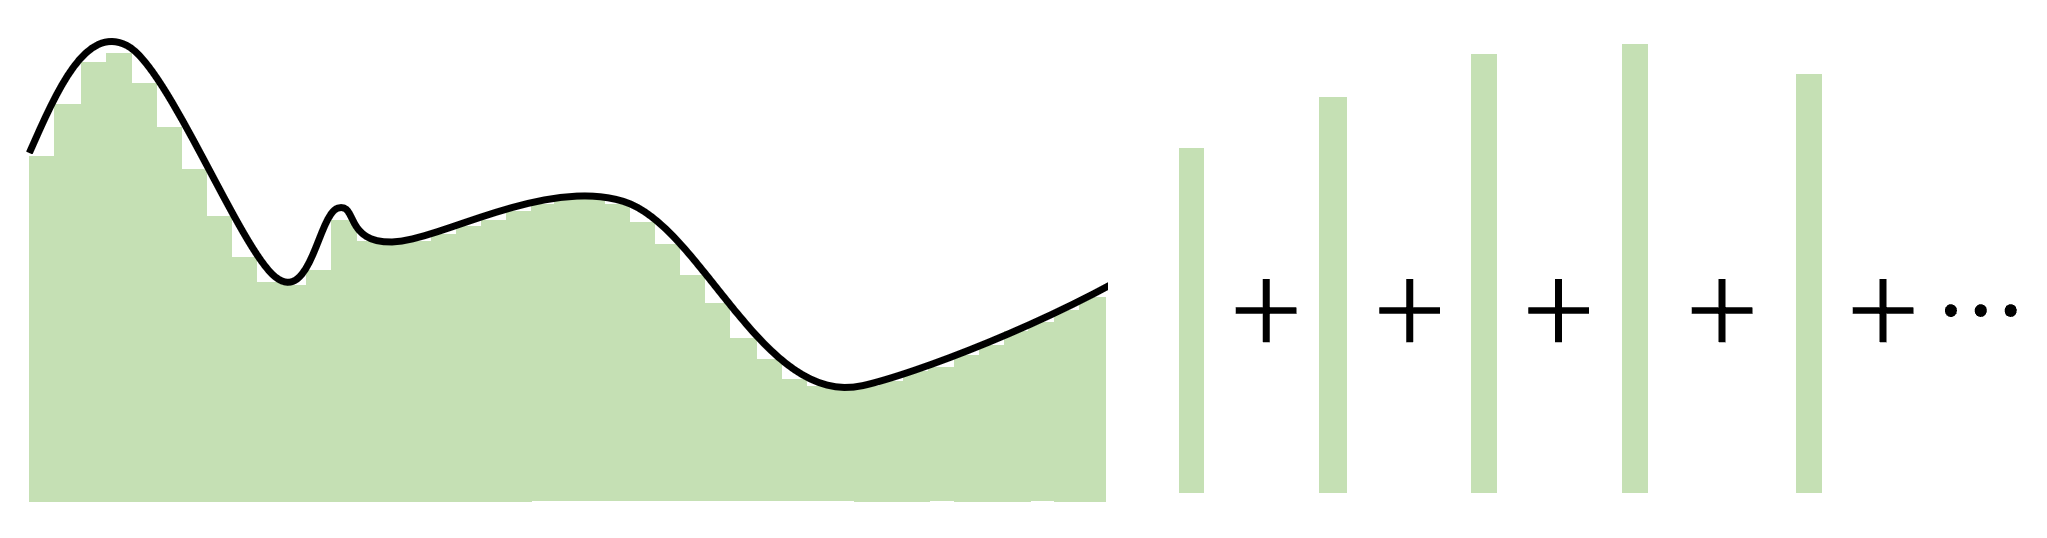
\includegraphics[scale=0.2]{images/steps.png}
\end{center}

Высоту ступеньки определяют по-разному. Чаще всего как значение функции в середине выбранного отрезка $b_i = f(\frac{a_i + a_{i+1}}{2})$. Тогда всю функцию целиком можно приблизить суммой

$$
f(x) \approx \sum_{i=1}^n f \left( \frac{a_i + a_{i+1}}{2} \right) \cdot [a_i \ge x < a_{i+1}].
$$

Давайте попробуем описать с помощью нейрона одну из ступенек. Пуст высота этой ступеньки равна $b_i$. Шагать по оси $x$ мы будем с фиксированным шагом $h$, поэтому $a_{i+1} = a_i + h$.

\begin{center}
\begin{tikzpicture}
\draw [line width=1.pt] (0,0)--(1,0)--(1,3)--(0,3)--cycle;
\draw [->] (-0.3,0)--(-0.3,3);
\draw [->] (-0.3,3)--(-0.3,0);
\draw (-0.3, 1.5) node[left] {$b_i$};
\draw (0.2, -0.3) node[left] {$a_i$};
\draw (1, -0.3) node[right] {$a_i + h$};
\end{tikzpicture}
\end{center}

Если $x$, для которого мы ищем $f(x)$ попадает в полуинтервал, на котором задана наша ступенька, мы будем приближать $f(x)$ этой ступенькой. Ступенька состоит из двух линий. Выходит, что она будет описываться двумя нейронами. Если мы внутри ступеньки, значит $a_i \le x < a_i + h$. Пара нейронов должна сравнить $x$ с $a_i$ и $a_i + h$ и на основе этого принять решение. Можно записать попадание $x$ в ступеньку следующим образом:

$$
1 - [x < a_i] - [x \ge a_i + h]
$$

Если оба условия --- неправда, получаем $1$. Мы в ступеньке. Если хотя бы одно из них выполнено --- мы вылетаем за ступеньку. Оба сразу выполниться они не могут. Нарисуем это в виде нейрона. В качестве функции активации используем единичную ступеньку. 

\begin{center}
\begin{tikzpicture}
\draw [line width=1.pt] (-3, 1.5) circle (0.5cm) node {$x$};
\draw [line width=1.pt] (-3, -0.5) circle (0.5cm) node {$1$};
	
\draw [line width=1.pt] (-1,1)--(2,1)--(2,2)--(-1,2)--cycle;
\draw (-0.3, 1.5) node[right] {$[x < a_i]$};

\draw [line width=1.pt] (-1,-1)--(2,-1)--(2,0)--(-1,0)--cycle;
\draw (-0.8, -0.5) node[right] {$[x \ge a_i + h]$};

\draw [line width=1.pt] (-2.5,1.5) -- (-1,1.5);
\draw (-1.7, 2) node {$1$};
\draw [line width=1.pt] (-2.5,1.5) -- (-1,-0.5);
\draw (-2.1, 0.8) node[left] {$1$};
\draw [line width=1.pt] (-2.5,-0.5) -- (-1,1.5);
\draw (-1, -1) node[left] {$a_i + h$};
\draw [line width=1.pt] (-2.5,-0.5) -- (-1,-0.5);
\draw (-2.1, 0.2) node[left] {$a_i$};

\draw [line width=1.pt] (3,0)--(5,0)--(5,1)--(3,1)--cycle;
\draw [line width=1.pt] (3.3,0.2)--(4,0.2)--(4,0.8)--(4.7,0.8);
\draw [line width=1.pt] (2,1.5) -- (3,0.5);
\draw (3, 1.5) node[left] {$-1$};
\draw [line width=1.pt] (2,-0.5) -- (3,0.5);
\draw (3, -0.5) node[left] {$-1$};

\draw [line width=1.pt] (4, 2.5) circle (0.5cm) node {$1$};
\draw [line width=1.pt] (4,2) -- (4,1);
\draw (4, 1.5) node[right] {$1$};

\draw [->] (5,0.5) -- (6,0.5);
\draw (5.2, 0.8)  node[right] {$b_i$};
\end{tikzpicture}
\end{center}

Нарисуем такую сетку для каждой ступеньки. Если мы попали в ступеньку, сетка будет выплёвывать со второго слоя единичку. Там мы будем умножать её на $b_i$ и посылать на внешний слой. Мы всегда будем попадать только в одну из ступенек, значит только один из слоёв выдаст нам $1$. Все остальные выдадут $0$. На внешнем слое нам остаётся только просуммировать всё, что к нам пришло и выдать ответ. Чем больше ступенек мы добавляем в модель, тем точнее наша апроксимация. 
\end{sol} 

% \newpage 

%%%-------------------------------------------
\begin{problem}{(число параметров)}
Та, кому принадлежит машин лёрнинг собирается обучить полносвязную нейронную сеть для решения задачи регрессии, На вход в ней идёт $12$ переменных, в сетке есть $3$ скрытых слоя. В первом слое $300$ нейронов, во втором $200$, в третьем $100$.  Сколько параметров предстоит оценить Маше?
\end{problem}

\begin{sol} 
Нам нужно решить довольно простую комбинаторную задачку. Связи в нашей сетке проведены между всему нейронами. Не забываем учесть, что у каждого нейрона есть константа. Получается, что всего параметров будет

\[
(12 + 1) \cdot 300 + (300 + 1) \cdot 200 + (200 + 1) \cdot 100 + (100 + 1) \cdot 1.
\]

\end{sol} 


\newpage 

% !TEX root = main.tex

%%%-------------------------------------------
\section*{Листочек 2: что выплёвывает нейросеть} 
\addcontentsline{toc}{section}{Листочек 2: что выплёвывает нейросеть}

\epigraph{Плюют в душу обычно те, кому не удалось в неё влезть.}{\textit{Пацанский паблик категории Б}}

%%%-------------------------------------------
\begin{problem}{(про сигмоиду)}
Любую $s$-образную функцию называют сигмоидой. Наиболее сильно прославилась под таким названием функция $f(t) = \frac{e^t}{1 + e^t}.$ Слава о ней добралась до Маши и теперь она хочет немного поисследовать её свойства\footnote{Часть задач украдена отсюда: \url{https://github.com/bdemeshev/mlearn_pro}}. 

\begin{enumerate}
	\item Что происходит при $t \to +\infty$? А при $t \to -\infty$?
	\item Как связаны между собой $f(t)$ и  $f(-t)$?
	\item Как связаны между собой $f'(t)$ и  $f'(-t)$?
	\item Как связаны между собой $f(t)$ и $f'(t)$? 
	\item Найдите $f(0)$, $f'(0)$ и $\ln f(0)$.
	\item Найдите обратную функцию $f^{-1}(t)$
	\item Как связаны между собой $\frac{d\ln f(t)}{dt}$ и $f(-t)$?
	\item Постройте графики функций $f(t)$ и $f'(t)$.
	\item Говорят, что сигмоида --- это гладкий аналог единичной ступеньки. Попробуйте построить на компьютере графики $f(t), f(10\cdot t), f(100\cdot t), f(1000\cdot t)$. Как они себя ведут? 
	\end{enumerate}
\end{problem} 

% \newpage 

%%%-------------------------------------------
\begin{problem}{(про $\logloss$)}
	У Маши три наблюдения, первое наблюдение --- кит, остальные --- муравьи. Киты кодируются $y_i = 1$, муравьи --- $y_i = 0$.  В качестве регрессоров Маша берёт номера наблюдений $x_i = i$. После этого Маша оценивает логистическую регрессию с константой. В качестве функции потерь используются логистические потери. 
	
	\begin{enumerate}
		\item Выпишите для данной задачи функцию потерь, которую минимизирует Маша.
		\item При каких оценках коэффициентов логистической регрессии эта функция достигает своего минимума?
	\end{enumerate}
\end{problem}

%%%-------------------------------------------
\begin{problem}{(про $\softmax$)}
	Маша чуть внимательнее присмотрелась к своему третьему наблюдению и поняла, что это не кит, а бобёр. Теперь ей нужно решать задачу классификации на три класса. Она решил использовать для этого нейросеть с softmax-слоем на выходе. 
	
	Маша уже обучила нейронную сетку и хочет построить прогнозы для двух наблюдений. Слой, который находится перед $\softmax$ выдал для этих двух наблюдений следующий результат: $(1, -2, 0)$ и $(0.5, -1, 0)$.
	
	\begin{enumerate}
		\item Чему равны вероятности получить кита, муравья и бобра для этих двух наблюдений? 
		
		\item Пусть первым был кит, а вторым бобёр.  Чему будет равна $\logloss$-ошибка? 
		
		\item Пусть у Маши есть два класса. Она хочет выучить нейросеть. Она может учить нейронку с одним выходом и сигмоидой в качестве функции активации либо нейронку с двумя выходами и $\softmax$ в качестве функции активации. Как выходы этих двух нейронок взаимосвязаны между собой? 
		
		\item  Объясните, почему $\softmax$  считают сглаженным вариантом максимума.
	\end{enumerate}
\end{problem}

% \begin{sol} 
% В решении нарисовать изокванты
% http://www.johndcook.com/blog/2010/01/13/soft-maximum/

% Чтобы найти максимум мы обычно используем функцию $f(x,y) = \max(x,y)$. Давайте нарисуем линии уровня такой функции. Они будут острыми 

% \todo[inline]{Картинка}

% Теперь рассмотрим мягкий максимум $f(x, y) = e^x$


% % [1,−2,0]→[e1,e−2,e0]=[2.71,0.14,1]→[0.7,0.04,0.26]
% % [0.5,−1,0]→[e0.5,e−1,e0]=[1.65,0.37,1]→[0.55,0.12,0.33]


%\begin{frame}{Важный нюанс}
%\begin{wideitemize} 
%\item При поиске Softmax мы ищем экспоненты, в памяти компьютера может произойти переполнение из-за больших чисел
%
%\item  Если добавить ко всем входам нейронки одинаковую константу, значение Sofrmax не изменится: 
%
%\[ 
%\frac{e^{z_i + c}}{\sum_{k=1}^K e^{z_k + c}} = \frac{ e^c \cdot e^{z_i } }{e^c \cdot \sum_{k=1}^K e^{z_k} }   = 	\frac{e^{z_i}}{\sum_{k=1}^K e^{z_k }} 
%\] 
%
%\item  Обычно считают устойчивый к переполнению Softmax: 
%
%\[
%\Softmax(z_1, \ldots, z_{K}) = \Softmax(z_1 - \max_i (z_i), \ldots, z_{K} - \max_i (z_i))
%\]
%
%\end{wideitemize}
%\end{frame}

% \end{sol} 

%%%-------------------------------------------
\begin{problem}{(про разные выходы)}
Та, в чьих руках находится лёрнинг, решила немного поэкспериментировать с выходами из своей сетки. 

\begin{enumerate}
	\item  Для начала Маша решила, что хочет решать задачу классификации на два класса и получать на выходе вероятность принадлежности к первому. Что ей надо сделать с последним слоем сетки? 
	
	\item  Теперь Маша хочет решать задачу классификации на $K$ классов. Что ей делать с последним слоем? 
	
	\item  Новые вводные! Маша хочет спрогнозировать рейтинг фильма на "Кинопоиске". Он измеряется по шкале от $0$ до $10$ и принимает любое непрерывное значение. Как Маша может приспособить для этого свою нейронку? 
	
	\item У Маши есть куча новостей. Каждая новость может быть спортивной, политической или экономической. Иногда новость может относится сразу к нескольким категориям. Как Маше собрать нейросетку для решения этой задачи?  Как будет выглядеть при этом функция ошибки? 
	
	\item  У Маши есть картинки с уточками и чайками. Маша хочет научить нейросеть искать на картинке птицу, обводить её в прямоугольник (bounding box), а затем классифицировать то, что попало в прямоугольник. Как должен выглядеть выход из такой нейросети? Как должна выглядеть функция потерь? 
	
	\item  Маша задумалась, как можно спрогнозировать число людей в кафе так, чтобы на выходе сетка всегда прогнозировала целое число. Надо ли как-то при этом менять функцию потерь?  
	
	\textbf{Hint:} вспомните про пуассоновскую регрессию.
\end{enumerate}
\end{problem}





\newpage 

% !TEX root = main.tex

%%%-------------------------------------------
\section*{Листочек 3: пятьдесят оттенков градиентного спуска}
\addcontentsline{toc}{section}{Листочек 3: пятьдесят оттенков градиентного спуска}

\epigraph{Повторять до сходимости --- это как жарить до готовности}{\textit{Неизвестный студент Вышки}}

\begin{problem}{(50 оттенков спуска)}
	Маша Нестерова, хозяйка машин лёрнинга\footnote{Лёрнинг ей папа подарил},  собрала два наблюдения: $x_1 = 1, x_2 = 2$, $y_1 = 2, y_2 = 3$ и собирается обучить линейную регрессию $y = w \cdot x$.  Маша очень хрупкая девушка, и ей не помешает помощь. 

	\begin{enumerate}
		\item Получите теоретическую оценку методом наименьших квадратов.
		
		\item  Сделайте три шага градиентного спуска. В качестве стартовой точки используйте $w_0 = 0$.  В качестве скорости обучения возьмите $\eta = 0.1$. 
		
		\item Сделайте четыре шага стохастического градиентного спуска.  Пусть в SGD сначала попадает первое наблюдение, затем второе. 
		
		\item Если вы добрались до этого пункта, вы поняли градиентный спуск. Маша довольна. Начинаем заниматься тупой технической бессмыслицей. Сделайте два шага Momentum SGD. Возьмите $\alpha = 0.9, \eta = 0.1$
		
		\item  Сделайте два шага Momentum SGD с коррекцией Нестерова. 
		
		\item Сделайте два шага RMSprop.  Возьмите $\alpha = 0.9, \eta = 0.1$
		
		\item  Сделайте два шага Adam. Возьмём  $\beta_1 = \beta_2 = 0.9, \eta = 0.1$		
	\end{enumerate}
\end{problem}

\begin{sol} 
    \begin{enumerate}
	\item  Найдём теоретическую оценку стандартным МНК. Минимизируем MSE: 
	
	\[
	MSE = \frac{1}{2} \cdot ((2 - w)^2 + (3 - 2 w)^2) \to \min_{w}
	\]
	
	Берём производную, решаем уравнение и получаем ответ: 
	\[
	- (2 - w)  - 2 (3 - 2 w) = 0 \Rightarrow \hat w = \frac{8}{5} = 1.6
	\]
	
	\item  Чтобы сделать три шага градиентного спуска, нужно найти градиент. Наша функция потерь выглядит как 
	
	\[
	L(w) = (y - w x)^2.
	\]
	
	Мы подбираем один параметр, значит градиентом в данном случае будет просто одно число --- производная по этому параметру. 
	
	\[ 
	 \nabla L(w_0, x, y) = \frac{\partial L}{\partial w} = -2 x (y - w x).
	\]
	
   Стартовая точка $w_0 = 0$. Мы хотим сделать шаг 
   
   \[
   w_1 = w_0 - \eta \cdot \nabla L(w_0)
   \]
	
	Посчитаем градиент в точке $w_0$ по всей выборке: 
	
	\[
	\nabla L(w_0) = \frac{1}{n} \cdot \sum_{i = 1}^n 	\nabla L(w_0, x_i, y_i)  = \frac{1}{2} \cdot (-2(2- w_0) - 2\cdot 2(3 - 2 w_0)) = -8
	\]
	
	Делаем \textbf{первый шаг:} 
	
	\[
	w_1 = 0 + 0.1 \cdot 8 = 0.8
	\]
	
   По аналогии, \textbf{второй шаг:}
	\begin{equation*}
	\begin{aligned}
	& \nabla L(w_1) =  \frac{1}{2} \cdot (-2(2 - w_1) - 2\cdot 2(3 - 2 w_1)) = -4 \\
	& w_2 = w_1 - \eta \cdot \nabla L(w_1) = 0.8 + 0.1 \cdot 4  = 1.2 
	\end{aligned}
	\end{equation*}
	
	По аналогии, \textbf{третий шаг:}
	\begin{equation*}
	\begin{aligned}
	& \nabla L(w_2) =  \frac{1}{2} \cdot (-2(2 - w_2) - 2\cdot 2(3 - 2 w_2)) = -2 \\
	& w_3 = w_2 - \eta \cdot \nabla L(w_2) = 1.2 + 0.1 \cdot 2  = 1.4
	\end{aligned}
	\end{equation*}
	
	\item Теперь то же самое, на градиентный спуск стохастический. Мы будем считать $\nabla(w_t)$ не как среднее по всей выборке, а как значение градиента в одной случайно выбранной точке. 
	
	\textbf{Первый шаг:} 
        \begin{equation*}
        \begin{aligned}
        & \nabla L(w_0) =  -2(2 - w_0 \cdot 1) = -4 \\
        & \beta_1 = w_0 - \eta \cdot \nabla L(w_0) = 0 + 0.1 \cdot 4  = 0.4
        \end{aligned}
        \end{equation*}
    	
    \textbf{Второй шаг:} 
        \begin{equation*}
        \begin{aligned}
        & \nabla L(w_1) =  -2 \cdot 2 \cdot (3 - w_1 \cdot 2) = - 8.8 \\
        & w_2 = w_1 - \eta \cdot \nabla L(w_1) = 0.4 + 0.1 \cdot 8.8  = 1.28
        \end{aligned}
        \end{equation*}	
	
    \textbf{Третий шаг:} 
        \begin{equation*}
        \begin{aligned}
        & \nabla L(w_2) =  -2(2 - w_1 \cdot 1) = -1.44 \\
        & w_3 = w_2 - \eta \cdot \nabla L(w_2) = 1.28 + 0.144 = 1.424
        \end{aligned}
        \end{equation*}	
    	
    \textbf{Четвёртый шаг:} 
        \begin{equation*}
        \begin{aligned}
        & \nabla L(w_3) =  -2 \cdot 2(3 - w_3 \cdot 2) \\
        & w_4 = w_3 - \eta \cdot \nabla L(w_4) = 1.424 + 0.1 \cdot 0.608  = 1.4848
        \end{aligned}
        \end{equation*}	

    \item Автор не очень хочет расписывать решение дальнейших четырёх пунктов. Но вы обязательно это сделайте. 
    \end{enumerate} 
\end{sol}


%%%%-------------------------------------------
\begin{problem}{(логистическая регрессия)}
Маша решила, что нет смысла останавливаться на обычной регрессии, когда она знает, что есть ещё и логистическая:

\begin{equation*}
\begin{aligned}
& z  = w \cdot x \qquad p = P(y = 1) = \frac{1}{1 + e^{-z}} \\
& \logloss = -[ y \cdot \ln p + (1 - y) \cdot \ln (1 - p) ]
\end{aligned}
\end{equation*}

Запишите формулу, по которой можно пересчитывать веса в ходе градиентного спуска для логистической регрессии. 

Оказалось, что $x = -5$, а $y = 1$. Сделайте один шаг градиентного спуска, если $w_0 = 1$, а скорость обучения $\gamma = 0.01$. 
\end{problem}

\begin{sol}
Сначала нам надо найти $\logloss'_{\beta}$. В принципе в этом и заключается вся сложность задачки. Давайте подставим вместо $\hat p $ в $\logloss$ сигмоиду. 

$$
\logloss = -1 \left (y \cdot \ln \left( \frac{1}{1 + e^{-z}} \right)  + (1 - y) \cdot \ln \left ( 1 - \frac{1}{1 + e^{-z}} \right ) \right)
$$
	
Теперь подставим вместо $z$ уравнение регрессии:
	

$$
\logloss = -1 \left (y \cdot \ln \left( \frac{1}{1 + e^{-w \cdot x}} \right)  + (1 - y) \cdot \ln \left ( 1 - \frac{1}{1 + e^{- w \cdot x}} \right ) \right)
$$

Это и есть наша функция потерь.  От неё нам нужно найти производную. Давайте подготовимся. 

\indef{Делай раз,} найдём производную $\logloss$ по $\hat p$: 
$$
\logloss'_{\hat p} = -1 \left(y \cdot \frac{1}{\hat p} - (1 - y) \cdot \frac{1}{(1 - p)} \right)
$$

\indef{Делай два,} найдём производную $\frac{1}{1 + e^{-w x}} $ по $w$: 
\begin{multline*}
\left(  \frac{1}{1 + e^{-w x}}   \right)'_{w}  = - \frac{1}{(1 + e^{-w x})^2} \cdot e^{-w x} \cdot (-x) =\frac{1}{1 + e^{-w x}}  \cdot \frac{e^{-w x}}{1 + e^{-w x}} \cdot x  = \\ = \frac{1}{1 + e^{-w x}}  \cdot  \left(1 - \frac{1}{1 + e^{-w x}}  \right) \cdot x
\end{multline*}

По-другому это можно записать как $\hat p \cdot (1 - \hat p) \cdot x$.  

\indef{Делай три,} находим полную производную:
\begin{multline*}
\logloss'_{\beta} = -1 \left(y \cdot \frac{1}{\hat p}  \cdot  \hat p \cdot  \left(1 - \hat p)  \right) \cdot x  - (1 - y) \cdot \frac{1}{(1 - \hat p)} \cdot  \hat p \cdot  \left(1 - \hat p)  \right) \cdot x \right) = \\ =  -y \cdot \left( 1 - \hat p \right) \cdot x + (1 - y) \cdot  \hat p  \cdot x =  (-y + y \hat p  + \hat p - y \hat p ) \cdot x = (\hat p - y) \cdot x
\end{multline*}
	
Найдём значение производной в точке $w_0 = 1$ для нашего наблюдения $x = -5, y=1$: 
$$
\left(\frac{1}{1 + e^{-1 \cdot (-5)}}  - 1 \right) \cdot (-5)  \approx  4.96
$$

Делаем шаг градиентного спуска: 
$$
w_1 = 1 - 0.01 \cdot 4.96 \approx 0.95
$$	
\end{sol} 

\begin{problem}{(вопросики)}
Убедитесь, что вы можете дать ответы на следующие вопросы: 

\begin{itemize} 
    \item  Как вы думаете, почему считается, что SGD лучше работает для оптимизации функций, имеющих больше одного экстремума?
    
    \item  Предположим, что у функции потерь есть несколько локальных минимумов. Как можно адаптировать градиентный спуск так, чтобы он находил глобальный минимум чаще?
    
    \item Что будет происходить со стохастическим градиентным спуском, если длина его шага не будет уменьшаться от итерации к итерации? 
\end{itemize} 
\end{problem} 


\begin{problem}{(скорости обучения)}
    В стохастическом градиентном спуске веса изменяются по формуле
    
    \[
    w_t = w_{t-1} - \eta_t \cdot \nabla L(w_{t-1}, x_i, y_i),
    \] где наблюдение $i$ выбрано случайно, скорость обучения зависит от номера итерации. 
    
    Условия Роббинса-Монро гарантируют сходимость алгоритма к оптимуму для выпуклых дифференцируемых функций. Они говорят, что ряд из скоростей $\sum_{t=0}^{\infty} \eta_t$ должен расходиться, а ряд $\sum_{t=0}^{\infty} \eta_t^2$ сходиться. То есть скорость спуска должна падать не слишком медленно, но и не слишком быстро. Какие из последовательностей, перечисленных ниже, можно использовать для описания изменения скорости алгоритма? 
    
    \begin{enumerate} 
        \item $\eta_t = \frac{1}{t}$ % да
        \item $\eta_t = \frac{0.1}{t^{0.3}}$
        \item $\eta_t = \frac{1}{\sqrt{t}}$
        \item $\eta_t = \frac{1}{t^2}$
        \item $\eta_t = e^{-t}$
        \item $\eta_t = \lambda \cdot \left(\frac{s_0}{s_0 + t} \right)^p,$ где $\lambda, p$ и $s_0$ --- параметры
    \end{enumerate} 
\end{problem} 





% \newpage 

% % !TEX root = main.tex

%%%-------------------------------------------
\section*{Листочек 4: матричное дифФфФфФференцирование}

\epigraph{ $\bigg(\text{ 
\includegraphics[scale=0.08]{tree1.png}} \bigg)^T = $  
\includegraphics[scale=0.08]{tree2.png} }{<<Джек и бобовый стебель>> (1890)}

% Эта часть виньетки необязательна для изучения. В ней мы подробно поговорим про матричные производные. С их помощью удобно заниматься оптимизацией, в том числе бэкпропом\footnote{Часть задач взята из \href{https://github.com/bdemeshev/mlearn\_pro/blob/master/mlearn\_pro.pdf}{прототипа задачника по ML  Бориса Демешева}, часть из \href{https://github.com/esokolov/ml-course-hse}{конспектов по ML Жени Соколова}}.


%%%-------------------------------------------
\begin{problem}{}	
	Найдите следующие производные:
	\begin{enumerate}	
	
	    \item $f(x) = x^2$, где $x$ скаляр
		
		\item $f(x) = a^T x$, где  $a$  и $x$ векторы размера $1 \times n$ 
		
		\item $f(x) = x^T A x$, где $x$ вектор размера $1 \times n$, $A$ матрица размера $n \times n$
		
 		\item $f(x) = \ln(x^T A x)$, где $x$ вектор размера $1 \times n$, $A$ матрица размера $n \times n$
		
		\item $f(x) = a^TXAXa$, где $x$ вектор размера $1 \times n$, $A$ матрица размера $n \times n$
		
 		\item $f(x) = x x^T x$,  где $x$ вектор размера $1 \times n$
	\end{enumerate}
\end{problem} 
\begin{sol}


Зачем нам нужно научиться искать матричные производные? \indef{Машинное обучение --- это сплошная оптимизация.} В нём мы постоянно вынуждены искать минимум какой-нибудь штрафной функции. Матричные производные довольно сильно в этом помогают\footnote{В тексте про матричные производные я опирался на \href{http://www.machinelearning.ru/wiki/images/5/50/MOMO17_Seminar2.pdf}{этот конспект.} Для того, чтобы познакомиться с темой более широко, имеет смысл прочитать его.}. 

Когда мы работаем с одномерными функциями, для поиска любых производных нам хватает небольшой таблицы со стандартными случаями и пары правил. Для случая матриц все эти правила можно обобщить, а таблицы дополнить специфическими функциями вроде определителя. \indef{Удобнее всего оказывается работать в терминах «дифференциала» --- с ним можно не задумываться о промежуточных размерностях, а просто применять стандартные правила.}

Мы будем работать в этом конспекте со скалярами, векторами и матрицами. Нас будет интересовать, что именно мы дифференцируем, по чему мы дифференцируем и что получается в итоге.  

Строчными буквами мы будем обозначать векторы-столбцы и константы. Заглавными буквами мы будем обозначать матрицы. Производная столбца --- это столбец. Производная по столбцу --- это столбец. 

\[
x = \begin{pmatrix}x_1 \\ \ldots \\ x_n \end{pmatrix} \qquad X = \begin{pmatrix}x_{11} & \ldots & x_{1n} \\ \vdots & \ddots & \vdots \\ x_{n1} & \ldots & x_{nn}  \end{pmatrix}.
\]

Мы рассмотрим постепенно много разных входов и выходов,  и получим таблицу из канонических случаев. По строчкам будем откладывать то, откуда бьёт функция, то есть входы. По столбцам будем откладывать то, куда бьёт функция, то есть выходы. Для ситуаций обозначенных прочерками обобщения получить не выйдет. 

\begin{center} 
    \begin{tabular}{|c|c|c|c|}
    \hline
        & скаляр & вектор & матрица \\
    \hline 
    скаляр & $f'(x) \dx{x}$  &  $\mathfrak{J} * \dx{x}$  & ---          \\
    \hline
    вектор & $\nabla f^T \dx{x}$    &   $\mathfrak{J} \dx{x}$     &  ---        \\
    \hline
    матрица & $\tr(\nabla f^T \dx{X})$    &    ---    & ---        \\
    \hline
    \end{tabular}
\end{center} 

Символом $\nabla^T f$ обозначается градиент (вектор из производных). Символом $\mathfrak{J}$ обозначена матрица Якоби. Символом $H$ мы будем обозначать матрицу Гессе из вторых производных. 

\begin{enumerate} 
\item Начнём с уже известного нам случая: функция бьёт из скаляров в скаляры

\[
f(x) : \RR \to \RR.
\]

Примером такой функции может быть $f(x) = x^2$. Мы знаем, что по таблице производных $f'(x) = 2x$. Также мы знаем, что \indef{дифференциал} --- это линейная часть приращения функции, а \indef{производная} --- это предел отношения приращения функции к приращению аргумента при приращении аргумента стремящемся к нулю.

Грубо говоря,  дифференциал помогает представить приращение функции в линейном виде

\[
\dx{f(x)} = f'(x) \dx{x}.
\]

Если мы находимся в какой-то точке $x_0$ и делаем из неё небольшое приращение $\dx{x},$ то наша функция изменится примерно на $\dx{f(x)}$. \indef{Оказывается, что именно в терминах дифференциалов удобно работать с матричными производными.}

Свойства матричных дифференциалов очень похожи на свойства обычных. Надо только не забыть, что мы работаем с матрицами.

\begin{equation*}
    \begin{aligned} 
    & \dx{(XY)} = \dx{X}Y + X\dx{Y}, \quad \dx{X}Y \ne Y\dx{X} \\
    & \dx{(\alpha X + \beta Y)} = \alpha \dx{X} + \beta \dx{Y} \\
    & \dx{(X^T)} = (\dx{X})^T \\
    & \dx{A} = 0, \quad A - \text{матрица из констант}
    \end{aligned} 
\end{equation*}

Чтобы доказать все эти свойства достаточно просто аккуратно расписать их. Кроме этих правил нам понадобится пара трюков по работе со скалярами. Если $s$ --- скаляр размера $1 \times 1$, тогда $s^T = s$ и $\tr(s) = s$, где $\tr$ --- операция взятия следа матрицы. 

С помощью этих преобразований мы будем приводить дифференциалы к каноническому виду и вытаскивать из них производные. 

\item Рассмотрим вторую ситуацию из таблицы, функция бьёт из векторов в скаляры. Это обычная функция от нескольких аргументов

\[
f(x) : \RR^n \to \RR.
\]

Такие производные мы брать также умеем. Если мы хотим найти производную функции $f(x_1, x_2, \ldots, x_n)$, нам надо взять производную по каждому аргументу и записать их все в виде вектора. Такой вектор \indef{называют градиентом} 

\[
\nabla f = \begin{pmatrix} \frac{\partial f}{\partial x_1} \\ \frac{\partial f}{\partial x_2} \\ \ldots  \\ \frac{\partial f}{\partial x_n} \end{pmatrix}
\]

Если умножить градиент на вектор приращений, у нас получится дифференциал

\[
\dx{f(x)} = \nabla f^T \dx{x} = \begin{pmatrix} \frac{\partial f}{\partial x_1} & \frac{\partial f}{\partial x_2} & \ldots  & \frac{\partial f}{\partial x_n} \end{pmatrix} \begin{pmatrix} \dx{x_1} \\ \dx{x_2} \\ \ldots  \\ \dx{x_n} \end{pmatrix} = \frac{\partial f}{\partial x_1} \cdot \dx{x_1} + \frac{\partial f}{\partial x_2} \cdot \dx{x_2} + \ldots +\frac{\partial f}{\partial x_n} \cdot \dx{x_n}.
\]

При маленьком изменении $x_i$ на $\dx{x_i}$ функция будет при прочих равных меняться пропорционально соответствующей частной производной. Посмотрим на конкретный пример, \indef{скалярное произведение}. Можно расписать умножение одного вектора на другой в виде привычной нам формулы

\begin{equation*}
\underset{[1 \times 1]}{f(x)} = \underset{[1 \times n]}{a^T} \cdot \underset{[n \times 1]}{x} = \begin{pmatrix} a_1 & a_2 & \ldots &a_n \end{pmatrix} \cdot \begin{pmatrix} x_1 \\ x_2 \\ \ldots  \\ x_n \end{pmatrix} = a_1 \cdot x_1 + a_2 \cdot x_2 + \ldots + a_n \cdot x_n.
\end{equation*} 

Из неё чётко видно, что $\frac{\partial f}{\partial x_i} = a_i$. Увидев это мы можем выписать градиент функции 

\[
\nabla f = \begin{pmatrix} \frac{\partial f}{\partial x_1} \\ \frac{\partial f}{\partial x_2} \\ \ldots  \\ \frac{\partial f}{\partial x_n} \end{pmatrix} = \begin{pmatrix} a_1 \\ a_2 \\ \ldots  \\ a_n \end{pmatrix} = a,
\]

теперь можно записать дифференциал

\[
\dx{f} = a^T \dx{x} = \frac{\partial f}{\partial x_1} \cdot \dx{x_1} + \frac{\partial f}{\partial x_2} \cdot \dx{x_2} + \ldots +\frac{\partial f}{\partial x_n} \cdot \dx{x_n} = a_1 \cdot \dx{x_1} + a_2 \cdot \dx{x_2} + \ldots + a_n \cdot \dx{x_n}.
\]

В то же самое время можно было бы просто воспользоваться правилами нахождения матричных дифференциалов

\[
\dx{f} =  \dx{a^T x} = a^T \dx{x} = \nabla f^T \dx{x},
\]

откуда $ \nabla f = a$. Производная найдена. При таком подходе нам не надо анализировать каждую частную производную по отдельности. Мы находим одним умелым движением руки сразу же все производные. Давайте немного усложним задачу и увидим его мощь во всей красе.

\item Функция по-прежнему бьёт из векторов в скаляры. Попробуем перемножить все матрицы и расписать её в явном виде по аналогии со скалярным произведением 


\begin{equation*}
\underset{[1 \times 1]}{f(x)} = \underset{[1 \times n]}{x^T} \cdot \underset{[n \times n]}{A} \cdot \underset{[n \times 1]}{x} = \sum_{i = 1}^n \sum_{j=1}^n a_{ij} \cdot x_i \cdot x_j.
\end{equation*} 

Если продолжить в том же духе, мы сможем найти все частные производные, а потом назад вернём их в матрицу. Единственное, что смущает --- \indef{мы делаем что-то неестественное.} Всё было записано в красивом компактном матричном виде, а мы это испортили. А что, если множителей будет больше? Тогда суммы станут совсем громоздкими, и мы легко запутаемся. 

При этом, если воспользоваться тут правилами работы с матричными дифференциалами, мы легко получим красивый результат

\[
\dx{f} =  \dx{x^T A x} =  \dx{(x^T)} A x + x^T \dx{(Ax)} =  \dx{(x^T)} A x + x^T \underset{\dx{A} = 0}{\dx{(A)}} x + x^T A \dx{(x)}.
\]

Заметим, что $\dx{(x^T)} A x$ это скаляр. Мы перемножаем матрицы с размерностями $1 \times n$, $n \times n$ и $n \times 1$. В результате получается размерность $1 \times 1$. Мы можем смело транспонировать скаляр, когда нам это надо. Эта операция никак не повлияет на результат

\[
\dx{f} = \dx{(x^T)} A x + x^T A \dx{(x)} = x^T A^T \dx{x}  + x^T A \dx{x} = x^T(A^T + A) \dx{x}.
\]

Мы нашли матричный дифференциал и свели его к каноничной форме 

\[
\dx{f} = \nabla^T f \dx{x} = x^T(A^T + A) \dx{x}
\]

Получается, что искомая производная $\nabla f = (A + A^T) x$. Обратите внимание, что размерности не нарушены и мы получили столбец из производных, то есть искомый градиент нашей функции $f$. 

По аналогии мы легко можем найти вторую производную. Для этого надо взять производную производной. Функция $g(x) = (A + A^T) x$ бьёт из векторов в вектора

\[
f(X) : \RR^n \to \RR^m.
\]

На самом деле с такой ситуацией мы также знакомились на математическом анализе. Если $n=1$ то у нас есть $m$ функций, каждая из которых применяется к $x$. На выходе получается вектор 

\[
\begin{pmatrix} f_1(x) \\ f_2(x) \\ \ldots  \\ f_m(x). \end{pmatrix}
\]

Если мы хотим найти производную, нужно взять частную производную каждой функции по $x$ и записать в виде вектора. Дифференциал также будет представлять из себя вектор, так как при приращении аргумента на какую-то величину изменяется каждая из функций 

\[
\dx{f(x)} = \begin{pmatrix} \frac{\partial f_1}{\partial x} \\ \frac{\partial f_2}{\partial x} \\ \ldots  \\ \frac{\partial f_m}{\partial x} \end{pmatrix} * \begin{pmatrix} \dx{x} \\ \dx{x} \\ \ldots  \\ \dx{x} \end{pmatrix}  = \begin{pmatrix} \frac{\partial f_1}{\partial x} \dx{x} \\ \frac{\partial f_2}{\partial x} \dx{x} \\ \ldots  \\ \frac{\partial f_m}{\partial x} \dx{x} \end{pmatrix}.
\]

Под символом $*$ имеется в виду поэлементное умножение. Если $n > 1$, то аргументов на вход в такой вектор из функций идёт несколько, на выходе получается матрица 

\[
\begin{pmatrix} f_1(x_1) & f_1(x_2) & \ldots & f_1(x_n) \\ f_2(x_1)  & f_2(x_2) & \ldots & f_2(x_n)  \\ \ldots & \ldots & \ddots & \ldots  \\ f_m(x_1)  & f_m(x_2) & \ldots & f_m(x_n) \end{pmatrix}
\]

Производной такой многомерной функции будет матрица из частных производных каждой функции по каждому аргументу

\[
\begin{pmatrix} \frac{\partial f_1}{\partial x_1} & \frac{\partial f_1}{\partial x_2} & \ldots & \frac{\partial f_1}{\partial x_n} \\ \frac{\partial f_2}{\partial x_1}  & \frac{\partial f_2}{\partial x_2} & \ldots & \frac{\partial f_2}{\partial x_n}  \\ \ldots & \ldots & \ddots & \ldots  \\ \frac{\partial f_m}{\partial x_1}  & \frac{\partial f_m}{\partial x_2} & \ldots & \frac{\partial f_m}{\partial x_n} \end{pmatrix}.
\]

Дифференциал снова будет представлять из себя вектор

\[
\dx{f(x)} =  \begin{pmatrix} \frac{\partial f_1}{\partial x_1} & \frac{\partial f_1}{\partial x_2} & \ldots & \frac{\partial f_1}{\partial x_n} \\ \frac{\partial f_2}{\partial x_1}  & \frac{\partial f_2}{\partial x_2} & \ldots & \frac{\partial f_2}{\partial x_n}  \\ \ldots & \ldots & \ddots & \ldots  \\ \frac{\partial f_m}{\partial x_1}  & \frac{\partial f_m}{\partial x_2} & \ldots & \frac{\partial f_m}{\partial x_n} \end{pmatrix} \cdot  \begin{pmatrix} \dx{x_1} \\ \dx{x_2} \\ \ldots  \\ \dx{x_n} \end{pmatrix} =  \begin{pmatrix} \frac{\partial f_1}{\partial x_1} \dx{x_1} + \frac{\partial f_1}{\partial x_2} \dx{x_2} + \ldots + \frac{\partial f_1}{\partial x_n} \dx{x_n}  \\ \frac{\partial f_2}{\partial x_1} \dx{x_1} +  \frac{\partial f_2}{\partial x_2} \dx{x_2} + \ldots + \frac{\partial f_2}{\partial x_n} \dx{x_n}  \\ \ldots  \\ \frac{\partial f_m}{\partial x_1} \dx{x_1} + \frac{\partial f_m}{\partial x_2} \dx{x_2} + \ldots + \frac{\partial f_m}{\partial x_n} \dx{x_n} \end{pmatrix}.
\]

В обоих ситуациях мы можем записать дифференциал через матричное произведение. Вернёмся к поиску второй производной

\[
\dx{g(x)} = (A + A^T) \dx{x}.
\]

Выходит, что матрица из вторых производных для функции $f(x)$ выглядит как $A + A^T.$ Обратите внимание, что для этой ситуации в каноническом виде нет транспонирования. Когда мы вытаскиваем из записи дифференциала производную, нам не надо его применять.


\item Когда мы хотим найти производную  $f(x) = \ln(x^T A x)$, мы просто можем применить правила взятия производной от сложной функции $f(y) = \ln(y).$ К логарифму на вход идет скаляр, а значит его производная равна $\frac{1}{y}$. Выходит, что 

\[
\dx{f(x)} = \dx{\ln(y)} = \frac{1}{y} \dx{y} = \frac{1}{y} \dx{(x^T A x)} = \frac{1}{x^T A x} \cdot x^T(A^T + A) \dx{x}.
\]

В таких ситуация нужно быть осторожным и следить за тем, что на вход функции идёт скаляр. Если это не так, то ситуация усложняется и мы оказываемся в ситуации, где надо поднапрячься. Чуть ниже мы рассмотрим в качестве примера матричную экспоненту $\exp(X),$ где $X$ --- квадратная матрица. 


\item \label{tr_tr} Движемся к следующей ситуации. Функция бьёт из матриц в скаляры

\[
f(X) : \RR^{n \times k} \to \RR.
\]

В таком случае нам надо найти производную функции по каждому элементу матрицы, то есть дифференциал будет выглядеть как 

\[
\dx{f(X)} = f'_{x_{11}} \dx{x_{11}} + f'_{x_{12}} \dx{x_{12}} + \ldots + f'_{x_{nk}} \dx{x_{nk}}.
\]

Его можно записать в компактном виде через след матрицы как 
\[
\dx{f(X)} = \tr(\nabla f^T \dx{X}),
\] где 

\[
\nabla f = \begin{pmatrix} f'_{x_{11}} & \ldots & f'_{x_{1k}} \\ 
\hdots & \ddots & \hdots \\ 
f'_{x_{n1}} & \ldots & f'_{x_{nk}}
\end{pmatrix}
\]

Вполне естественен вопрос \indef{а почему это можно записать именно так?} Давайте попробуем увидеть этот факт на каком-нибудь простом примере. Пусть у нас есть две матрицы 

\[
A_{[2 \times 3]} = \begin{pmatrix} a_{11} & a_{12} & a_{13} \\ a_{21} & a_{22} & a_{23} \end{pmatrix} \qquad X_{[2 \times 3]} = \begin{pmatrix} x_{11} & x_{12} & x_{13} \\ x_{21} & x_{22} & x_{23} \end{pmatrix}.
\]

Посмотрим на то, как выглядит $\tr(A^T \dx{X})$. Как это не странно, он совпадает с дифференциалом 

\[\tr(A^T \dx{X}) = \tr \left( \begin{pmatrix} a_{11} & a_{21} \\ a_{12} & a_{22} \\ a_{13} &  a_{23} \end{pmatrix} \begin{pmatrix} \dx x_{11} & \dx x_{12} & \dx x_{13} \\ \dx x_{21} & \dx x_{22} & \dx x_{23} \end{pmatrix} \right),
\]

при произведении на выходе получаем матрицу размера $3 \times 3$

\[
\begin{pmatrix} a_{11} \dx x_{11} +  a_{21} \dx x_{21} & a_{11} \dx x_{12} +  a_{21} \dx x_{22} & a_{11} \dx x_{13} +  a_{21} \dx x_{23} \\ a_{12} \dx x_{11} +  a_{22} \dx x_{21} & a_{12} \dx x_{12} +  a_{22} \dx x_{22} & a_{12} \dx x_{13} +  a_{22} \dx x_{23} \\ a_{13} \dx x_{11} +  a_{23} \dx x_{21} & a_{13} \dx x_{12} +  a_{23} \dx x_{22} & a_{13} \dx x_{13} +  a_{23} \dx x_{23} \end{pmatrix}.
\]

\index{Когда мы берём её след, остаётся сумма элементов по диагонали. Это и есть требуемый дифференциал.} Дальше мы периодически будем пользоваться таким приёмом. Например,  величину 

\[ 
||X-A||^2 = \sum_{i,j} (x_{ij} - a_{ij})^2
\]

можно записать в матричном виде как 

\[
\tr((X-A)^T (X-A)).
\]



Итак, найдём производную от $f(X) = a^TXAXa$. Нам нужно выписать дифференциал и привести его к каноническому виду

Обратим внимание на то, что мы бьём из матриц в скаляры. Дифференциал будет по своей размерности совпадать со скаляром. Производная будет размера матрицы

\[
\dx{f(X)} = \dx{(a^TXAXa)} = \underset{[1 \times 1]}{a^T\dx{(X)}AXa} + \underset{[1 \times 1]}{a^TXA\dx{(X)}a}.
\]

Оба слагаемых, которые мы получаем после перехода к дифференциалу --- скаляры. Мы хотим представить дифференциал в виде $\tr(\text{нечто} \dx{X})$. След от скаляра это снова скаляр. Получается, что мы бесплатно можем навесить над правой частью наешго равенство знак следа и воспользоваться его свойствами

\begin{multline*}
\dx{f(X)} = \dx{(a^TXAXa)} = \tr(a^T\dx{(X)}AXa) + \tr(a^TXA\dx{(X)}a) = \\ = \tr(AXaa^T\dx{(X)}) + \tr(aa^TXA\dx{(X)}) = \\ = \tr(AXaa^T\dx{(X)} + aa^TXA\dx{(X)}) = \tr((AXaa^T + aa^TXA)\dx{(X)}).
\end{multline*}

Производная найдена, оказалось что это 

\[
\nabla f = (AXaa^T + aa^TXA)^T = aa^TX^TA^T + A^TXaa^T.
\]

Как бы мы нашли это, всё по-честному перемножив, даже боюсь себе представлять. 

\item Ещё один пример на ситуацию, когда функция бьёт из векторов в вектора

\[ 
\underset{[n \times 1]}{f(x)} = \underset{[n \times 1]}{x} \underset{[1 \times n]}{x^T}  \underset{[n \times 1]}{x}.
\]
В нём надо аккуратно вести себя со сложением матриц со скалярами. Берём дифференциал 

\[
\dx{f(x)} = \dx{xx^Tx} = \dx{x}x^Tx + x \dx{x^T} x + xx^T\dx{x}.
\]

В первом слагаемом пользуемся тем, что $x^Tx$ скаляр и его можно вынести перед дифференциалом. Этот скаляр умножается на каждый элемент вектора. Дальше мы захотим вынести дифференциал за скобку, чтобы не испортить матричное сложение, подчеркнём факт этого перемножения на каждый элемент единичной матрицей. Во втором слагаемом пользуемся тем, что $\dx{x^T} x$ скаляр и транспонируем его 
\[
\dx{f(x)} = \underset{[1 \times 1]}{x^Tx} \underset{[n \times n]}{I_n} \underset{[n \times 1]}{\dx{x}} + x x^T \dx{x} + xx^T\dx{x} = (x^Tx I_n + 2 x x^T)\dx{x}.
\]

Обратите внимание, что без единичной матрицы размерности у сложения поломаются. Получается, что наша производная выглядит как 

\[
\mathfrak{J} = x^Tx I_n + 2 x x^T = \begin{pmatrix} \sum x_i^2 + 2 x_1^2 & 2 x_1 x_2 & \ldots & 2 x_1 x_n \\
2 x_1 x_2 & \sum x_i^2 + 2 x_2^2 & \ldots & 2 x_2 x_n \\
\ldots & \ldots & \ddots &\ldots \\
2 x_1 x_n & 2 x_n x_2 & \ldots & \sum x_i^2 + 2 x_n^2 \\
\end{pmatrix}.
\]

Как и ожидалось, на выходе получилась матрица.


\item \indef{В нашей таблице. осталось ещё несколько ситуаций, которые остались вне поля нашего зрения.} Давайте их обсудим более подробно. Например, давайте посмотрим на ситуацию когда отображение бьёт из матриц в вектора

\[
f(X) : \RR^{n \times k} \to \RR^m.
\]

Тогда $X$ матрица, а $f(X)$ вектор. Нам надо найти производную каждого элемента из вектора $f(X)$ по каждому элементу из матрицы $X$. Получается, что $\frac{\partial f}{\partial X}$ --- это трёхмерная структура. Обычно в таких ситуациях ограничиваются записью частных производных либо прибегают к более сложным, многомерным методикам. Мы такие ситуации опустим. 
\end{enumerate} 
\end{sol}

\begin{problem}{}
Давайте пополним таблицу дифференциалов несколькими новыми функциями, специфичными для матриц. Найдём матричные дифференциалы функций: 
\begin{enumerate}
		\item $f(X) = X^{-1}$, где матрица $X$ размера $n \times n$
		
		\item  $f(X) = \det X$, где матрица $X$ размера $n \times n$
		
		\item $f(X) = \tr(X)$, где матрица $X$ размера $n \times n$
		
		\item Ещё больше матричных производных можно найти в книге The Matrix Cookbook\footnote{\url{https://www.math.uwaterloo.ca/~hwolkowi/matrixcookbook.pdf}}
	\end{enumerate}
\end{problem} 

\begin{sol} 
\begin{enumerate}
    \item Найдём производную обратной матрицы.  Тут логично вспомнить, что производная константы это ноль, обратная матрица определяется как $X^{-1} \cdot X = I_n$, а единичная матрица $I_n$ это как раз константа. Берём дифференциал с обеих сторон нашего равенства 
    
    \[
    \dx{X^{-1}} X + X^{-1} \dx{X} = \dx{I_n} = 0,
    \]
    
    отсюда получаем что 
    
    \[
    \dx{X^{-1}} = - X^{-1} \dx{X} X^{-1}.
    \]
    
    \item Определитель --- это функция, которая бьёт из матриц в скаляры. Его можно искать по-разному, один из способов --- разложение по строке
    
    \[
    \det X = \sum_{j = 1}^n x_{ij} (-1)^{i + j} M_{ij}, 
    \]
    
    где $M_{ij}$ --- дополнительный минор матрицы $X$. Берём дифференциал 
    
    \[
    \dx{(\det X)} = (-1)^{1 + 1} M_{11} \dx{x_{11}} + (-1)^{1 + 2} M_{12}  \dx{x_{12}} + \ldots  = \sum_{ij} A_{ji} \dx{x_{ij}} = \tr(A \dx{X}),
    \]
    
    где $A_{ij} = (-1)^{i +j} M_{ij},$ то есть $A$ --- матрица алгебраических дополнений. Трюк со следом аналогичен пункту \ref{tr_tr} из предыдущей задачи. Вспомним, что обратную матрицу можно получить отталкиваясь от алгебраических дополнений по формуле 
    
    \[
    X^{-1} = \frac{A}{\det X}.
    \]
    
    Выразим матрицу $A$ и подставим её а получившееся выше уравнение 
    
    \[
    \dx{(\det X)} = \tr(\det (X) X^{-1} \dx{X}),
    \]
    
    выходит что искомая производная равна 
    
    \[
    \nabla f = (\det X \cdot X^{-1})^T = \det X \cdot X^{-T}.
    \]
    
    \item По аналогии с определителем след бьёт из пространства матриц в пространство скаляров, получается 
    
    \[
    \dx{(\tr X)} = \tr(I_n \dx X).
    \]
    
    Это логично, так как след представляет из себя сумму диагональных элементов.
\end{enumerate} 
\end{sol}


%%%-------------------------------------------
\begin{problem}{}
	Рассмотрим задачу линейной регресии
	\[
	L(w) = (y - Xw)^T(y - Xw) \to \min_{w}.
	\]
	
	\begin{enumerate}
		\item Найдите $L(w)$, выведите формулу для оптимального $w$.
		\item Как выглядит шаг градиентного спуска в матричном виде?
		\item Найдите $\dx^2L(w)$. Убедитесь, что мы действительно в точке минимума. 
	\end{enumerate}
\end{problem}
\begin{sol} 
Ради интереса убедимся, что перед нами в качестве функции потерь используется именно MSE, в качестве $x_i$ будем обозначать $i-$ую строчку матрицы $X$

\[
(y - Xw)^T(y - Xw) = \begin{pmatrix} y_1 - x_1^Tw &  \ldots & y_n - x_n^Tw \end{pmatrix} \begin{pmatrix} y_1 - x_1^Tw \\  \ldots \\ y_n - x_n^Tw \end{pmatrix}   = \sum_{i=1}^n (y_i - x_i^Tw)^2.
\]

Найдём дифференциал для нашей функции потерь, держим в голове что производная берётся по вектору $w$ 

\begin{multline*}
\dx L = \dx[(y - Xw)^T(y - Xw)] = \dx[(y - Xw)^T] (y - Xw) + (y - Xw)^T\dx[(y - Xw)] = \\ = \dx[(-Xw)^T] (y - Xw) - (y - Xw)^TX\dx w = \\ = - \dx w^T X^T (y - Xw) - (y - Xw)^TX\dx w = -2 (y - Xw)^TX \dx w.
\end{multline*} 

Тут мы воспользовались тем, что $ \dx w^T X^T (y - Xw)$ это скаляр и его можно транспонировать. Производная найдена. Шаг градиентного спуска будет выглядеть как 

\[
w_t = w_{t-1} + \gamma \cdot 2X^T(y-Xw).
\]

Здесь $\gamma$ --- это скорость обучения. Приравняем производную к нулю, чтобы найти минимум для $w$. Получается система уравнений

\[
2X^T(y-Xw) = 0 \qquad  X^Ty = X^TX w \qquad w = (X^TX)^{-1} X^Ty.
\]

При решении системы мы сделали предположение, что матрица $X^TX$ обратима. Это так, если в матрице $X$ нет линейно зависимых столбцов, а также наблюдений больше чем переменных. Найдём вторую производную 

\[
\dx[-2X^T(y-Xw)] = 2X^TX \dx w.
\]

Выходит, что $H = 2X^TX$. Так как матрица $X^TX$ положительно определена, по критерию Сильвестра, мы находимся в точке минимума. 

Матрица $X^TX$ положительно определена по определению. Если для любого вектора $v \ne 0$ квадратичная форма $v^T X^TX v > 0$, матрица  $X^TX$ положительно определена. При перемножении $Xv$ у нас получается вектор. Обозначим его как $z$, значит $v^T X^TX v = z^T z = \sum_{i=1}^n z_i^2 > 0$. 

Выпишем в явном виде второй дифференциал 

\[
\dx^2 L = \dx w^T 2X^TX \dx w.
\]
\end{sol} 


%%%-------------------------------------------
\begin{problem}{}
	Найдите следующие производные:
	\begin{enumerate}
		\item $f(X) = \tr(AXB)$, где матрица $A$ размера $p \times m$, матрица $B$ размера $n \times p$, матрица $X$ размера $m \times n$.  % A^TB^T
		
		\item $f(X) = \tr(AX^TX)$, где матрица $A$ размера $n \times n$, матрица $X$ размера $m \times n$.  % XA + XA^T
		
		\item $f(X) = \ln \det X$ % X^{-1}
		
		\item $f(X) = \tr(AX^TXBX^{-T})$
		
		\item $f(X) = \det(X^TAX)$
		
		\item $f(x) = x^TAb$, где матрица $A$ размера $n \times n$, вектора $x$ и $b$ размера $n \times 1$. 
		
		\item $f(A) = x^TAb$. 
	\end{enumerate}
\end{problem}
\begin{sol} 
Проверить правильность своего решения можно в матричном калькуляторе\footnote{ \url{http://www.matrixcalculus.org/}}. Не забывайте, что $\tr(A) = \tr(A^T)$ и что под знаком следа можно циклически переставлять матрицы, если размерность не ломается. 
\end{sol} 


%%%-------------------------------------------
\begin{problem}{}
    В случае Ridge-регрессии минимизируется функция со штрафом:
	\[
	L(w) = (y - Xw)^T(y - Xw) + \lambda w^Tw,
	\]
	где $\lambda$ — положительный параметр, штрафующий функцию за слишком большие значения $w$.
	
	\begin{enumerate}
		\item Найдите $dL(w)$, выведите формулу для оптимального $w$.
		\item Как выглядит шаг градиентного спуска в матричном виде?
		\item Найдите $d^2L(w)$. Убедитесь, что мы действительно в точке минимума. 
	\end{enumerate}
\end{problem}
\begin{sol} 
\begin{equation*} 
\begin{aligned} 
& \dx L = 2 (y - Xw)^TX \dx w + 2\lambda w^T \dx{w} \\ 
& \nabla L(w) = 2 X^T (Xw - y) + 2\lambda w \\
& w = (X^TX + \lambda I)^{-1} X^Ty \\
& w_t = w_{t-1} - \gamma \cdot (2 X^T (Xw_{t-1} - y) + 2\lambda w_{t-1}) \\
& \dx^2 L = \dx{w^T}(2X^TX + 2\lambda)\dx{w} \\
& H = 2X^TX + 2\lambda \text{ положительно определена}
\end{aligned} 
\end{equation*} 

% Для Lasso-модели нужно рассмотреть два случая: 

% \begin{itemize} 
% \item $w \ge 0: \quad L(w) - (y - xw)^T(y-xw) + \lambda w$. Решив, получаем оптимальное значение 

% \[ w^{+} = \frac{x^Ty}{x^Tx} - \frac{\lambda}{2x^Tx}.\]

% \item $w < 0: \quad L(w) - (y - xw)^T(y-xw) - \lambda w$. Решив, получаем оптимальное значение 

% \[ w^{-} = \frac{x^Ty}{x^Tx} + \frac{\lambda}{2x^Tx}.\]
% \end{itemize} 

% Заметим, что $L(w)$ --- это парабола. Рассмотрим четыре ситуации положения $w^{+}$ и $w^{-}$ и получим ответ: 

% \begin{equation*} 
% \begin{aligned} 
% & w^{+} < 0, w^{-1} < 0 \Rightarrow \hat{w} = w^{-} \\
% & w^{+} > 0, w^{-1} > 0 \Rightarrow \hat{w} = w^{+} \\
% & w^{+} < 0, w^{-1} > 0 \Rightarrow \hat{w} = 0 \\
% & w^{+} > 0, w^{-1} < 0  \text{ этот случай невозможен.}
% \end{alligned} 
% \end{equation*} 
\end{sol}


%%%-------------------------------------------
\begin{problem}{}
	Пусть $x_i$ — вектор-столбец $k\times 1$, $y_i$ — скаляр, равный $+1$ или $-1$, $w$ — вектор-столбец размера $k\times 1$. Рассмотрим логистическую функцию потерь с $l_2$ регуляризацией
	\[
	L(w) = \sum_{i=1}^n \ln (1 + \exp(-y_ix_i^Tw)) + \lambda w^T w
	\]
	
	\begin{enumerate}
		\item Найдите $\dx L$;
		\item Найдите вектор-столбец $\nabla L$.
		\item Как для этой функции потерь выглядит шаг градиентного спуска в матричном виде? 
	\end{enumerate}
\end{problem}
\begin{sol} 
Используем весь арсенал, который обсудили выше. Начнём с одного слагаемого. Обозначим его как $y$. Это скаляр, значит

\[
\dx \ln y = \frac{1}{y} \dx y =  \frac{1}{\ln (1 + \exp(-y_ix_i^Tw))} \cdot -y_i \exp(-y_i x_i^T w) \cdot x_i^T \dx w.
\]

Выписываем дифференциал

\[
\dx L = \left( - \sum_{i=1}^n \frac{y_i \exp(-y_i x_i^T w)}{1 + \exp(-y_ix_i^Tw)} \cdot x_i^T + 2 \lambda w^T  \right) \dx{w}.
\]

Можно записать градиент с помощью сигмоиды $\sigma(z) = \frac{1}{1 + \exp(-z)}.$ Получится, что 

\[
\nabla L = \sum_{i=1}^n -y_i \sigma(-y_i x_i^T w) x_i + 2 \lambda w.
\]

Выходит, что шаг градиентного спуска можно записать как 

\[
w_t = w_{t-1} + \gamma \cdot \nabla L.
\]
\end{sol} 


%%%-------------------------------------------
\begin{problem}{}
	Упражняемся в матричном методе максимального правдоподобия.  Допустим, что выборка размера $n$ пришла к нам из многомерного нормального распределения с неизвестными вектором средних $\mu$ и ковариационной матрицей $\Sigma$. В этом задании нужно найти оценки максимального правдоподобия для $\hat \mu$ и $\hat \Sigma$.  Обратите внимание, что выборкой здесь будет не $x_1, \ldots, x_n$, а 
	\begin{equation*}
	\begin{pmatrix}
	x_{11}, \ldots, x_{n1} \\
	\ldots  \\ 
	x_{n1}, \ldots, x_{nm}
	\end{pmatrix}
	\end{equation*}
\end{problem}
\begin{sol} 

Плотность распределения для $m-$мерного вектора $y$ будет выглядеть как 
	
	\[ 
	f(x \mid \mu, \Sigma) = \frac{1}{(\sqrt{2 \pi})^m \cdot \sqrt{\det \Sigma}} \cdot \exp \left( - \frac{1}{2} \cdot (x - \mu)^T \Sigma^{-1} (x - \mu) \right).
	\]
	
	В силу того, что все наблюдения независимы, функция правдоподобия для выборки объёма $n$ примет вид: 
	
	\[
	L(x \mid \mu, \Sigma) = \frac{1}{(\sqrt{2 \pi})^{m \cdot n} \cdot \sqrt{\det \Sigma}^n} \cdot \exp \left( - \frac{1}{2} \cdot \sum_{i = 1}^n (x_i - \mu)^T \Sigma^{-1} (x_i - \mu) \right).
	\]
	
	Прологарифмировав правдоподобие, получим
	
	\[
	\ln L(x \mid \mu, \Sigma) = - \frac{m \cdot n}{2} \ln 2 \pi - \frac{n}{2} \ln \det \Sigma - \frac{1}{2} \sum_{i=1}^n (x_i - \mu)^T \Sigma^{-1} (x_i - \mu) 
	\]
	
	Нам нужно найти максимум этой функции по $\mu$  и $\Sigma$.  Начнём с $\mu$.  Аргумент $\Sigma$ будем считать константой. Обозначим такую функцию за $f(\mu)$. Эта функция бьёт с множества векторов в множество скаляров.  Значит дифференциал этой функции можно записать в виде: 
	
	\[ df(\mu) = \nabla f^T d \mu. \]
	
	Найдём этот дифференциал. Не будем забывать, что дифференциал от константы нулевой, а также что дифференциал суммы равен сумме дифференциалов
	
	\begin{multline*}
	d f(\mu) = -\frac{1}{2} \cdot d \sum_{i=1}^n (x_i - \mu)^T \Sigma^{-1} (x_i - \mu) = -\frac{1}{2} \cdot \sum_{i=1}^n d[(x_i - \mu)^T \Sigma^{-1} (x_i - \mu)] = \\ = -\frac{1}{2} \cdot \sum_{i=1}^n d[(x_i - \mu)^T] \Sigma^{-1} (x_i - \mu) + (x_i - \mu)^T \Sigma^{-1} d[(x_i - \mu)] = \\ =   \frac{1}{2} \cdot \sum_{i=1}^n d\mu^T \Sigma^{-1} (x_i - \mu) + (x_i - \mu)^T \Sigma^{-1} d\mu.
	\end{multline*}
	
	Первое слагаемое под суммой имеет размерность $1 \times m \cdot m \times m \cdot m \times 1$. Это константа. Если мы протранспонируем константу, ничего не изменится. Обратим внимание, что матрица $\Sigma$ симметричная и при транспонировании не меняется. Сделаем этот трюк 
	
	\begin{multline*}
	 \frac{1}{2} \cdot \sum_{i=1}^n d\mu^T \Sigma^{-1} (x_i - \mu) + (x_i - \mu)^T \Sigma^{-1} d\mu = \frac{1}{2} \cdot \sum_{i=1}^n  (x_i - \mu)^T \Sigma^{-1}  d\mu  + (x_i - \mu)^T \Sigma^{-1} d\mu = \\ = \frac{1}{2} \cdot \sum_{i=1}^n  [(x_i - \mu)^T \Sigma^{-1}  + (x_i - \mu)^T \Sigma^{-1} ] d\mu =  \left[  \cdot \sum_{i=1}^n  (x_i - \mu)^T \Sigma^{-1} \right] d\mu 
	\end{multline*}	
	
	Получается, что $f'(\mu) = \sum_{i=1}^n   \Sigma^{-1} (x_i - \mu)$.  Приравняв производную к нулю и домножив обе части уравнения слева на $\Sigma$, получим оптимальное значению $\mu$: 
	
	\begin{equation*}
	\begin{aligned}
	&\sum_{i=1}^n   \Sigma^{-1} (x_i - \hat \mu) = 0 \\
	&\sum_{i=1}^n   (x_i - \hat \mu) = 0 \\
	&\sum_{i=1}^n   x_i =  n \cdot \hat \mu \Rightarrow \hat \mu = \bar x.
	\end{aligned} 
	\end{equation*}
		
Не будем забывать, что в записях выше $x$ и $\mu$ были векторами-столбцами размерности $m \times 1$. В итоговом ответе они также являются векторами-столбцами такой размерности. 

Займёмся оценкой для $\Sigma.$ Аргумент $\mu$ будем считать константой. Обозначим такую функцию за $f(\Sigma)$

\[
f(\Sigma) = - \frac{n}{2} \ln \det \Sigma - \frac{1}{2} \sum_{i=1}^n (x_i - \mu)^T \Sigma^{-1} (x_i - \mu).
\]

Эта функция бьёт с множества матриц в множество скаляров. Значит дифференциал этой функции можно записать в виде: 

\[
d f(\Sigma) = \tr (\nabla f^T dx).
\]

Начнём с первого слагаемого. Для него нам понадобится вспомнить как выглядит дифференциал для определителя

\[
- \frac{n}{2} \frac{1}{\det \Sigma}  d[\det \Sigma]  = - \frac{n}{2} \frac{1}{\det \Sigma}  \tr( \det \Sigma \cdot \Sigma^{-T} d \Sigma) =   -  \tr( \frac{n}{2} \cdot \Sigma^{-1} d \Sigma).
\]

Теперь поработаем со вторым слагаемым. В нём нас интересует дифференциал обратной матрицы

\[
- \frac{1}{2} \sum_{i=1}^n (x_i - \mu)^T d[\Sigma^{-1}] (x_i - \mu) = \frac{1}{2} \sum_{i=1}^n (x_i - \mu)^T \Sigma^{-1} \cdot  d \Sigma \cdot \Sigma^{-1} (x_i - \mu). 
\]	
	
Под знаком суммы размерность каждого слагаемого $1 \times m \cdot m \times m \cdot m \times m \cdot m \times m \cdot m \times 1$. Это константа. Если мы возьмём от неё след, ничего не изменится. Взяв след, переставим внутри множители

\[
\frac{1}{2} \sum_{i=1}^n (x_i - \mu)^T \Sigma^{-1} \cdot  d \Sigma \cdot \Sigma^{-1} (x_i - \mu)  = \frac{1}{2} \sum_{i=1}^n \tr( \Sigma^{-1} (x_i - \mu) \cdot (x_i - \mu)^T \Sigma^{-1} \cdot  d \Sigma). 
\] 

Сумма следов --- след суммы. Объединяем наши слагаемые в месте. В первом множитель $n$ подменяем на сумму 

\[
d f(\Sigma) = \tr \left( \left [ - \frac{1}{2} \sum_{i = 1}^n \Sigma^{-1} + \Sigma^{-1} (x_i - \mu) \cdot (x_i - \mu)^T \Sigma^{-1} \right] d \Sigma \right)
\]

Забираем себе из-под знака дифференциала производную. Под знаком суммы после транспонирования ничего не поменяется. Приравниваем производную к нулю, домножим справа каждое слагаемое на $\Sigma$. На четвёртой строчке домножим слева на $\Sigma$: 

\begin{equation*}
\begin{aligned} 
 & \frac{1}{2} \sum_{i = 1}^n - \Sigma^{-1} + \Sigma^{-1} (x_i - \mu) \cdot (x_i - \mu)^T \Sigma^{-1}  = 0 \\
 & - n \cdot \Sigma^{-1} + \sum_{i = 1}^n  \Sigma^{-1} (x_i - \mu) \cdot (x_i - \mu)^T \Sigma^{-1}  = 0 \\
 & - n + \Sigma^{-1} \sum_{i = 1}^n  (x_i - \mu) \cdot (x_i - \mu)^T = 0 \\
 & - n \Sigma+ \sum_{i = 1}^n  (x_i - \mu) \cdot (x_i - \mu)^T = 0 \\
 &  \Sigma  = \frac{1}{n} \sum_{i = 1}^n  (x_i - \mu) \cdot (x_i - \mu)^T 
\end{aligned}
\end{equation*}
	
До оценок остался один шаг. Вспоминаем оценку для $\mu$, подставляем её в уравнение и получаем, что 

\[
\hat \Sigma = \frac{1}{n} \sum_{i = 1}^n  (x_i - \bar x) \cdot (x_i - \bar x)^T.
\]
	
Не забываем, что $x_i$ и $\bar x$ --- вектора размерности $m \times 1$. 
\end{sol} 


%%%-------------------------------------------
\begin{problem}{}
	Найдите симметричную матрицу $X$ наиболее близкую к матрице $A$ по норме Фробениуса, $\sum_{i,j} (x_{ij} - a_{ij})^2$. Тут мы просто из каждого элемента вычитаем каждый и смотрим на сумму квадратов таких разностей. То есть решите задачку условной матричной минимизации 
	
	\begin{equation*}
	\begin{cases}
	& ||X - A||^2 \to \min_{A}  \\
	& X^T = X
	\end{cases}
	\end{equation*}
	
	\textbf{Hint:} Надо будет выписать Лагранджиан.  А ещё пригодится тот факт, что $\sum_{i,j} (x_{ij} - a_{ij})^2 = ||X-A||^2 =  \tr((X-A)^T (X-A))$.
\end{problem}

\begin{sol} 
Выписываем лагранджиан

\begin{multline*}
\mathscr{L} = \sum_{i,j} (x_{ij} - a_{ij})^2 + \sum_{ij} \lambda_{ij} (x_{ij} - x_{ji}) = \tr((X-A)^T (X-A)) + \tr(\Lambda^T (X - X^T)) = \\ = \tr(X^TX) - 2 \tr(X^TA) + \tr(A^TA) + \tr(\Lambda^T (X - X^T))
\end{multline*}

Найдём все необходимые нам дифференциалы

\begin{equation*}
    \begin{aligned} 
    & \dx \tr(X^TX) = \tr(\dx(X^TX))  = \tr(X^T\dx X) + \tr(\dx X^T X) = \tr(2 X^T\dx X) \\
    & \dx \tr(X^TA) = \tr(A^T \dx{X}) \\
    & \dx \tr(\Lambda^TX) = \tr(\Lambda^T \dx{X}) \\
    & \dx \tr(\Lambda^TX^T) = \tr(\Lambda \dx{X}) \\
    \end{aligned} 
\end{equation*}

Выписываем в яном виде производную по $X$ 

\[
\frac{\partial \mathscr{L}}{\partial X} = 2X^T - 2A^T + \Lambda^T - \Lambda = 0
\]

Нужно избавиться от $\Lambda$, давайте транспонируем уравнение

\[
\frac{\partial \mathscr{L}}{\partial X} = 2X - 2A + \Lambda - \Lambda^T = 0,
\]

а после прибавим его к исходному, тогда лишние части исчезнут 

\[
4X - 2A^T - 2A = 0 \qquad X = \frac{1}{2}(A + A^T).
\]
\end{sol} 

% \todo[inline]{Придумать ещё какую-нибудь задачу оптимизации} 
% в мидтерме есть с матрицей обратной 


\newpage 

% !TEX root = main.tex

%%%-------------------------------------------
\section*{Листочек 4: алгоритм обратного распространения ошибки}

\addcontentsline{toc}{section}{Листочек 4: алгоритм обратного распространения ошибки}

\epigraph{К толковому выбору приводит опыт,а к нему приводит выбор бестолковый.}{\textit{JSON Стэтхэм}}


%%%-------------------------------------------
\begin{problem}{(граф вычислений)}
    Как найти производную $a$ по $b$ в графе вычислений? Находим не посещённый путь из $a$ в $b$, перемножаем все производные на рёбрах получившегося пути. Добавляем это произведение в сумму. Так делаем для всех путей. Маша хочет попробовать этот алгоритм на функции
    
    $$
    f(x,y) = x^2 + xy + (x + y)^2.
    $$ 
    
    Помогите ей нарисовать граф вычислений и найти $\frac{\partial f}{\partial x}$ и $\frac{\partial f}{\partial y}.$ В каждой вершине графа записывайте результат вычисления одной элементарной операции: сложений или умножения\footnote{По мотивам книги Николенко "Глубокое обучение" (стр. 79)}.
\end{problem} 

\begin{sol}  Нарисуем граф вычислений. 
\begin{center}
    \begin{tikzpicture}
        \tikzstyle{place}=[draw=black,ellipse,minimum height=20pt,minimum width=50pt,inner sep=2pt]
        
        \draw node at (0, 0) [place] (x) {$x$};
        \draw node at (4, 0) [place] (y) {$y$};
        \draw node at (-2, 2) [place] (a) {$a = x^2$};
        \draw node at (1, 2) [place] (b) {$b = x \cdot y$};
        \draw node at (5, 2) [place] (c) {$c = x + y$};
        \draw node at (-1, 4) [place] (d) {$d = a + b$};
        \draw node at (3, 4) [place] (e) {$e = c^2$};
        \draw node at (1, 6) [place] (f) {$f = d + e$};
        
        \draw [->]  (x) to (a);
        \draw [->]  (x) to (b);
        \draw [->]  (x) to (c);
        \draw [->]  (y) to (b);
        \draw [->]  (y) to (c);
        \draw [->]  (a) to (d);
        \draw [->]  (b) to (d);
        \draw [->]  (c) to (e);
        \draw [->]  (e) to (f);
        \draw [->]  (d) to (f);
    \end{tikzpicture}
\end{center}

Каждому ребру припишем производную выхода по входу. Например, ребру между $x$ и $a$ будет соответствовать $\frac{\partial a}{\partial x} = 2x.$

\begin{center}
    \begin{tikzpicture}
        \tikzstyle{place}=[draw=black,ellipse,minimum height=20pt,minimum width=50pt,inner sep=2pt]
        
        \draw node at (0, 0) [place] (x) {$x$};
        \draw node at (4, 0) [place] (y) {$y$};
        \draw node at (-2, 2) [place] (a) {$a = x^2$};
        \draw node at (1, 2) [place] (b) {$b = x \cdot y$};
        \draw node at (5, 2) [place] (c) {$c = x + y$};
        \draw node at (-1, 4) [place] (d) {$d = a + b$};
        \draw node at (3, 4) [place] (e) {$e = c^2$};
        \draw node at (1, 6) [place] (f) {$f = d + e$};
        
        \draw [->, red]  (x) to (a) node[below=1.cm] {$\frac{\partial a}{\partial x} = 2x$};
        \draw [->, red, dashed]  (x) to (b) node[below=10.mm, left] {$\frac{\partial b}{\partial x} = y$};
        \draw [->, amethyst, thick]  (x) to (c) node[below=9mm, left] {$\frac{\partial c}{\partial x} = 1$};
        \draw [->]  (y) to (b) node[below=9.mm, right] {$\frac{\partial b}{\partial y} = x$};
        \draw [->]  (y) to (c) node[below=8.mm, right] {$\frac{\partial c}{\partial y} = 1$};
        \draw [->, red]  (a) to (d) node[below=10.mm, left] {$\frac{\partial d}{\partial a} = 1$};
        \draw [->, red, dashed]  (b) to (d) node[below=10.mm, right] {$\frac{\partial d}{\partial b} = 1$};
        \draw [->, amethyst, thick]  (c) to (e) node[below=10.mm, right] {$\frac{\partial e}{\partial c} = 2c$};
        \draw [->, amethyst, thick]  (e) to (f) node[below=10.mm, right] {$\frac{\partial f}{\partial e} = 1$};
        \draw [->, red]  (d) to (f) node[below=10.mm, left] {$\frac{\partial f}{\partial d} = 1$};
    \end{tikzpicture}
\end{center}

Теперь пройдём по всем траекториям из $x$ в $f$ и перемножим производные на рёбрах. После просуммируем получившиеся множители 

\begin{multline*}
\frac{\partial f}{\partial x} = \frac{\partial f}{\partial d} \cdot \frac{\partial d}{\partial a} \cdot \frac{\partial a}{\partial x} + \frac{\partial f}{\partial d} \cdot \frac{\partial d}{\partial b} \cdot \frac{\partial b}{\partial x} + \frac{\partial f}{\partial e} \cdot \frac{\partial e}{\partial c} \cdot \frac{\partial c}{\partial x} = \\ =  1 \cdot 1 \cdot 2x + 1 \cdot 1 \cdot y + 1 \cdot 2c \cdot 1 = 2x + y + 2(x + y).
\end{multline*}

По аналогии найдём производную по траекториям из $y$ в $f$:

\[
\frac{\partial f}{\partial y} =  1 \cdot 1 \cdot x +  1 \cdot 2c \cdot 1 = x + 2(x + y).
\]
\end{sol} 



%%%-------------------------------------------
\begin{problem}{(придумываем backpropagation)} 
    У Маши есть нейросеть с картинки ниже, где $w_k$ --- веса для $k$ слоя, $f(t)$ --- какая-то функция активации. Маша хочет научиться делать для такой нейронной сетки градиентный спуск.

    \begin{center}
    \begin{tikzpicture}[scale=1.4]
    	\tikzstyle{place}=[circle, draw=black, minimum size = 12mm]
    	\tikzstyle{placeh}=[draw=black, minimum height=25pt,minimum width=60pt,inner sep=2pt]
    	
    	% Input
    	\draw node at (0, -2.25) [place] (first) {$x$};
    	\node at (2.5, -2.25) [placeh] (second){$f(t)$};		
    	\node at (5, -2.25) [placeh] (third){$f(t)$};	
    	\node at (7.5, -2.25) [placeh] (fourth){$\hat y$};
    	
    	\draw [->]  (first) to node[above]{$w_1$} (second);
    	\draw [->]  (second) to node[above]{$w_2$} (third);
    	\draw [->]  (third) to node[above]{$w_3$} (fourth);
    \end{tikzpicture}
    \end{center} 
    
    \begin{enumerate}
        \item  Запишите Машину нейросеть, как сложную функцию. 
    	
    	\item Предположим, что Маша решает задачу регрессии. Она прогоняет через нейросетку одно наблюдение. Она вычисляет знчение функции потерь $L(w_1, w_2, w_3) = \frac{1}{2} \cdot (y - \hat y)^2$.  Найдите производные функции $L$ по всем весам $w_k$. 
    	
    	\item В производных постоянно повторяются одни и те же части. Постоянно искать их не очень оптимально. Выделите эти части в прямоугольнички цветными ручками. 
    	
    	\item Выпишите все производные в том виде, в котором их было бы удобно использовать для алгоритма обратного распространения ошибки, а затем, сформулируйте сам алгоритм. Нарисуйте под него удобную схемку.
    \end{enumerate}
\end{problem}

\begin{sol} Чтобы записать нейросеть как сложную функцию, нужно просто последовательно применить все слои

\[
\hat y_i = f(f(f(x_i \cdot w_1) \cdot w_2) \cdot w_3.
\]

Запишем функцию потерь и аккуратно найдём все производные

\[
L(w_1, w_2, w_3) = \frac{1}{2} \cdot (y - \hat y)^2 = \frac{1}{2} \cdot (y - f(f(x \cdot w_1) \cdot w_2) \cdot w_3)^2.
\]

Делаем это по правилу взятия производной сложной функции. Как в школе. 

\begin{equation*}
    \begin{aligned} 
        & \frac{\partial L}{\partial w_3} =  \frac{\partial L}{\partial \hat y} \cdot \frac{\partial \hat y}{\partial w_3} =  (y - \hat{y})  \cdot f(f(x\cdot w_1) \cdot w_2) \\
        & \frac{\partial L}{\partial w_2} =  \frac{\partial L}{\partial \hat y} \cdot \frac{\partial \hat y}{\partial w_2} =  (y - \hat{y}) \cdot  w_3 \cdot f'(f(x\cdot w_1) \cdot w_2) \cdot f(x\cdot w_1) \\
        & \frac{\partial L}{\partial w_1} = \frac{\partial L}{\partial \hat y} \cdot \frac{\partial \hat y}{\partial w_1} =  (y - \hat{y})  \cdot  w_3 \cdot f'(f(x\cdot w_1) \cdot w_2) \cdot w_2 \cdot  f'(x\cdot w_1) \cdot x \\
    \end{aligned} 
\end{equation*}

Выделим в прямоугольники части, которые каждый раз считаются заново, хотя могли бы переиспользоваться. 

\begin{equation*}
    \begin{aligned} 
    & \frac{\partial L}{\partial w_3} =  \frac{\partial L}{\partial \hat y} \cdot \frac{\partial \hat y}{\partial w_3} = \boxed{ (y - \hat{y}) } \cdot f(f(x\cdot w_1) \cdot w_2) \\
    & \frac{\partial L}{\partial w_2} =  \frac{\partial L}{\partial \hat y} \cdot \frac{\partial \hat y}{\partial w_2} = \boxed{ (y - \hat{y})} \cdot \boxed{ w_3 \cdot f'(f(x\cdot w_1) \cdot w_2)} \cdot f(x\cdot w_1) \\
    & \frac{\partial L}{\partial w_1} = \frac{\partial L}{\partial \hat y} \cdot \frac{\partial \hat y}{\partial w_1} = \boxed{ (y - \hat{y}) } \cdot \boxed{ w_3 \cdot f'(f(x\cdot w_1) \cdot w_2)} \cdot w_2 \cdot  f'(x\cdot w_1) \cdot x \\
    \end{aligned} 
\end{equation*}

Если бы слоёв было бы больше, переиспользования возникали бы намного чаще. Градиентный спуск при таком подходе мы могли бы сделать точно также, как и в любых других моделях \begin{equation*}
    \begin{aligned} 
    & w_3^t = w_3^{t-1} - \eta \cdot \frac{\partial L}{\partial w_3}(w_3^{t-1}) \\
    & w_2^t = w_2^{t-1} - \eta \cdot\frac{\partial L}{\partial w_2}(w_2^{t-1}) \\
    & w_1^t = w_1^{t-1} - \eta \cdot\frac{\partial L}{\partial W_1}(w_1^{t-1}).
    \end{aligned} 
\end{equation*}

Проблема в том, что такой подход из-за постоянных перевычислений будет работать долго. Алгоритм обратного распространения ошибки помогает более аккуратно считать производную и ускорить обучение нейросетей. 

Выпишем алгоритм обратного распространения ошибки. Договоримся до следующих обозначений. Буквами $h^k$ будем обозначать выход $k-$го слоя до применения функции активации. Буквами  $o^k$ будем обозначать всё то же самое после применения функции активации. Например, для первого слоя:

\begin{equation*}
    \begin{aligned} 
    & h^1_i = w_1 \cdot x_i \\
    & o^1_i = f(h_i^1). \\
    \end{aligned} 
\end{equation*}

Сначала мы делаем прямой проход по нейросети (forward pass): 

\begin{center}
	\begin{tikzpicture}
	\tikzstyle{place}=[rectangle, draw=black, minimum size = 8mm]
	\draw node at (0, 0) (input) {$x$};
	\draw node at (1.5, 0) (h1) {$h_1$};
	\draw node at (3, 0) (o1) {$o_1$};
	\draw node at (4.5, 0) (h2) {$h_2$};
	\draw node at (6, 0) (o2) {$o_2$};
	\draw node at (7.5, 0) (output) {$\hat{y}$};
	\draw node at (9, 0) (mse) {$L(y, \hat y)$};
	
	\draw [->]  (input) -- (h1) node[pos=.49, above] {$w_1$} ;
	\draw [->]  (h1) -- (o1) node[pos=.49, above] {$f$} ;
	\draw [->]  (o1) -- (h2) node[pos=.49, above] {$w_2$} ;
	\draw [->]  (h2) -- (o2) node[pos=.49, above] {$f$} ;
	\draw [->]  (o2) -- (output) node[pos=.49, above] {$w_3$} ;
	\draw [->]  (output) to (mse);	
	\end{tikzpicture}
\end{center}

Наша нейросеть --- граф вычислений. Давайте запишем для каждого ребра в рамках этого графа производную. 

\begin{center}
	\begin{tikzpicture}
		\draw node at (0, 0) (input) {$x$};
		\draw node at (2, 0) (h1) {$h_1$};
		\draw node at (4, 0) (o1) {$o_1$};
		\draw node at (6, 0) (h2) {$h_2$};
		\draw node at (8, 0) (o2) {$o_2$};
		\draw node at (10, 0) (output) {$\hat{y} $};
		\draw node at (12, 0) (mse) {$MSE$};
		
		\draw [->, dashed]   (h1)  -- (input) node[pos=.49, above] {$\frac{\partial h_1}{\partial x}$} ;
		\draw [->, dashed]   (o1) -- (h1) node[pos=.49, above] {$\frac{\partial o_1}{\partial h_1}$} ;
		\draw [->, dashed]   (h2) -- (o1) node[pos=.49, above] {$\frac{\partial h_2}{\partial o_1}$} ;
		\draw [->, dashed]   (o2) -- (h2) node[pos=.49, above] {$\frac{\partial o_2}{\partial h_2}$} ;
		\draw [->, dashed]   (output) -- (o2)node[pos=.49, above] {$\frac{\partial \hat{y}}{\partial o_2}$} ;
		\draw [->, dashed]  (mse) -- (output) node[pos=.49, above] {$\frac{\partial L}{\partial \hat{y}} $} ;	
		
		\draw [->, dashed]  (9, -0.05) -- (9, -1.2)  node[pos=.49, right] {$\frac{\partial \hat{y}}{\partial w_3} = o_2$} ;
		\draw [->, dashed]  (5, -0.05) -- (5, -1.2)  node[pos=.49, right] {$\frac{\partial h_2}{\partial w_2} = o_1$} ;
		\draw [->, dashed]  (1, -0.05) -- (1, -1.2)  node[pos=.49, right] {$\frac{\partial h_1}{\partial w_1} = x$} ;
	\end{tikzpicture}
\end{center}

Мы везде работаем со скалярами. Все производные довольно просто найти по графу, на котором мы делаем прямой проход. Например,

\[
\frac{\partial h_2}{\partial w_2} = \frac{\partial (o_2 \cdot w_2)}{\partial w_2} = o_2.
\]

Если в качестве функции активации мы используем сигмоиду

\[
f(z) = \sigma(z) = \frac{1}{1 + e^{-z}} = \frac{e^z}{1 + e^{z}},
\]

тогда 

\begin{multline*}
\frac{\partial \sigma }{\partial z} = \left(\frac{e^z}{1 + e^{z}} \right)' = \frac{e^z}{1 + e^{z}} - \frac{e^z}{(1 + e^{z})^2} \cdot e^z  = \frac{e^z}{1 + e^{z}} \left(1 - \frac{e^z}{1 + e^{z}} \right) = \sigma(z)(1 - \sigma(z)).
\end{multline*}

Получается, что 
\[
\frac{\partial o_2}{\partial h_2} = \sigma'(h_2) = \sigma(h_2) \cdot (1 - \sigma(h_2)) = o_2 \cdot (1 - o_2).
\]

Осталось только аккуратно записать алгоритм. В ходе прямого прохода мы запоминаем все промежуточные результаты. Они нам пригодятся для поиска производных при обратном проходе. Например, выше, в сигмоиде, при поиске производной, используется результат прямого прохода $o_2.$

Заведём для накопленного значения производной переменную $d$. На первом шаге нам надо найти $\frac{\partial L}{\partial w_3}$. Сделаем это в два хода

\begin{equation*} 
	\begin{aligned}
		&  d = \frac{\partial L}{\partial \hat y} \\
		&  \frac{\partial L}{\partial w_3} = d \cdot o_2.
	\end{aligned}
\end{equation*}

Для поиска производной $\frac{\partial L}{\partial w_2}$ переиспользуем значение, которое накопилось в $d$. Нам надо найти 

\[
\frac{\partial L}{\partial w_2} = \frac{\partial L}{\hat y} \cdot \frac{\partial \hat y}{\partial o_2} \cdot \frac{\partial o_2}{\partial h_2} \cdot \frac{\partial h_2}{\partial w_2} = d \cdot \boxed{ \frac{\partial \hat y}{\partial o_2} \cdot \frac{\partial o_2}{\partial h_2} } \cdot \frac{\partial h_2}{\partial w_2}.
\]

Часть, выделенную в прямоугольник мы будем переиспользовать для поиска $\frac{\partial L}{\partial w_1}$. Хорошо бы дописать её в $d$ для этого. Получается, вторую производную тоже надо найти в два хода

\begin{equation*} 
	\begin{aligned}
		&  d = d \cdot \frac{\partial \hat y}{\partial o_2} \cdot \frac{\partial o_2}{\partial h_2} \\
		&  \frac{\partial L}{\partial w_2} = d \cdot o_1.
	\end{aligned}
\end{equation*}

Осталась заключительная производная $\frac{\partial L}{\partial w_1}$. Нам надо найти 

\[
\frac{\partial L}{\partial w_2} = \frac{\partial L}{\hat y} \cdot \frac{\partial \hat y}{\partial o_2} \cdot \frac{\partial o_2}{\partial h_2} \cdot \frac{\partial h_2}{\partial o_1} \cdot \frac{\partial o_1}{\partial h_1}  \cdot \frac{\partial h_1}{\partial w_1}  = d \cdot \frac{\partial h_2}{\partial o_1} \cdot \frac{\partial o_1}{\partial h_1}  \cdot \frac{\partial h_1}{\partial w_1}.
\]

Снова делаем это в два шага

\begin{equation*} 
	\begin{aligned}
		&  d = d \cdot  \frac{\partial h_2}{\partial o_1} \cdot \frac{\partial o_1}{\partial h_1} \\
		&  \frac{\partial L}{\partial w_1} = d \cdot x.
	\end{aligned}
\end{equation*}

Если бы нейросетка была бы глубже, мы смогли бы переиспользовать $d$ на следующих слоях. Каждую производную мы нашли ровно один раз. \indef{Это и есть алгоритм обратного распространения ошибки.} В случае матриц происходит всё ровно то же самое, но дополнительно надо проследить за всеми размерностями и более аккуратно перемножить матрицы.
\end{sol} 



%%%-------------------------------------------
\begin{problem}{(сигмоида)}
В \indef{не}глубоких сетях в качестве функции активации можно использовать сигмоиду

\[
\sigma(z) = \frac{1}{1 + e^{-z}} = \frac{e^z}{1 + e^{z}},
\]

Маша хочет использовать сигмоиду внутри нейросети. Предполагается, что после прямого шага, наши вычисления будут использованы в другой части нейросети. В конечном итоге, по выходу из нейросети мы вычислим какую-то функцию потерь $L$. 

У сигмоиды нет параметров. Чтобы обучить нейросеть, Маше понадобится производная $\frac{\partial L}{\partial z}$. Выпишите её в матричном виде через производные $\frac{\partial L}{\partial \sigma}$ и $\frac{\partial \sigma}{\partial z}$.
\end{problem}

\begin{sol} При решении предыдущей задачи мы выяснили, что $\sigma'(z) = \sigma(z) \cdot (1 - \sigma(z)).$ Тогда по цепному правилу 
\[
\frac{\partial L}{\partial z}  = \frac{\partial L}{\partial \sigma} \cdot \frac{\partial \sigma }{\partial z}  =  \frac{\partial L}{\partial \sigma} \cdot \sigma(z) \cdot (1 - \sigma(z)).
\]

Получается, при прямом проходе мы вычисляем сигмоиду по формуле из условия. При обратном проходе мы умножаем пришедшую к нам производную на производную сигмоиды. Если на вход приходит матрица, мы берём сигмоиду от каждого её элемента. Если на вход приходит матрица $Z_{[n \times k]},$ на выходе мы получаем матрицу $\Sigma_{[n \times k]}.$

Когда мы берём сигмоиду от матрицы, мы применяем функцию к каждому её элементу. из-за этого, в производной все умножения мы делаем поэлементно, то есть матрица $\Sigma * (1 - \Sigma)$ останется размера $[n \times k].$  Когда мы применяем цепное правило, под $\frac{\partial L}{\partial \Sigma}$ мы подразумеваем производную функции потерь $L$ по каждому элементу матрицы $\Sigma$. Получается, что это матрица размера $[n \times k].$ Её мы поэлементно умножаем на $\Sigma * (1 - \Sigma)$ и снова получаем матрицу размера $[n \times k].$ Все размерности оказываются соблюдены.
\end{sol} 


%%%-------------------------------------------
\begin{problem}{(линейный слой)}
Маша знает, что главный слой в нейронных сетях --- линейный. В матричном виде его можно записать как $Z = XW.$ 

Маша хочет использовать этот слой внутри нейросети. Предполагается, что после прямого шага наши вычисления будут использованы в другой части нейросети. В конечном итоге, по выходу из нейросети мы вычислим какую-то функцию потерь $L$. 

Чтобы обучить нейросеть, Маше понадобятся производные $\frac{\partial L}{\partial X}$ и $\frac{\partial L}{\partial W}.$  Аккуратно найдите их и запишите в матричном виде\footnote{\url{https://web.eecs.umich.edu/~justincj/teaching/eecs442/notes/linear-backprop.html}}. Предполагается, что 

\[ 
    X = \begin{pmatrix} x_{11} & x_{12} \\  x_{21} & x_{22}  \end{pmatrix} \qquad W  = \begin{pmatrix} w_{11} & w_{12} & w_{13} \\ w_{21} & w_{22} & w_{23}  \end{pmatrix} 
\]\[
	Z = XW = \begin{pmatrix} z_{11} & z_{12} & z_{13}\\  z_{21} & z_{22} & z_{23}  \end{pmatrix} = \begin{pmatrix} x_{11}w_{11} + x_{12}w_{21} & x_{11}w_{12} + x_{12}w_{22} & x_{11}w_{13} + x_{12}w_{23} \\ x_{21}w_{11} + x_{22}w_{21} & x_{21}w_{12} + x_{22}w_{22} & x_{21}w_{13} + x_{22}w_{23} \end{pmatrix}
\]

\end{problem}

\begin{sol} 
При обратном распространении ошибки мы предполагаем, что производная $\frac{\partial L}{\partial Z}$ у нас уже есть. Так как $Z$ --- это матрица размера $2 \times 3,$ эта производная будет выглядеть как 

\[
\frac{\partial L}{\partial Z} = \begin{pmatrix} \frac{\partial L}{\partial z_{11}}  & \frac{\partial L}{\partial z_{12}} & \frac{\partial L}{\partial z_{13}} \\ \frac{\partial L}{\partial z_{21}}  & \frac{\partial L}{\partial z_{22}} & \frac{\partial L}{\partial z_{23}}  \end{pmatrix}.
\]

По цепному правилу мы можем использовать $\frac{\partial L}{\partial Z}$ для поиска интересующих нас градиентов 

\[
\frac{\partial L}{\partial X} = \frac{\partial L}{\partial Z} \cdot \frac{\partial Z}{\partial X} \qquad  \frac{\partial L}{\partial W} = \frac{\partial L}{\partial Z} \cdot \frac{\partial Z}{\partial W}.
\]

Нужно, чтобы у матриц совпали размерности. Производные $\frac{\partial Z}{\partial X}$ и $\frac{\partial Z}{\partial W}$ --- это матрицы Якоби нашего линейного слоя. Пусть $W$ это параметры, а $X$ аргумент функции. Функция $f(X) = XW$ бьёт из пространства матриц $X_{[2 \times 2]}$ в пространство матриц $Z_{[2 \times 3]}$. Нам надо взять производную от каждого элемента матрицы $Z$ по каждому элементу из матрицы $X$. Всего получится $24$ производных. По правилам из матана мы должны будем записать их в виде четырёхмерной матрицы\footnote{Про это можно более подробно почитать в разделе про матричные производные.}. Это жутко неудобно. 

К счастью, многие производные будут нулевыми. Поэтому мы можем схитрить, сначала найти $\frac{\partial L}{\partial X},$ 

\[ 
    X = \begin{pmatrix} x_{11} & x_{12} \\  x_{21} & x_{22}  \end{pmatrix} \quad \Rightarrow \quad  \frac{\partial L}{\partial X} = \begin{pmatrix} \frac{\partial L}{\partial x_{11}}  & \frac{\partial L}{\partial x{12}} \\ \frac{\partial L}{\partial x_{21}}  & \frac{\partial L}{\partial x_{22}}   \end{pmatrix},
\]

а затем написать удобные формулы в общем виде. Найдём $\frac{\partial L}{\partial x_{11}}$ с помощью цепного правила 
\[
\frac{\partial L}{\partial x_{11}} = \sum_{i=1}^n \sum_{j=1}^d \frac{\partial L}{\partial z_{ij}} \cdot \frac{\partial z_{ij}}{\partial x_{11}} = \langle \frac{\partial L}{\partial Z} , \frac{\partial Z}{\partial x_{11}} \rangle.
\]

Работать с суммами неудобно. Мы помним, что $\frac{\partial L}{\partial Z}$ и $\frac{\partial Z}{\partial x_{11}}$ --- матрицы из производных. Поэтому сумму можно записать в виде скалярного произведения матриц. Мы должны в нём умножить элементы матриц друг на друга, а затем сложить.  Давайте найдём производную матрицы $Z$ по $x_{11}$

\[
	Z = XW = \begin{pmatrix} x_{11}w_{11} + x_{12}w_{21} & x_{11}w_{12} + x_{12}w_{22} & x_{11}w_{13} + x_{12}w_{23} \\ x_{21}w_{11} + x_{22}w_{21} & x_{21}w_{12} + x_{22}w_{22} & x_{21}w_{13} + x_{22}w_{23} \end{pmatrix}.
\]

Переменная $x_{11}$ фигурирует только в первой строке

\[
\frac{\partial Z}{\partial x_{11}} = \begin{pmatrix} w_{11} & w_{12}  & w_{13} \\ 0 & 0 & 0 \end{pmatrix}.
\]

Выходит, что 

\[
\frac{\partial L}{\partial x_{11}}  =  \left\langle \begin{pmatrix} \frac{\partial L}{\partial z_{11}}  & \frac{\partial L}{\partial z_{12}} & \frac{\partial L}{\partial z_{13}} \\ \frac{\partial L}{\partial z_{21}}  & \frac{\partial L}{\partial z_{22}} & \frac{\partial L}{\partial z_{23}}  \end{pmatrix} , \begin{pmatrix} w_{11} & w_{12}  & w_{13} \\ 0 & 0 & 0 \end{pmatrix} \right\rangle = \frac{\partial L}{\partial z_{11}} \cdot w_{11} + \frac{\partial L}{\partial z_{12}} \cdot w_{12} +  \frac{\partial L}{\partial z_{13}} \cdot w_{13}.
\]

По аналогии мы можем найти оставшиеся три производные. Например,

\[
\frac{\partial L}{\partial x_{21}}  =  \left\langle \begin{pmatrix} \frac{\partial L}{\partial z_{11}}  & \frac{\partial L}{\partial z_{12}} & \frac{\partial L}{\partial z_{13}} \\ \frac{\partial L}{\partial z_{21}}  & \frac{\partial L}{\partial z_{22}} & \frac{\partial L}{\partial z_{23}}  \end{pmatrix} , \begin{pmatrix} 0 & 0 & 0 \\ w_{11} & w_{12}  & w_{13}  \end{pmatrix} \right\rangle = \frac{\partial L}{\partial z_{21}} \cdot w_{11} + \frac{\partial L}{\partial z_{22}} \cdot w_{12} +  \frac{\partial L}{\partial z_{23}} \cdot w_{13}.
\]

Попробуем выписать $\frac{\partial L}{\partial X}$ через $\frac{\partial L}{\partial Z}$ и $W$

\begin{multline*}
\frac{\partial L}{\partial X} = \begin{pmatrix} \frac{\partial L}{\partial x_{11}}  & \frac{\partial L}{\partial x{12}} \\ \frac{\partial L}{\partial x_{21}}  & \frac{\partial L}{\partial x_{22}}   \end{pmatrix} = \\ = \begin{pmatrix} \frac{\partial L}{\partial z_{11}} \cdot w_{11} + \frac{\partial L}{\partial z_{12}} \cdot w_{12} +  \frac{\partial L}{\partial z_{13}} \cdot w_{13}  &  \frac{\partial L}{\partial z_{11}} \cdot w_{21} + \frac{\partial L}{\partial z_{12}} \cdot w_{22} +  \frac{\partial L}{\partial z_{13}} \cdot w_{23} \\ \frac{\partial L}{\partial z_{21}} \cdot w_{11} + \frac{\partial L}{\partial z_{22}} \cdot w_{12} +  \frac{\partial L}{\partial z_{23}} \cdot w_{13}  &   \frac{\partial L}{\partial z_{21}} \cdot w_{21} + \frac{\partial L}{\partial z_{22}} \cdot w_{22} +  \frac{\partial L}{\partial z_{23}} \cdot w_{23}\end{pmatrix} = \\ = \begin{pmatrix} \frac{\partial L}{\partial z_{11}}  & \frac{\partial L}{\partial z_{12}} & \frac{\partial L}{\partial z_{13}} \\ \frac{\partial L}{\partial z_{21}}  & \frac{\partial L}{\partial z_{22}} & \frac{\partial L}{\partial z_{23}}  \end{pmatrix} \cdot \begin{pmatrix} w_{11} & w_{21} \\ w_{12} & w_{22} \\ w_{13} & w_{23} \end{pmatrix} = \frac{\partial L}{\partial Z} W^T
\end{multline*}

Нам повезло! Наша хитрость увенчалась успехом, и нам удалось записать нашу формулу в виде произведения двух матриц без вычисления четырёхмерных якобианов.

\textbf{Провернём ровно такой же фокус с поиском производной $\frac{\partial L}{\partial W}.$}
\[ 
    W = \begin{pmatrix} w_{11} & w_{12} & w_{13} \\  w_{21} & w_{22} & w_{23}  \end{pmatrix} \quad \Rightarrow \quad  \frac{\partial L}{\partial W} = \begin{pmatrix} \frac{\partial L}{\partial w_{11}}  & \frac{\partial L}{\partial w_{12}} & \frac{\partial L}{\partial w_{13}} \\ \frac{\partial L}{\partial w_{21}}  & \frac{\partial L}{\partial w_{22}}  & \frac{\partial L}{\partial w_{23}}  \end{pmatrix}.
\]

По аналогии с предыдущей производной 
\[
\frac{\partial L}{\partial w_{kl}} = \sum_{i=1}^n \sum_{j=1}^d \frac{\partial L}{\partial z_{ij}} \cdot \frac{\partial z_{ij}}{\partial w_{kl}} = \langle \frac{\partial L}{\partial Z} , \frac{\partial Z}{\partial w_{kl}} \rangle.
\]

По матрице 
\[
	Z = XW = \begin{pmatrix} x_{11}w_{11} + x_{12}w_{21} & x_{11}w_{12} + x_{12}w_{22} & x_{11}w_{13} + x_{12}w_{23} \\ x_{21}w_{11} + x_{22}w_{21} & x_{21}w_{12} + x_{22}w_{22} & x_{21}w_{13} + x_{22}w_{23} \end{pmatrix}
\]

мы можем найти все требуемые производные
\begin{equation*}
    \begin{aligned}
        \frac{\partial Z}{\partial w_{11}} = \begin{pmatrix} x_{11} & 0 & 0 \\ x_{21} & 0 & 0 \end{pmatrix} & \quad \frac{\partial Z}{\partial w_{12}} = \begin{pmatrix} 0 & x_{11} & 0 \\  0 & x_{21} & 0 \end{pmatrix} & \quad \frac{\partial Z}{\partial w_{13}} = \begin{pmatrix} 0  & 0 & x_{11}\\  0  & 0 & x_{21}\end{pmatrix}  \\
        \frac{\partial Z}{\partial w_{21}} = \begin{pmatrix} x_{12} & 0 & 0 \\ x_{22} & 0 & 0 \end{pmatrix}  & \quad  \frac{\partial Z}{\partial w_{22}} = \begin{pmatrix} 0 & x_{12} & 0 \\  0 & x_{22} & 0 \end{pmatrix}  & \quad \frac{\partial Z}{\partial w_{23}} = \begin{pmatrix} 0  & 0 & x_{12}\\  0  & 0 & x_{22}\end{pmatrix}.
    \end{aligned}
\end{equation*}

Чтобы найти $\frac{\partial L}{\partial w_{kl}} $ нам надо посчитать между матрицами $\frac{\partial L}{\partial Z}$ и $\frac{\partial Z}{\partial w_{kl}}$ скалярное произведение. Например,
\[
\frac{\partial L}{\partial w_{21}} =  \left\langle  \begin{pmatrix} \frac{\partial L}{\partial z_{11}}  & \frac{\partial L}{\partial z_{12}} & \frac{\partial L}{\partial z_{13}} \\ \frac{\partial L}{\partial z_{21}}  & \frac{\partial L}{\partial z_{22}}  & \frac{\partial L}{\partial z_{23}}  \end{pmatrix} , \begin{pmatrix} x_{12} & 0 & 0 \\ x_{22} & 0 & 0 \end{pmatrix} \right \rangle = \frac{\partial L}{\partial z_{11}} \cdot x_{12} +   \frac{\partial L}{\partial z_{11}} \cdot x_{22}.
\]

Получается, что всю матрицу $\frac{\partial L}{\partial W}$ целиком можно найти как 
\begin{multline*}
\frac{\partial L}{\partial W} = \frac{\partial L}{\partial W} = \begin{pmatrix} \frac{\partial L}{\partial w_{11}}  & \frac{\partial L}{\partial w_{12}} & \frac{\partial L}{\partial w_{13}} \\ \frac{\partial L}{\partial w_{21}}  & \frac{\partial L}{\partial w_{22}}  & \frac{\partial L}{\partial w_{23}}  \end{pmatrix} = \\ = \begin{pmatrix}  \frac{\partial L}{\partial z_{11}} \cdot x_{11} + \frac{\partial L}{\partial z_{21}} \cdot x_{21} &  \frac{\partial L}{\partial z_{12}} \cdot x_{11} + \frac{\partial L}{\partial z_{22}} \cdot x_{21} & \frac{\partial L}{\partial z_{13}} \cdot x_{11} + \frac{\partial L}{\partial z_{23}} \cdot x_{21} \\ \frac{\partial L}{\partial z_{11}} \cdot x_{12} + \frac{\partial L}{\partial z_{21}} \cdot x_{22} &  \frac{\partial L}{\partial z_{12}} \cdot x_{12} + \frac{\partial L}{\partial z_{22}} \cdot x_{22} & \frac{\partial L}{\partial z_{13}} \cdot x_{12} + \frac{\partial L}{\partial z_{23}} \cdot x_{22} \end{pmatrix}  = \\ =  \begin{pmatrix} x_{11} & x_{21} \\ x_{12} & x_{22} \end{pmatrix} \cdot \begin{pmatrix} \frac{\partial L}{\partial z_{11}}  & \frac{\partial L}{\partial z_{12}} & \frac{\partial L}{\partial z_{13}} \\ \frac{\partial L}{\partial z_{21}}  & \frac{\partial L}{\partial z_{22}} & \frac{\partial L}{\partial z_{23}}  \end{pmatrix} = X^T \frac{\partial L}{\partial Z}.
\end{multline*}

Таким образом, для линейного слоя, мы всегда можем посчитать производные как 
\[
\frac{\partial L}{\partial W}  = X^T \frac{\partial L}{\partial Z} \qquad \frac{\partial L}{\partial X}  = \frac{\partial L}{\partial Z} W^T.
\]

Дальше под $\frac{\partial Z}{\partial W}$ будем всегда подразумевать $X^T,$ а под  $\frac{\partial Z}{\partial X}$ будем иметь в виду $W^T$. 
\end{sol} 



%%%-------------------------------------------------------------------------
\begin{problem}{(Backpropagation в матричном виде)} 
У Маши есть нейросеть с картинки ниже, где $w_{ij}^k$ --- веса для $k$ слоя, $f(t)$ --- какая-то функция активации. Маша хочет научиться делать для такой нейронной сетки градиентный спуск.

    \begin{center}
    \begin{tikzpicture}[scale=1.4]
    	\tikzstyle{place}=[circle, draw=black, minimum size = 12mm]
    	\tikzstyle{placeh}=[draw=black, minimum height=25pt,minimum width=60pt,inner sep=2pt]
    	
    	% Input
    	\foreach \x in {1,...,2}
    	\draw node at (0, -\x*1.5) [place] (first_\x) {$x_\x$};
    	
    	% Hidden 1
    	\foreach \x in {1,...,2}
    	\node at (3, -\x*1.5) [placeh] (second_\x){$f(t)$};		
    	
    	% Hidden 2
    	\foreach \x in {1,...,2}
    	\node at (6, -\x*1.5) [placeh] (third_\x){$f(t)$};	
    	
    	% Output
    	\node at (9, -2.25) [placeh] (fourth){$y$};
    	
    	\draw [->]  (first_1) to node[above]{$w_{11}^1$} (second_1);
    	\draw [->]  (first_1) to node[above]{$w_{12}^1$} (second_2);
    	\draw [->]  (first_2) to node[below]{$w_{21}^1$} (second_1);
    	\draw [->]  (first_2) to node[below]{$w_{22}^1$} (second_2);
    	
    	\draw [->]  (second_1) to node[above]{$w_{11}^2$} (third_1);
    	\draw [->]  (second_1) to node[above]{$w_{12}^2$} (third_2);
    	\draw [->]  (second_2) to node[below]{$w_{21}^2$} (third_1);
    	\draw [->,]  (second_2) to node[below]{$w_{22}^2$} (third_2);
    	
    	\draw [->]  (third_1) to node[above]{$w_1^3$} (fourth);
    	\draw [->]  (third_2) to node[below]{$w_2^3$} (fourth);
    \end{tikzpicture}
    \end{center} 
    
    \begin{enumerate}
        \item  Запишите Машину нейросеть, как сложную функцию. Сначала в виде нескольких уравнений, а затем в матричном виде. 
    	
    	\item Выпишите все производные в том виде, в котором их было бы удобно использовать для алгоритма обратного распространения ошибки, а затем, сформулируйте сам алгоритм. Нарисуйте под него удобную схемку.
    \end{enumerate}
\end{problem}

\begin{sol} Договоримся до следующих обозначений. Буквами $h^k_{ij}$ будем обозначать выход $k-$го слоя для $j-$го нейрона для $i-$го наблюдения до применения функции активации. Буквами  $o^k_{ij}$ будем обозначать всё то же самое после применения функции активации. Например, для первого слоя:

\begin{equation*}
    \begin{aligned} 
    & h^1_{i1} = w^1_{11} \cdot x_{i1} +  w^1_{21} \cdot x_{i2} \\
    & o^1_{i1} = f(h_{i1}^1). \\
    \end{aligned} 
\end{equation*}

\indef{Делай раз.} Для начала перепишем сетку в виде нескольких уравнений. Для первого слоя мы находим
\begin{equation*}
    \begin{aligned} 
    & o^1_{i1} = f( w^1_{11} \cdot x_{i1} +  w^1_{21} \cdot x_{i2}) \\
    & o^1_{i2} = f( w^1_{12} \cdot x_{i1} +  w^1_{22} \cdot x_{i2}). \\
    \end{aligned} 
\end{equation*}

Для второго работают аналогичные уравнения, но значения $x$ заменяются на соответствующие $o$. На выходе мы предсказываем $y$, как взвешенную суммы выходов со второго слоя
\[
\hat{y}_i = w_1^3 \cdot o^2_{i1} + w_2^3 \cdot o^2_{i2}.
\]

Подставим вместо $o^2_{1i}$ и $o^2_{2i}$ результат вычисления предыдущих слоёв
\[
\hat{y}_i = w_1^3 \cdot f( w^1_{12} \cdot o^1_{i1} +  w^1_{22} \cdot o^1_{i2}) + w_2^3 \cdot f( w^1_{12} \cdot o^1_{i1} +  w^1_{22} \cdot o^1_{i2}).
\]

Подставим результат вычисления первого слоя 
\begin{multline*}
\hat{y}_i = w_1^3 \cdot f( w^1_{12} \cdot f( w^1_{11} \cdot x_{i1} +  w^1_{21} \cdot x_{i2}) +  w^1_{22} \cdot f( w^1_{12} \cdot x_{i1} +  w^1_{22} \cdot x_{i2})) + \\ + w_2^3 \cdot f( w^1_{12} \cdot f( w^1_{11} \cdot x_{i1} +  w^1_{21} \cdot x_{i2}) +  w^1_{22} \cdot f( w^1_{12} \cdot x_{i1} +  w^1_{22} \cdot x_{i2})).
\end{multline*}

Мы записали нашу нейросеть в виде сложной функции. Выглядит ужасно. 

Давайте перепишем всё то же самое более компактно, в матричном виде. Начнём с первого слоя. На самом деле, чтобы найти строчку $(h^1_{i1}, h^1_{i2})$ мы делаем матричное умножение. Строчку $(x_{i1},  x_{i2})$ мы умножаем на матрицу весов $W_1$
\begin{equation*} 
    \begin{pmatrix} h^1_{i1} & h^1_{i2} \end{pmatrix} =  \begin{pmatrix} x_{i1} &  x_{i2}\end{pmatrix} \cdot \begin{pmatrix} w^1_{11} &  w^1_{12} \\ w^1_{21} & w^1_{22}\end{pmatrix}.
\end{equation*} 

Чтобы получить $h_1$ мы умножаем строчку из переменных на первый столбец, чтобы получить $h_2$, на второй столбец. Получается, что в терминах матриц каждый нейрон нашей сети --- это столбец. Если мы добавим ещё один столбец из весов в матрицу, это будет эквивалентно добавлению в сетку третьего нейрона, так как на выходе мы будем получать ещё и $h_3$. Если у нас появится дополнительный вход $x_3$, в матрицу нам нужно будет добавить ещё одну строчку из весов. 

Запишем первый слой в матричном виде. На вход идёт матрица из наблюдений $X_{[n \times 2]}$, она умножается на матрицу весов $W_{[2 \times 2]}$, получается матрица $H_{[n \times 2]}$. Ко всем элементам этой матрицы мы применяем функцию активации $f$. Делаем это поэлементно
\[
O_1 = f(H_1) = f(X\cdot W_1).
\]

Остальные слои записываются по аналогии. Получается, что наша нейросеть в матричном виде выглядит как 
\[
\hat{y} = f(f(X\cdot W_1) \cdot W_2) \cdot W_3.
\]

Здесь $\hat{y}$ --- вектор столбец размера $[n \times 1]$, а матрицы весов обладают размерностями $[2 \times 2]$, $[2 \times 2]$ и $[2 \times 1]$ соответственно. 

\indef{Делай два.} Выпишем алгоритм обратного распространения ошибки в виде красивой схемки. Сначала мы делаем прямой проход по нейросети (forward pass): 

\begin{center}
	\begin{tikzpicture}
	\tikzstyle{place}=[rectangle, draw=black, minimum size = 8mm]
	\draw node at (0, 0) (input) {$\underset{[n \times 2]}{X}$};
	\draw node at (2, 0) (h1) {$\underset{[n \times 2]}{H_1}$};
	\draw node at (4, 0) (o1) {$\underset{[n \times 2]}{O_1}$};
	\draw node at (6, 0) (h2) {$\underset{[n \times 2]}{H_2}$};
	\draw node at (8, 0) (o2) {$\underset{[n \times 2]}{O_2}$};
	\draw node at (10, 0) (output) {$\underset{[n \times 1]}{\hat{y}} $};
	\draw node at (12, 0) (mse) {$L(y, \hat y)$};
	
	\draw [->]  (input) -- (h1) node[pos=.49, above] {$\underset{[2 \times 2]}{W_1}$} ;
	\draw [->]  (h1) -- (o1) node[pos=.49, above] {$f$} ;
	\draw [->]  (o1) -- (h2) node[pos=.49, above] {$\underset{[2 \times 2]}{W_2}$} ;
	\draw [->]  (h2) -- (o2) node[pos=.49, above] {$f$} ;
	\draw [->]  (o2) -- (output) node[pos=.49, above] {$\underset{[2 \times 1]}{W_3}$} ;
	\draw [->]  (output) to (mse);	
	\end{tikzpicture}
\end{center}

Под всеми матрицами подписаны размерности. Взятие функции активации --- поэлементная операция, она никак не меняет размер матрицы. Это будет важно при взятии производных. В ходе прямого прохода мы запоминаем все промежуточные результаты. Они нам пригодятся для поиска производных при обратном проходе. Например, $\frac{\partial H_2}{\partial W_2} = O_1^T.$ Получается, в какой-то момент нам надо будет переиспользовать результаты вычислений, полученных при прямом проходе.

Наша нейросеть --- граф вычислений. Давайте запишем для каждого ребра в рамках этого графа производную. 

\begin{center}
	\begin{tikzpicture}
		\draw node at (0, 0) (input) {$X$};
		\draw node at (2, 0) (h1) {$H_1$};
		\draw node at (4, 0) (o1) {$O_1$};
		\draw node at (6, 0) (h2) {$H_2$};
		\draw node at (8, 0) (o2) {$O_2$};
		\draw node at (10, 0) (output) {$\hat{y} $};
		\draw node at (12, 0) (mse) {$MSE$};
		
		\draw [->, dashed]   (h1)  -- (input) node[pos=.49, above] {$\frac{\partial H_1}{\partial X}$} ;
		\draw [->, dashed]   (o1) -- (h1) node[pos=.49, above] {$\frac{\partial O_1}{\partial H_1}$} ;
		\draw [->, dashed]   (h2) -- (o1) node[pos=.49, above] {$\frac{\partial H_2}{\partial O_1}$} ;
		\draw [->, dashed]   (o2) -- (h2) node[pos=.49, above] {$\frac{\partial O_2}{\partial H_2}$} ;
		\draw [->, dashed]   (output) -- (o2)node[pos=.49, above] {$\frac{\partial \hat{y}}{\partial O_2}$} ;
		\draw [->, dashed]  (mse) -- (output) node[pos=.49, above] {$\frac{\partial L}{\partial \hat{y}} $} ;	
		
		\draw [->, dashed]  (9, -0.05) -- (9, -1.2)  node[pos=.49, right] {$\frac{\partial \hat{y}}{\partial W_3}$} ;
		\draw [->, dashed]  (5, -0.05) -- (5, -1.2)  node[pos=.49, right] {$\frac{\partial H_2}{\partial W_2}$} ;
		\draw [->, dashed]  (1, -0.05) -- (1, -1.2)  node[pos=.49, right] {$\frac{\partial H_1}{\partial W_1}$} ;
	\end{tikzpicture}
\end{center}

Осталось только аккуратно записать обратный ход алгоритма. Заведём для накопленного значения производной переменную $d$. На первом шаге нам надо найти $\frac{\partial L}{\partial W_3}$. Не будем забывать, как выглядят производные для линейного слоя, полученные в предыдущей задаче. Сделаем это в два хода

\begin{equation*} 
	\begin{aligned}
		&  d = \frac{\partial L}{\partial \hat y} \\
		&  \frac{\partial L}{\partial W_3} = \frac{\partial L}{\partial \hat y} \cdot \frac{\partial \hat y}{\partial W_3} = O_2^T \cdot d.
	\end{aligned}
\end{equation*}

Матрица $O_2^T$ будет размера $[2 \times n],$ вектор $d$ будет размера $[n \times 1]$, размер производной будет~$[2 \times 1],$ что совпадает с размером матрицы $W_3.$

Для поиска производной $\frac{\partial L}{\partial W_2}$ переиспользуем значение, которое накопилось в $d$

\begin{equation*} 
	\begin{aligned}
		&  d = \frac{\partial L}{\partial H_2} = d \cdot \frac{\partial \hat y}{\partial O_2} \cdot \frac{\partial O_2}{\partial H_2} = d \cdot W_3^T * f'(H_2) \\
		&  \frac{\partial L}{\partial W_2} = O_1^T \cdot d.
	\end{aligned}
\end{equation*}

Размер $d$ был $[n \times 1],$ после персчёта стал $[n \times 1] \cdot [1 \times 2] * [n \times 2] =  [n \times 2].$ Поэлементное умножение на производную функции активации не повлияло на размер матрицы. Размер производной $\frac{\partial L}{\partial W_2}$ оказывается  $[2 \times 2],$ что совпадает с размером матрицы $W_2.$

Осталась заключительная производная $\frac{\partial L}{\partial W_1}$. Нам надо найти 

\begin{equation*} 
	\begin{aligned}
		&  d = \frac{\partial L}{\partial H_1} = \frac{\partial L}{\partial H_2} \cdot  \frac{\partial H_2}{\partial O_1} \cdot \frac{\partial O_1}{\partial H_1} = d \cdot W_2^T * f'(H_1)\\
		&  \frac{\partial L}{\partial W_1} = X^T \cdot d.
	\end{aligned}
\end{equation*}

Если бы сетка была глубже, мы продолжили бы переиспользовать $d$. Каждую производную мы посчитали один раз. Такой алгоритм обучения линеен по числу параметров.
\end{sol} 


%%%-------------------------------------------
\begin{problem}{(Backpropagation своими руками)} 
У Маши есть нейросеть с картинки ниже. Она использует функцию потерь  

\[
L(W_1, W_2, W_3) = \frac{1}{2} \cdot (\hat y - y)^2.
\]

В качестве функции активации Маша выбрала сигмоиду $\sigma(t) = \frac{e^t}{1 + e^t}$.

    \begin{center}
    \begin{tikzpicture}[scale=1.4]
    	\tikzstyle{place}=[circle, draw=black, minimum size = 12mm]
    	\tikzstyle{placeh}=[draw=black, minimum height=25pt,minimum width=60pt,inner sep=2pt]
    	
    	% Input
    	\foreach \x in {1,...,2}
    	\draw node at (0, -\x*1.5) [place] (first_\x) {$x_\x$};
    	
    	% Hidden 1
    	\foreach \x in {1,...,2}
    	\node at (3, -\x*1.5) [placeh] (second_\x){$f(t)$};		
    	
    	% Hidden 2
    	\foreach \x in {1,...,2}
    	\node at (6, -\x*1.5) [placeh] (third_\x){$f(t)$};	
    	
    	% Output
    	\node at (9, -2.25) [placeh] (fourth){$y$};
    	
    	\draw [->]  (first_1) to node[above]{$w_{11}^1$} (second_1);
    	\draw [->]  (first_1) to node[above]{$w_{12}^1$} (second_2);
    	\draw [->]  (first_2) to node[below]{$w_{21}^1$} (second_1);
    	\draw [->]  (first_2) to node[below]{$w_{22}^1$} (second_2);
    	
    	\draw [->]  (second_1) to node[above]{$w_{11}^2$} (third_1);
    	\draw [->]  (second_1) to node[above]{$w_{12}^2$} (third_2);
    	\draw [->]  (second_2) to node[below]{$w_{21}^2$} (third_1);
    	\draw [->,]  (second_2) to node[below]{$w_{22}^2$} (third_2);
    	
    	\draw [->]  (third_1) to node[above]{$w_1^3$} (fourth);
    	\draw [->]  (third_2) to node[below]{$w_2^3$} (fourth);
    \end{tikzpicture}
    \end{center} 
    
Выпишите для Машиной нейросетки алгоритм обратного распространения ошибки в общем виде. Пусть Маша инициализировала веса нейронной сети нулями. У неё есть два наблюдения 

\begin{center}
\begin{tabular}{c|c|c|c}
№    &  $x_1$  &  $x_2$  &  $y$ \\ \hline
$1$  &  $1$    &  $1$    &  $1$ \\ 
$2$  &  $5$    &  $2$    &  $0$ \\ 
\end{tabular}
\end{center}

Сделайте руками два шага алгоритма обратного распространения ошибки. Пусть скорость обучения $\eta = 1$. Стохастический градиентный спуск решил, что сначала для шага будет использоваться второе наблюдение, а затем первое. Объясните, почему инициализировать веса нулями --- плохая идея. Почему делать инициализацию весов любой другой константой --- плохая идея? 
\end{problem}

\begin{sol}  Для начала запишем алгоритм в общем виде. Для этого нам надо взять схему из предыдущей задачи и записать там все производные. Для сигмоиды $\sigma'(t) = \sigma(t) \cdot (1 - \sigma(t)).$ Прямой проход по нейронной сети (forward pass):

\begin{center}
	\begin{tikzpicture}
	\tikzstyle{place}=[rectangle, draw=black, minimum size = 8mm]
	\draw node at (0, 0) (input) {$X$};
	\draw node at (2, 0) (h1) {$H_1$};
	\draw node at (4, 0) (o1) {$O_1$};
	\draw node at (6, 0) (h2) {$H_2$};
	\draw node at (8, 0) (o2) {$O_2$};
	\draw node at (10, 0) (output) {$\hat{y} $};
	\draw node at (12, 0) (mse) {$MSE$};
	
	\draw [->]  (input) -- (h1) node[pos=.49, above] {$W_1$} ;
	\draw [->]  (h1) -- (o1) node[pos=.49, above] {$\sigma$} ;
	\draw [->]  (o1) -- (h2) node[pos=.49, above] {$W_2$} ;
	\draw [->]  (h2) -- (o2) node[pos=.49, above] {$\sigma$} ;
	\draw [->]  (o2) -- (output) node[pos=.49, above] {$W_3$} ;
	\draw [->]  (output) to (mse);	
	\end{tikzpicture}
\end{center}

Обратный проход по нейронной сети (backward pass):

\begin{center}
	\begin{tikzpicture}
	\draw node at (0, 0) (input) {$X$};
	\draw node at (2, 0) (h1) {$H_1$};
	\draw node at (4, 0) (o1) {$O_1$};
	\draw node at (6, 0) (h2) {$H_2$};
	\draw node at (8, 0) (o2) {$O_2$};
	\draw node at (10, 0) (output) {$\hat{y}$};
	\draw node at (12, 0) (mse) {$MSE$};
	
	\draw [->, dashed]   (h1)  -- (input) node[pos=.49, above] {\scriptsize $W_1^T$} ;
	\draw [->, dashed]   (o1) -- (h1) node[pos=.49, above] {\scriptsize $O_1 (1-O_1)$} ;
	\draw [->, dashed]   (h2) -- (o1) node[pos=.49, above] {\scriptsize $W_2^T$} ;
	\draw [->, dashed]   (o2) -- (h2) node[pos=.49, above] {\scriptsize $O_2 (1 - O_2)$} ;
	\draw [->, dashed]   (output) -- (o2)node[pos=.49, above] {\scriptsize $W_3^T$} ;
	\draw [->, dashed]  (mse) -- (output) node[pos=.49, above] {\scriptsize $(\hat{y} - y)$} ;	
	
	\draw [->, dashed]  (9, -0.05) -- (9, -1.2)  node[pos=.49, right] {$O_2^T$} ;
	\draw [->, dashed]  (5, -0.05) -- (5, -1.2)  node[pos=.49, right] {$O_1^T$} ;
	\draw [->, dashed]  (1, -0.05) -- (1, -1.2)  node[pos=.49, right] {$X^T$} ;
	\end{tikzpicture}
\end{center}

По аналогии с предыдущей задачей выпишем формулы для обратного распространения ошибки:

\begin{minipage}{.2\linewidth}
	\begin{equation*} 
		\begin{aligned}
			&  d = (\hat{y} - y) \\
			&  \frac{\partial MSE}{\partial W_3} = O_2^T \cdot d  \\
		\end{aligned}
	\end{equation*}
\end{minipage} \hfill
\begin{minipage}{.35\linewidth}
	\begin{equation*} 
		\begin{aligned}
			&  d = d \cdot W_3^T * O_2 * (1 - O_2)  \\
			&  \frac{\partial MSE}{\partial W_2} = O_1^T \cdot d \\
		\end{aligned}
	\end{equation*}
\end{minipage} \hfill
\begin{minipage}{.35\linewidth}
	\begin{equation*} 
	\begin{aligned}
	&  d = d \cdot W_2^T * O_1 * (1 - O_1)  \\
	&  \frac{\partial MSE}{\partial W_1} = X^T \cdot d \\
	\end{aligned}
	\end{equation*}
\end{minipage}

Когда мы аккуратно подставим все числа, можно будет сделать шаг SGD

\begin{minipage}{.28\textwidth}
    \[  W_3^t = W_3^{t-1} - \eta \cdot \frac{\partial MSE}{\partial W_3}  \]
\end{minipage}
\begin{minipage}{.3\textwidth}
	\[  W_2^t = W_2^{t-1} - \eta \cdot \frac{\partial MSE}{\partial W_2}  \]
\end{minipage}
\begin{minipage}{.35\textwidth}
	\[  W_1^t = W_1^{t-1} - \eta \cdot \frac{\partial MSE}{\partial W_1}  \]
\end{minipage}

\indef{Сделаем шаг SGD для второго наблюдения.} Делаем прямое распространение для второго наблюдения, напомним, что матрицы весов инициализированы нулями:

\begin{center}
	\begin{tikzpicture}
	\tikzstyle{place}=[rectangle, draw=black, minimum size = 8mm]
	\draw node at (0, 0) (input) {$(5, 2)$};
	\draw node at (2.5, 0) (h1) {$(0, 0)$};
	\draw node at (5, 0) (o1) {$(0.5, 0.5)$};
	\draw node at (7.5, 0) (h2) {$(0, 0)$};
	\draw node at (10, 0) (o2) {$(0.5, 0.5)$};
	\draw node at (12.5, 0) (output) {$0$};
	\draw node at (15, 0) (mse) {$0.5 \cdot (0 - 1)^2$};
	
	\draw [->]  (input) -- (h1) node[pos=.49, above] {$W_1$} ;
	\draw [->]  (h1) -- (o1) node[pos=.49, above] {$\sigma$} ;
	\draw [->]  (o1) -- (h2) node[pos=.49, above] {$W_2$} ;
	\draw [->]  (h2) -- (o2) node[pos=.49, above] {$\sigma$} ;
	\draw [->]  (o2) -- (output) node[pos=.49, above] {$W_3$} ;
	\draw [->]  (output) to (mse);	
	\end{tikzpicture}
\end{center}

Делаем обратный проход. 

\textbf{Шаг 1:}
\begin{equation*} 
	\begin{aligned}
		&  d = (\hat{y} - y) = -1 \\
		&  \frac{\partial MSE}{\partial W_3} = O_2^T \cdot  d = \begin{pmatrix} 0.5 \\ 0.5 \end{pmatrix}  \cdot (-1) = \begin{pmatrix} -0.5 \\ -0.5 \end{pmatrix} \\
	\end{aligned}
\end{equation*}
	
\textbf{Шаг 2:}
\begin{equation*} 
	\begin{aligned}
		&  d = d \cdot W_3^T * O_2 * (1 - O_2) = -1 \cdot  (0, 0) * (0.5, 0.5) * (0.5, 0.5) = (0, 0) \\
		&  \frac{\partial MSE}{\partial W_2} = O_1^T \cdot d = \begin{pmatrix} 0.5 \\ 0.5 \end{pmatrix} \cdot (0, 0) = \begin{pmatrix} 0 & 0 \\ 0 & 0 \end{pmatrix} \\
	\end{aligned}
\end{equation*}


\textbf{Шаг 3:}
\begin{equation*} 
	\begin{aligned}
		&  d = d \cdot W_2^T * O_1 * (1 - O_1) = (0, 0) \cdot  \begin{pmatrix} 0 & 0 \\ 0 & 0 \end{pmatrix} * (0.5, 0.5) * (0.5, 0.5) = (0, 0) \\
		&  \frac{\partial MSE}{\partial W_1} = X^T \cdot d = \begin{pmatrix} 5 \\ 2 \end{pmatrix} \cdot (0, 0) = \begin{pmatrix} 0 & 0 \\ 0 & 0 \end{pmatrix} \\
% 		& W_1^1 = \begin{pmatrix} 0 & 0 \\ 0 & 0 \end{pmatrix} - 1 \cdot \begin{pmatrix} 0 & 0 \\ 0 & 0 \end{pmatrix} = \begin{pmatrix} 0 & 0 \\ 0 & 0 \end{pmatrix}
	\end{aligned}
\end{equation*}

Делаем шаг градиентного спуска
\begin{equation*} 
	\begin{aligned}
		& W_1^1 = \begin{pmatrix} 0 & 0 \\ 0 & 0 \end{pmatrix} - 1 \cdot \begin{pmatrix} 0 & 0 \\ 0 & 0 \end{pmatrix} = \begin{pmatrix} 0 & 0 \\ 0 & 0 \end{pmatrix}\\
		& W_2^1 = \begin{pmatrix} 0 & 0 \\ 0 & 0 \end{pmatrix} - 1 \cdot \begin{pmatrix} 0 & 0 \\ 0 & 0 \end{pmatrix} = \begin{pmatrix} 0 & 0 \\ 0 & 0 \end{pmatrix} \\
		& W_3^1 = \begin{pmatrix} 0 \\ 0 \end{pmatrix} - 1 \cdot \begin{pmatrix} -0.5 \\ -0.5 \end{pmatrix} = \begin{pmatrix} 0.5 \\ 0.5 \end{pmatrix}
	\end{aligned}
\end{equation*}

\indef{Сделаем шаг SGD для первого наблюдения.} Делаем прямое распространение для второго наблюдения, напомним, что матрицы весов инициализированы нулями:

\begin{center}
	\begin{tikzpicture}
	\tikzstyle{place}=[rectangle, draw=black, minimum size = 8mm]
	\draw node at (0, 0) (input) {$(1, 1)$};
	\draw node at (2.5, 0) (h1) {$(0, 0)$};
	\draw node at (5, 0) (o1) {$(0.5, 0.5)$};
	\draw node at (7.5, 0) (h2) {$(0, 0)$};
	\draw node at (10, 0) (o2) {$(0.5, 0.5)$};
	\draw node at (12.5, 0) (output) {$0.5$};
	\draw node at (15, 0) (mse) {$0.5 \cdot (0.5 - 0)^2$};
	
	\draw [->]  (input) -- (h1) node[pos=.49, above] {$W_1$} ;
	\draw [->]  (h1) -- (o1) node[pos=.49, above] {$\sigma$} ;
	\draw [->]  (o1) -- (h2) node[pos=.49, above] {$W_2$} ;
	\draw [->]  (h2) -- (o2) node[pos=.49, above] {$\sigma$} ;
	\draw [->]  (o2) -- (output) node[pos=.49, above] {$W_3$} ;
	\draw [->]  (output) to (mse);	
	\end{tikzpicture}
\end{center}

Делаем обратный проход. 

\textbf{Шаг 1:}
\begin{equation*} 
	\begin{aligned}
		&  d = (\hat{y} - y) = 0.5 \\
		&  \frac{\partial MSE}{\partial W_3} = O_2^T \cdot  d = \begin{pmatrix} 0.5 \\ 0.5 \end{pmatrix}  \cdot (0.5) = \begin{pmatrix} 0.25 \\ 0.25 \end{pmatrix} \\
	\end{aligned}
\end{equation*}
	
\textbf{Шаг 2:}
\begin{equation*} 
	\begin{aligned}
		&  d = d \cdot W_3^T * O_2 * (1 - O_2) = 0.5 \cdot  (0.5, 0.5) * (0.5, 0.5) * (0.5, 0.5) = (1/16, 1/16) \\
		&  \frac{\partial MSE}{\partial W_2} = O_1^T \cdot d = \begin{pmatrix} 0.5 \\ 0.5 \end{pmatrix} \cdot (1/16, 1/16) = \begin{pmatrix} 1/32 & 1/32 \\ 1/32 & 1/32 \end{pmatrix} \\
	\end{aligned}
\end{equation*}

\textbf{Шаг 3:}
\begin{equation*} 
	\begin{aligned}
		&  d = d \cdot W_2^T * O_1 * (1 - O_1) = (1/16, 1/16) \cdot  \begin{pmatrix} 0 & 0 \\ 0 & 0 \end{pmatrix} * (0.5, 0.5) * (0.5, 0.5) = (0, 0) \\
		&  \frac{\partial MSE}{\partial W_1} = X^T \cdot d = \begin{pmatrix} 1 \\ 1 \end{pmatrix} \cdot (0, 0) = \begin{pmatrix} 0 & 0 \\ 0 & 0 \end{pmatrix} \\
	\end{aligned}
\end{equation*}

На этой задаче видно, как сигмоида способствует затуханию градиента. Её производная по абсолютной величине всегда принимает значения меньше $1$. Из-з этого значение $d$ от слоя к слою становится всё меньше и меньше. Чем ближе к началу нашей сети мы находимся, тем на меньшую величину шагают веса. Если сетка оказывается очень глубокой, такой эффект ломает её обучение. Его обычно называют \indef{параличом нейронной сети.} Именно из-за этого сигмоиду обычно не используют в глубоких архитектурах. 

Делаем шаг градиентного спуска
\begin{equation*} 
	\begin{aligned}
        & W_3^2 = \begin{pmatrix} 0.5 \\ 0.5 \end{pmatrix} - 1 \cdot \begin{pmatrix} 0.25 \\ 0.25 \end{pmatrix} = \begin{pmatrix} 0.25 \\ 0.25 \end{pmatrix} \\
        & W_2^2 = \begin{pmatrix} 0 & 0 \\ 0 & 0 \end{pmatrix} - 1 \cdot \begin{pmatrix}1/32 & 1/32 \\ 1/32 & 1/32 \end{pmatrix} = \begin{pmatrix} -1/32 & -1/32 \\ -1/32 & -1/32 \end{pmatrix} \\
        & W_1^1 = \begin{pmatrix} 0 & 0 \\ 0 & 0 \end{pmatrix} - 1 \cdot \begin{pmatrix} 0 & 0 \\ 0 & 0 \end{pmatrix} = \begin{pmatrix} 0 & 0 \\ 0 & 0 \end{pmatrix}
	\end{aligned}
\end{equation*}

Из-за того, что мы инициализировали веса нулями, слои поначалу учатся по-очереди. Пока мы не сдвинем веса более поздних слоёв, веса более ранних слоёв не сдвинутся. Это замедляет обучение. Обратите внимание, что все веса меняются на одну и ту же величину в одном и том же направлении. При инициализации любой другой константой этот эффект сохраниться. Нам хочется, чтобы после обучения нейроны внутри сетки были максимально разнообразными. Для этого веса лучше инициализировать случайно. В будущем мы обсудим грамотные способы инициализации, которые не портят обучение. 
\end{sol} 


%%%-------------------------------------------
\begin{problem}{(Незаметный backpropagation)}
    Маша собрала нейросеть: 
	
	\begin{equation*}
	y =   \max \left( 0;  X \cdot  \begin{pmatrix} 1 & -1 \\ 0.5 & 0 \end{pmatrix} \right) \cdot \begin{pmatrix} 0.5 \\ 1 \end{pmatrix} 
	\end{equation*}

	Теперь Маша внимательно смотрит на неё.
	
	\begin{enumerate}
		\item[а)]  Первый слой нашей нейросетки --- линейный. По какой формуле делается forward pass? Сделайте его для матрицы \[X =\begin{pmatrix} 1 & 2 \\ -1 & 2 \end{pmatrix}.\] 
		
		\item[б)] Найдите для первого слоя производную выхода по входу. При обратном движении по нейросетке, в первый слой пришёл накопленный градиент \[d = \begin{pmatrix} -0.5 & 0 \\ 0 & 0 \end{pmatrix}.\] Каким будет новое накопленное значение градиента, которое выплюнет из себя линейный слой? По какой формуле делается backward pass? 
		
		\item[в)] Второй слой нейросетки --- функция активации, $ReLU.$  По какой формуле делается forward pass? Сделайте его для матрицы \[H_1 = \begin{pmatrix} 2 & -0.5 \\ 0 & 1 \end{pmatrix}.\]
		
		\item[г)] Найдите для второго слоя производную выхода по входу. При обратном движении по нейросетке во второй слой пришёл накопленный градиент \[d = \begin{pmatrix} -0.5 & -1 \\ 0 & 0 \end{pmatrix}.\]  Каким будет новое накопленное значение градиента, которое выплюнет из себя $ReLU$?  По какой формуле делается backward pass? 
		
		\item[д)] Третий слой нейросетки --- линейный.  По какой формуле делается forward pass? Сделайте его для матрицы \[O_1 =\begin{pmatrix} 2 & 0 \\ 0 & 1 \end{pmatrix}.\]  
		
		\item[е)] Найдите для третьего слоя производную выхода по входу. При обратном движении по нейросетке, в третий слой пришёл накопленный градиент $d = (-1, 0)^T$. Каким будет новое накопленное значение градиента, которое выплюнет из себя линейный слой? 

		\item[ж)] Мы решаем задачу Регрессии. В качестве функции ошибки мы используем \[MSE = \frac{1}{2n} \sum (\hat y_i - y_i)^2.\] Пусть для рассматриваемых наблюдений реальные значения  $y_1 = 2, y_2 = 1$. Найдите значение $MSE$.
		
		\item[з)] Чему равна производная $MSE$ по прогнозу? Каким будет накопленное значение градиента, которое $MSE$ выплюнет из себя в предыдущий слой нейросетки? 
		
		\item[и)] Пусть скорость обучения $\gamma = 1$.  Сделайте для весов нейросети шаг градиентного спуска. 
		
		\item[к)] Посидела Маша, посидела, и поняла, что неправильно она всё делает. В реальности перед ней не задача регрессии, а задача классификации. Маша применила к выходу из нейросетки сигмоиду. Как будет для неё выглядеть forward pass? 
		
		\item[л)] В качестве функции потерь Маша использует $\logloss.$ Как для этой функции потерь выглядит forward pass? Сделайте его. 
		
		\item[м)] Найдите для $\logloss$ производную прогнозов по входу в сигмоиду. Как будет выглядеть backward pass, если $y_1 = 0, y_2 = 1?$ Как поменяется оставшаяся часть алгоритма обратного распространения ошибки? 
	\end{enumerate}
\end{problem} 

\begin{sol}
Весь путь по нейросети от начала к концу, то есть forward pass будет выглядеть следующим образом: 
\begin{equation*}
    \begin{aligned} 
    & H_1 = X \cdot W_1 = \begin{pmatrix} 1 & 2 \\ -1 & 2 \end{pmatrix} \cdot \begin{pmatrix} 1 & -1 \\ 0.5 & 0 \end{pmatrix} =  \begin{pmatrix} 2 & -0.5 \\ 0 & 1 \end{pmatrix} \\
    & O_1 = ReLU(H_1) = \begin{pmatrix} \max(0,2) & \max(0,-0.5) \\ \max(0,0) & \max(0,1) \end{pmatrix} = \begin{pmatrix} 2 & 0 \\ 0 & 1 \end{pmatrix} \\
    & \hat{y} = O_1 \cdot W_2 = \begin{pmatrix} 2 & 0 \\ 0 & 1 \end{pmatrix} \cdot \begin{pmatrix} 0.5 \\ 1 \end{pmatrix} = \begin{pmatrix} 1 \\ 1 \end{pmatrix} \\ 
    & MSE = \frac{1}{4} \cdot ((1 - 2)^2 + (1 - 1)^2) = 0.25
    \end{aligned}
\end{equation*}

Все необходимые для обратного прохода производные выглядят как
\begin{equation*}
    \begin{aligned} 
    & \frac{\partial MSE}{\partial \hat y} = \begin{pmatrix} \hat y_1 - y_1  \\ \hat y_2 - y_2 \end{pmatrix} = \begin{pmatrix} -1 \\ 0 \end{pmatrix} \\ 
    & \frac{\partial\hat y}{\partial O_1} = W_2^T = (0.5, 1) \qquad  \frac{\partial\hat y}{\partial W_2} = O_1^T = \begin{pmatrix} 2 & 0 \\ 0 & 1 \end{pmatrix} \\
    & \frac{\partial O_1}{\partial H_1} = [H_{ij} > 0] = \begin{pmatrix} 1 & 0 \\ 0 & 1 \end{pmatrix} \\
    & \frac{\partial H_1}{\partial X} = W_1^T = \begin{pmatrix} 1 & 0.5 \\ -1 & 0 \end{pmatrix} \qquad  \frac{\partial H_1}{\partial W_1} = X^T = \begin{pmatrix} 1 & -1 \\ 2 & 2 \end{pmatrix}
    \end{aligned}
\end{equation*}

Когда мы считаем производную $MSE,$ мы ищем её по каждому прогнозу. В случае производной для $ReLU$ запись $[H_{ij} > 0]$ означает, что на месте $ij$ стоит $1$, если элемент больше нуля и ноль иначе.  Делаем шаг обратного распространения ощибки
\begin{equation*}
    \begin{aligned} 
    & d = \begin{pmatrix} -1 \\ 0 \end{pmatrix} \\ 
    & \frac{\partial MSE}{\partial W_2} =  O_1^T \cdot d = \begin{pmatrix} 2 & 0 \\ 0 & 1 \end{pmatrix} \cdot \begin{pmatrix} -1 \\ 0 \end{pmatrix} = \begin{pmatrix} -2 \\ 0 \end{pmatrix}\\
    & d = d \cdot W_2^T * [H_{ij} > 0] = \begin{pmatrix} -1 \\ 0 \end{pmatrix}  \cdot (0.5, 1) * \begin{pmatrix} 1 & 0 \\ 0 & 1 \end{pmatrix} = \begin{pmatrix} -0.5 & -1 \\ 0 & 0 \end{pmatrix} * \begin{pmatrix} 1 & 0 \\ 0 & 1 \end{pmatrix} = \begin{pmatrix} -0.5 & 0 \\ 0 & 0 \end{pmatrix} \\
    & \frac{\partial MSE}{\partial W_1} =  X^T \cdot d = \begin{pmatrix} 1 & -1 \\ 2 & 2 \end{pmatrix} \cdot \begin{pmatrix} -0.5 & 0 \\ 0 & 0 \end{pmatrix} = \begin{pmatrix} -0.5 & 0 \\ -1 & 0 \end{pmatrix} \\
    \end{aligned}
\end{equation*}

Делаем шаг градиентного спуска
\begin{equation*}
    \begin{aligned} 
      & W_1 = \begin{pmatrix} 1 & -1 \\ 0.5 & 0 \end{pmatrix} - \gamma \cdot \begin{pmatrix} -0.5 & -1 \\ 0 & 0 \end{pmatrix}\\
      & W_2 = \begin{pmatrix} 0.5 \\ 1 \end{pmatrix}  - \gamma \cdot \begin{pmatrix} - 2 \\ 0 \end{pmatrix}.
    \end{aligned}
\end{equation*}

Меняем MSE на logloss и добавляем сигмоиду. Производная для сигмоиды выглядит как 

\begin{equation*}
    \begin{aligned} 
    & \logloss = y_i \cdot \ln \hat p_i + (1 - y_i) \cdot (1 - \hat p_i) \\ 
    & \frac{\partial \logloss}{\partial \hat p_i} = \frac{y_i}{\hat p_i} - \frac{1 - y_i}{1 - \hat p_i}.
    \end{aligned}
\end{equation*}

Так как в бинарной классификации $y_i$ принимает значения $\{0,1\},$ производная равна либо первому либо второму слагаемому. Получаем вычисления 

\begin{equation*}
    \begin{aligned} 
    & O_2 = \sigma(\hat y) = \begin{pmatrix} 0.73 \\ 0.73 \end{pmatrix} \qquad  \frac{\partial O_2}{\partial \hat y} = O_2 \cdot (1 - O_2) \approx \begin{pmatrix} 0.2 \\ 0.2 \end{pmatrix} \\ 
    & \frac{\partial \logloss}{\partial \hat p} \approx \begin{pmatrix} 3.7 \\ 1.4 \end{pmatrix} \qquad \frac{\partial \logloss}{\partial \hat y} \approx \begin{pmatrix} 3.7 \\ 1.4 \end{pmatrix} * \begin{pmatrix} 0.2 \\ 0.2 \end{pmatrix} = \begin{pmatrix} 0.74 \\ 0.28 \end{pmatrix}
    \end{aligned}
\end{equation*}

Дальше алгоритм делается ровно также, только в качестве стартового $d$ используется $\logloss'_{\hat y},$ а не $MSE'_{\hat y}.$
\end{sol} 


%%%--------------------------------------------
\begin{problem}{(Нестеров и backprop)}
    К Маше приехал её папа и загрузил её интересным вопросом. В алгоритме обратного распространения ошибки мы можем делать шаг как минимум двумя способами: 
    
    \begin{enumerate} 
        \item Зафиксировали все $w_{t-1},$ нашли все градиенты, сделали сразу по всем весам шаг градиентного спуска.
        
        \item Нашли градиенты для последнего слоя и сделали шаг для его весов, получили $w_t^k.$ Для поиска градиентов предпоследнего слоя используем веса  $w_t^k,$ а не $w_{t-1}^k.$ Все остальные слои обновляем по аналогии. 
    \end{enumerate} 
    
    Как думаете, какой из способов будет приводить к более быстрой сходимости и почему\footnote{Я придумал эту задачу и не смог найти статью, где делали бы что-то похожее. Если вы видели такую, пришлите мне её плиз.}? 
\end{problem} 

\begin{sol}
С одной стороны идея чем-то похожа на градиентный спуск с поправкой Нестерова. Возможно, сходимость ускорится. С другой стороны, градиенты оказываются смещёнными. Если сеть глубокая, в её начале смещение может быть очень большим. Из-за этого сходимость может сломаться. 
\end{sol} 



\newpage 

% !TEX root = main.tex

%%%-------------------------------------------
\section{Всего лишь кубики LEGO} 

\subsection{Функции активации}

\epigraph{Желание - Ржавый - Семнадцать - Рассвет - Печь - Девять - Добросердечный - Возвращение на Родину - Один - Грузовой вагон.}{\textit{Код активации Зимнего Солдата}}


%%%-------------------------------------------
\begin{problem}{(про сигмоиду)}
Любую "s"-образную функцию называют сигмоидой. Наиболее сильно прославилась под таким названием функция $f(t) = \frac{e^t}{1 + e^t}.$ Слава о ней добралась до Маши и теперь она хочет немного поисследовать её свойства. 

\begin{enumerate}
	\item Выпишите формулы для forward pass и backward pass через слой с сигмоидой. 
	\item Какое максимальное значение принимает производная сигмоиды? Объясните как это способствует затуханию градиента и параличу нейронной сети?  
	\end{enumerate}
\end{problem} 


%%%-------------------------------------------
\begin{problem}{(про тангенс)}
	Функция $f(t) = \tanh(t) = \frac{2}{1 + e^{-2t}} - 1$ называется гиперболическим тангенсом.
	\begin{enumerate}
		\item Что происходит при $t \to +\infty$? А при $t \to -\infty$?
		\item Как связаны между собой $f(t)$ и  $f'(t)$?
		\item Выпишите формулы для forward pass и backward pass через слой с тангенсом. 
		\item Правда ли, что тангенс способствует затуханию градиента и параличу нейронной сети? Какое максимальное значение принимает производная тангенса? 
		\item \todo[inline]{пункт про то, почему часто функцию юзают в RNN}
	\end{enumerate}
\end{problem} 


%%%-------------------------------------------
\begin{problem}{(про ReLU)}
	Функция $f(t) = ReLU(t) = \max(t, 0)$ называется ReLU.
	\begin{enumerate}
        \item 
	\end{enumerate}
\end{problem} 


\todo[inline]{Задача про ReLU и сигмоиду (Николенко) }
\todo[inline]{Задача про паралич сигмоиды и ReLU}


\todo[inline]{Parametric Rectifier (PReLU) Выписать уравнения для бэкпропа по параметру $\alpha$} 



%%%-------------------------------------------
\begin{problem}{(температура генерации)}
	Иногда в функцию $\softmax$ добавляют дополнительный параметр $T$, который называют температурой. Тогда она приобретает вид 
	
	$$ 
	f(z) =  \frac{e^{\tfrac{z_i}{T}}}{ \sum_{k=1}^K e^{\tfrac{z_k}{T}}}
	$$

	Обычно это делается, когда с помощью нейросетки нужно сгенерировать какой-нибудь новый объект.  Пусть у нас есть три класса. Наша нейросеть выдала на последнем слое числа $1,2,5$. 

	\begin{enumerate}
		\item  Какое итоговое распределение вероятностей мы получим, если $T = 10$? 
		\item  А если $T = 1$? 
		\item  А если $T = 0.1$? 
		\item  Какое распределение получится при $T \to 0$? 
		\item  А при $T \to \infty$? 
		\item  Предположим, что объектов на порядок больше. Например, это реплики, которые Алиса может сказать вам в ответ на какую-то фразу.  Понятное дело, что вашей фразе будет релевантно какое-то подмножество ответов. Какое значение температуры сэмплирования $T$ смогут сделать реплики Алисы непредсказуемыми? А какие сделают их однотипными? 
	\end{enumerate}
\end{problem}


%%%-------------------------------------------
\subsection{Регуляризация}

\epigraph{Цитата про переобучение}{Автор цитаты}


\begin{problem}{(Маша и покемоны)}
 Маша измерила вес трёх покемонов,  $y_1=6$, $y_2=6$, $y_3=10$.  Она хочет спрогнозировать вес следующего покемона. Модель для веса покемонов у Маши очень простая, $y_i = \beta + \varepsilon_i$, поэтому прогнозирует Маша по формуле $\hat y_i = \hat \beta$.
	
	Для оценки параметра $\beta$ Маша использует следующую целевую функцию:
	
	$$
	\sum (y_i - \hat \beta)^2 + \lambda \cdot \hat \beta^2
	$$
	
	\begin{enumerate}
		\item[a)] Найдите оптимальное $\hat \beta$ при $\lambda =0$.
		\item[б)] Найдите оптимальное $\hat \beta$ при произвольном $\lambda$. Правда ли, что чем больше $\lambda$, тем меньше $\beta$? 
		\item[в)] Подберите оптимальное $\lambda$ с помощью кросс-валидации leave one out («выкинь одного»). При такой валидации на первом шаге мы оцениваем модель на всей выборке без первого наблюдения, а на первом тестируем её. На втором шаге мы оцениваем модель на всей выборке без второго наблюдения, а на втором тестируем её. И так далее $n$ раз. Каждое наблюдение является отдельным фолдом.
		\item[г)] Найдите оптимальное $\hat \beta$ при $\lambda_{CV}$.
	\end{enumerate}
\end{problem}


\begin{problem}{(а вот и моя остановочка)}
    \todo[inline]{Сделать задачу по связи ранней остановки и регуляризатора. Как в книжке про диплернинг}
\end{problem}


\begin{problem}{(дропаут)}
Маша собирается обучить нейронную сеть для решения задачи регрессии, На вход в неё идёт $12$ переменных, в сетке есть $3$ скрытых слоя. В пером слое $300$ нейронов, во втором $200$, в третьем $100$. 

	\begin{enumerate}
		\item[a)] Сколько параметров предстоит оценить Маше?  Сколько наблюдений вы бы на её месте использовали? 
		\item[b)] Пусть в каждом слое была отключена половина нейронов. Сколько коэффициентов необходимо оценить?
		\item[c)] Предположим, что Маша решила после первого слоя добавить в свою сетку Dropout c вероятностью $p$.  Какова вероятность того, что отключится весь слой? 
		\item[d)] Маша добавила Dropout c вероятностью $p$. после каждого слоя. Какова вероятность того, что один из слоёв отключится и сетка не сможет учиться? 
		\item[e)] Пусть случайная величина $N$ --- это число включённых нейронов. Найдите её математическое ожидание и дисперсию. Если Маша хочет проредить сетку на четверть, какое значение $p$ она должна поставить? 
		\item[f)] Пусть случайная величина $P$ --- это число параметров в нейросети, которое необходимо оценить. Найдите её математическое ожидание и дисперсию. Почему найденное вами математическое ожидание выглядит очень логично? Что оно вам напоминает? Обратите внимание на то, что смерть одного из параметров легко может привести к смерти другого.
	\end{enumerate}
\end{problem}

\todo[inline]{Добавить вопросиков про дропконнект}

\todo[inline]{Бэкпроп через дропаут}


%%%-------------------------------------------
\subsection{Нормализация по батчам}

\epigraph{Чашка хорошего чая восстановит мою нормальность.}{\textit{Артур из «Автостопом по галактике»}}

\todo[inline]{Бэкпроп через батчнорм, смысл батчнорма}


\todo[inline]{родить задачу из статьи dropout vs batchnorm}


%%%-------------------------------------------
\subsection{Инициализация}

\epigraph{цитата об этом}{\textit{автор}}


\begin{problem}{(инициализация весов)}
    \begin{enumerate}
        \item Маша использует для активации симметричную функцию. Для инициализации весов она хочет использовать распределение 
        
        $$
        w_i \sim U \left[ - \frac{1}{\sqrt{n_{in}}};  \frac{1}{\sqrt{n_{in}}}  \right].
        $$
        
        Покажите, что это будет приводить к затуханию дисперсии при переходе от одного слоя к другому. 
        
        \item Какими нужно взять параметры равномерного распределения, чтобы дисперсия не затухала? 
        
        \item Маша хочет инициализировать веса из нормального распределения. Какими нужно взять параметры, чтобы дисперсия не затухала? 
        
        \item Несимметричный случай
    \end{enumerate}
\end{problem}

\begin{problem}{(ReLU и инициализация весов)}
    Внутри нейрона в качестве функции активации используется ReLU. На вход идёт $10$ признаков. В качестве инициализации для весов используется нормальное распределение, $N(0,1)$. С какой вероятностью нейрон будет выдавать на выход нулевое наблюдение, если 
    
    Предположения на входы? Какое распределение и с какими параметрами надо использовать, чтобы этого не произошло? Сюда же про инициализацию Хе.
\end{problem}


\todo[inline]{задача про инициализацию от Воронцова}


\subsection{Стрельба по ногам}

\begin{problem}{(Проблемы с архитектурой)}
Миша принёс Маше несколько разных архитектур. Они выглядят довольно странно. Помогите Маше разобраться, что именно Миша сделал неправильно. 

\begin{enumerate} 

\item Решается задача регрессии, предсказываются цены на недвижимость. 

% model = Sequential()
% model.add(InputLayer([39]))
% model.add(BatchNormalization())
% model.add(Dense(128, kernel_initializer=keras.initializers.zeros()))
% model.add(Dense(128, kernel_initializer=keras.initializers.zeros()))
% model.add(Dense(1))

% model.compile(optimizer='sgd', loss='mean_squared_error')

\item Решается задача классификация картинок на $10$ классов. Исходный размер картинок $28 \times 28$.

% model = keras.models.Sequential()
% model.add(L.InputLayer([28, 28, 1]))
% model.add(L.Conv2D(filters=512, kernel_size=(3, 3)))
% model.add(L.Activation('relu'))
% model.add(L.MaxPool2D(pool_size=(2, 2)))
% model.add(L.Flatten())
% model.add(L.Dense(100))
% model.add(L.Activation('softmax'))
% model.add(L.Dropout(0.1))
% model.add(L.Dense(10))
% model.add(L.Activation('softmax'))
% model.add(L.Dropout(0.1))

% model.compile(optimizer='rmsprop', loss='mean_squared_error')

\item Решается задача классификация картинок на $10$ классов. Исходный размер картинок $100 \times 100$.

% model = keras.models.Sequential()
% model.add(L.InputLayer([100, 100, 3]))

% for filters in [32, 64, 128, 256]:
%     model.add(L.Conv2D(filters, kernel_size=(5, 5)))
%     model.add(L.Conv2D(filters, kernel_size=(1, 1)))
%     model.add(L.MaxPooling2D(pool_size=(3, 3)))
%     model.add(L.Activation('relu'))
%     model.add(L.BatchNormalization())

% model.add(L.Flatten())

% model.add(L.Dense(100, activation='relu'))
% model.add(L.Dropout(0.5))
% model.add(L.Dense(10, activation='softmax'))

% model.compile(optimizer='adam', loss='sparse_categorical_accuracy')


\end{enumerate} 


\end{problem}





% \begin{enumerate} 
% \item Вопрос про батчнормализацию первым слоем вместо нормализации в предобработке, задачи про последовательности слоёв и поиск ошибок 
% \end{enumerate}







\newpage 

% !TEX root = main.tex

%%%-------------------------------------------
\section{Свёрточные сети}

\epigraph{Какая-нибудь цитата про сворачиваемся}{автор цитаты}

% Нарезать на задачи: 
% https://arxiv.org/pdf/1603.07285.pdf

\begin{problem}{(Свёртка своими руками)}
Дать картинку и попросить сделать свертку с падингом/без/страйдами и тп

Тут же 1D свёртку! 
\end{problem}


\begin{problem}{(Ядра)}
У Маши есть куча ядер для свёрток. Догадайтесь какое из них что делает: 

- границы
- повороты
- сдвиги 
\end{problem}


\begin{problem}{(Крестики, нолики и слэши)}
На лекции по нейросеткам Маша увидела ядро для поиска слэшей. 

\todo[inline]{Пример ядра}

Маша хочет придумать похожее ядро для классификации крестиков и ноликов. Сюда примеры ноликов и крестиков в размерностях 5 на 5.
\end{problem}



\begin{problem}{(Свёрточный и полносвязный)}
Маше рассказали, что свёрточный слой --- это полносвязный слой с некоторыми ограничениями. Она хочет разобраться что это за ограничения. Помогите ей записать свёрточный слой в виде полносвязного и разобраться. 

На вход в слой идёт чёрно-белое изображение. Нарисуйте картинку с полносвязным слоем и свёрточным в виде полносвязного. Подпишите все веса. Запишите свёрточный слой с помощью перемножения матриц в виде $H = X \cdot W.$ Как выглядит матрица $W$? 
\end{problem}


\begin{problem}{(Число параметров)}
На вход в нейронную сетку идёт изображение размера $28 \times 28$.

\begin{enumerate}
\item Маша вытягивает эту картинку в длинный вектор и использует полносвязную сетку для классификации изображений. В сетке идёт один полносвязный слой из $1000$ нейронов. После идёт слой, который осуществляет классификацию изображения на $10$ классов. Сколько параметров нужно оценить?

\item \todo[inline]{То же самое но с подсчётом числа параметров в LaNet}

\end{enumerate}
\end{problem}
\begin{sol}
У нас $28^2 = 784$ входа. Весов между входным и полносвязным слоями будет 

\[ (784 + 1)\cdot 1000 = 785000.\] 

Единица отвечает за константу для каждого из $1000$ нейронов. Между полносвязным и итоговым слоем

\[(1000 + 1) \cdot 10 = 10010. \]
\end{sol} 

\begin{problem}{(Число параметров [2])}

Маша собирает разные архитектуры. Помогите ей оценить число параметров для каждой из них. 

\begin{enumerate} 
    \item У Маши есть свёрточный слой. На вход в свёрточный слой идёт изображение с $C_{in}$ каналами размера $W \times H$. Маша использует $C_{out}$ фильтров размера $W_k \cdot H_k$. Сколько параметров ей предстоит оценить?
    
    \item 
    
    \item  \todo[inline]{Сюда вариант с подсчётом числа параметров в сепарабельной свёртке}
    
\end{enumerate} 
\end{problem}
\begin{sol}
$(W_k \cdot H_k \cdot C_{in} + 1) \cdot C_{out}$
\end{sol} 

\begin{problem}{(Поле обзора)}
    Маша хочет найти котика размера $512 \times 512$ пикселей. Для этого она использует свёртки размера $5 \times 5$ без дополнения нулями (padding).  с пропусками (strides). После каждого свёрточного слоя Маша делает пулинг. 
    Через сколько слоёв поле восприятия Машиной нейросетки впервые охватит котейку?
    % Нарезать на задачи: https://distill.pub/2019/computing-receptive-fields/
\end{problem}


\begin{problem}{(Рекур для поля обзора\footnote{По мотивам: \url{https://distill.pub/2019/computing-receptive-fields/})}
    Пусть у нас есть вектор размера $n$. На нём отрабатывают одномерные свёртки размера $k$ с шагом $s$. Как поле обзора для $i$-го слоя зависит от поля обзора для $i-1$ слоя? Выпишите формулу в явном виде. 
    

    Пусть у нас есть два свёрточных слоя размера $k \times k$. 
    
    На подумать: как скип-конкешн и батч-нормализация влияют на поле обзора? 
    
    Insight: Skip-connections may provide more paths, however, based on [7], they tend to make the effective receptive field smaller.
    
    During training, batch normalization parameters are computed based on all the channel elements of the feature map. Thus, one can state that its receptive field is the whole input image.
    
    
\end{problem}
\begin{sol}
$r_{i - 1} = s_i \cdot r_i + (k_i - s_i)$


\end{sol} 




Скользящее среднее это свёртка 

def moving_average(x, w):
    return np.convolve(x, np.ones(w), 'valid') / w


\newpage 

\section{Рекурентные сетки} 

\todo[inline]{простые задачи про RNN и LSTM}

\todo[inline]{какие-нибудь упражнения про w2v}

\todo[inline]{упражнение про разные модные виды ячеек типа резнетов и тп}


\section{Итоговый тест в стиле Носко}

\end{document}



